\documentclass[11pt]{article}
\usepackage[T1]{fontenc}
\usepackage{lmodern}
\usepackage[margin=1.05in]{geometry}
\usepackage{amsmath,amssymb,amsthm,mathtools}
\usepackage{microtype,graphicx,booktabs,array,listings}
\usepackage{tikz}
\usetikzlibrary{arrows.meta,positioning,calc,patterns,decorations.pathreplacing}
\usepackage{xcolor}
\usepackage[unicode,colorlinks=true,linkcolor=blue!45!black,citecolor=blue!45!black,urlcolor=blue!45!black]{hyperref}
\hypersetup{pdftitle={Uniform Stability of the Spherical Laughlin Gap},pdfauthor={OpenAI}}
\numberwithin{equation}{section}
\newtheorem{theorem}{Theorem}[section]
\newtheorem{proposition}[theorem]{Proposition}
\newtheorem{lemma}[theorem]{Lemma}
\newtheorem{corollary}[theorem]{Corollary}
\theoremstyle{definition}
\newtheorem{definition}[theorem]{Definition}
\theoremstyle{remark}
\newtheorem{remark}[theorem]{Remark}
\setlength{\emergencystretch}{2em}
\title{Uniform Stability of the Spherical Laughlin Gap}
\author{OpenAI}
\date{October 5, 2026}
\begin{document}
\maketitle
\begin{abstract}
We prove that the fermionic Laughlin $V_1$ Hamiltonian at filling $1/3$
on expanding round spheres retains a unique ground state and a uniform
spectral gap under sufficiently weak bounded real scalar one-body
potentials projected to the lowest Landau level. With coefficient one
for each pair projector and Laughlin flux $q=3(N-1)$, the gap and
perturbation threshold are uniform for all sufficiently large particle
numbers and all potential profiles of supremum norm at most one.
The result uses the uniform unperturbed Fock-space gap and gives
existential constants.
\end{abstract}
\tableofcontents
\section{Introduction}\label{sec:introduction}

Laughlin's wave function describes a strongly correlated state at
fractional filling of the lowest Landau level~\cite{Laughlin}.
Haldane's spherical geometry and pseudopotentials give a particularly
simple parent Hamiltonian: each electron pair is penalized by the
orthogonal projection onto relative angular momentum one~\cite{Haldane}.
The cubic Laughlin polynomial is its unique zero state at filling
$1/3$ with the spherical shift. A spectral gap separates this state
from excitations. Stability asks whether that separation survives
a weak external potential whose total many-particle norm grows with
the area of the system.

We prove uniform stability for the full spherical interaction under
bounded scalar potentials projected to the lowest Landau level.
The potential may vary with system size and need not have any symmetry.
The proof uses the uniform unperturbed Fock-space gap of~\cite{Gap},
and derives the additional local estimates needed to pass from a
gap at zero disorder to a gap on a fixed disorder interval.

\subsection{Model and main result}

For $N\ge2$, set $q=3(N-1)$ and let $S_q$ be the round sphere of
radius $\sqrt{q/2}$. Magnetic length is one, so the sphere carries
$q$ flux quanta and has area $2\pi q$. Let $U_q$ be its one-particle
lowest Landau level, equivalently the spin-$q/2$ representation of
$SU(2)$. On the entire antisymmetric space $\bigwedge^N U_q$, put
\begin{equation}\label{eq:intro-H}
 H_{N,q}=\sum_{1\le i<j\le N}P_{ij}^{(1)},
\end{equation}
where $P_{ij}^{(1)}$ projects the indicated pair onto total spin
$q-1$. Each unordered pair has coefficient one. The normalized
Laughlin vector spans the line generated by
\begin{equation}\label{eq:intro-laughlin}
 \Psi_{\mathrm L,N}=\prod_{i<j}
       (z_{i0}z_{j1}-z_{i1}z_{j0})^3.
\end{equation}

If $\Pi_q$ denotes the lowest-level projection and $\varphi$ is a
bounded real scalar function on $S_q$, its Toeplitz operator and
many-particle perturbation are
\[
 T_q(\varphi)=(\Pi_qM_\varphi\Pi_q)|_{U_q},\qquad
 V_{N,q}(\varphi)=\sum_{i=1}^N T_q(\varphi)^{(i)}.
\]
Let $E_0(N,\lambda,\varphi)\le E_1(N,\lambda,\varphi)$ be the
two lowest eigenvalues, counted with multiplicity, of
\[
 H_{N,q}(\lambda,\varphi)=H_{N,q}+\lambda V_{N,q}(\varphi).
\]

\begin{theorem}[Uniform scalar-disorder stability]\label{thm:main}
There are constants $\lambda_*>0$, $\Delta_*>0$, and
$N_*<\infty$ such that, for every $N\ge N_*$, every real
bounded measurable $\varphi$ on $S_{3(N-1)}$ with
$\|\varphi\|_\infty\le1$, and every real
$|\lambda|\le\lambda_*$,
\begin{equation}\label{eq:intro-stability}
 E_1(N,\lambda,\varphi)-E_0(N,\lambda,\varphi)\ge\Delta_*.
\end{equation}
In particular the perturbed ground state is unique.
\end{theorem}

The constants are uniform over the potential as well as particle number.
Thus the theorem applies, in particular, to smooth potentials satisfying
$\max_{0\le k\le2}\|\nabla^k\varphi\|_\infty\le1$ in the
physical round metric. Its stronger amplitude-only formulation comes
from the coherent-orbital representation of Toeplitz multiplication.
The ground vector is allowed to move, and its energy is subtracted in
the stability argument. Adding a constant to the potential changes
only that energy. We give existential constants; the proof does not
optimize the disorder threshold.

\subsection{Historical context and the additional difficulty}

Exact parent Hamiltonians have been central to the mathematical study
of fractional quantum Hall states since the work of Trugman and
Kivelson~\cite{TK}. Haldane pseudopotentials also arise from suitable
short-range limits of repulsive interactions, as proved by Seiringer
and Yngvason~\cite{SY}. The spectral gap is a separate quantitative
question: identifying a zero polynomial does not control the energy
of vectors perpendicular to it. Rougerie's survey~\cite{Rougerie}
discusses the gap problem and its role in the response of the Laughlin
phase to perturbations.

Rigorous uniform gaps were established for truncated pseudopotentials
in thin-cylinder and thin-torus geometries by Nachtergaele, Warzel,
and Young~\cite{NWY} and Warzel and Young~\cite{WY}. The unperturbed
input used here concerns the full interaction on expanding round
spheres~\cite{Gap}. We state its exact normalization in
Theorem~\ref{thm:unperturbed}. In addition, we use and reproduce a
strengthening of its four-body comparison: certain positive blocks
that were discarded in obtaining the gap can be retained. This
stronger estimate supplies the energy-loss construction below.

Another line of work controls density within the Laughlin-correlated
class. Rougerie and Yngvason~\cite{RY}, followed by Lieb, Rougerie,
and Yngvason~\cite{LRY}, established incompressibility estimates for
Laughlin functions multiplied by analytic symmetric factors. The
sharp local density bound in~\cite{LRY} is averaged over mesoscopic
disks. Our zero-mode estimate controls general local observables,
with total cost proportional to the number of missing electrons;
it is then combined with an estimate for states outside the zero space.
Algebraic descriptions and recursions for pseudopotential zero modes
were developed in~\cite{CS,MONS}. We use the symmetric-polynomial
description and add quantitative bounds for its orthogonal branching.

General gap-stability theorems explain the role of local information.
Bravyi, Hastings, and Michalakis~\cite{BHM} treated stability under
sufficiently weak, suitably decaying local perturbations of
commuting-projector models with topological-order conditions. Michalakis and
Zwolak~\cite{MZ} proved stability for frustration-free lattice
Hamiltonians under local topological-order and local-gap hypotheses.
Subsequent infinite-volume formulations also retain local conditions
in addition to a bulk gap~\cite{NSYBulk}.
Those hypotheses contain more information than a uniform global gap.
For the spherical lowest Landau level, the local control needed here
is established through flux pinning and a particle-loss evolution.
The resulting relative-bound argument has the same purpose as local
block diagonalization in the lattice theory, with a different source
of control for the diagonal terms.

Our final continuation of the ground line uses the quasiadiabatic
construction of Hastings and Wen~\cite{HW} and the exact spectral-flow
framework of Bachmann, Michalakis, Nachtergaele, and Sims~\cite{BMNS}.
It is applied inside a gap bootstrap, where its gap hypothesis is
available. Locality is obtained using redundant localized frames.
This connects to the continuum fermionic frame method of Bachmann and
De Nittis~\cite{BDN}; we prove the finite-sphere estimates, including
comparisons at neighboring fluxes, that the present argument requires.
The propagation estimates follow the Lieb--Robinson method~\cite{LR}
and its fermionic form~\cite{NSY}.

\subsection{The proof and its reusable estimates}

The main difficulty is extensive perturbation size:
$\|V_{N,q}(\varphi)\|$ can be of order $N$. A norm bound on the
whole perturbation therefore gives a disorder interval that shrinks
with particle number. We instead compare suitably centered local
terms with the interaction energy. Two estimates make that comparison
possible.

\paragraph{Local observables in zero spaces.}
At fixed flux $q=3(N-1)$, write $Z_{n,q}=\ker H_{n,q}$.
For an interaction $W$ that is a bounded-density sum of uniformly
localized neutral terms, we prove
\begin{equation}\label{eq:intro-zero-bound}
 \left|\langle\psi,W\psi\rangle
       -\langle\Omega,W\Omega\rangle\right|
 \le C_W(N-n),\qquad
 \psi\in Z_{n,q},\quad\|\psi\|=1,
\end{equation}
where $\Omega$ is the normalized filled Laughlin vector.
This is Theorem~\ref{thm:charge-local-linear}; the constant is uniform
in flux. Neutral means that a term preserves
particle number; localization is defined precisely in
Section~\ref{sec:locality}. The linear dependence on $N-n$ is
essential.

To prove \eqref{eq:intro-zero-bound}, we read a zero mode from one
pole. Either the last orbital is empty, which removes one unit of
flux and records a flag, or contraction in that orbital removes an
electron and three units of flux. The branches are orthogonal and
give coordinates for the entire zero space. The number of flags is
the \emph{quasihole degree} $h=q+3-3n$. At the filled flux it equals
$3(N-n)$, three times the electron deficit; a one-hole sector below
means $h=1$, not one missing electron.
Pinning zeros at the
pole realizes the required change of flux. The uniform Fock gap
persists along that pinning deformation and gives local unitary
transport. A history of branch choices then bounds a local
observable by weighted flag values along the history. A first, slowly decaying
weight supplies enough information to close a second estimate with
an integrable weight. Rotation averaging yields
\eqref{eq:intro-zero-bound}.

\paragraph{Local descent of interaction energy.}
Extend the pair Hamiltonian to all particle sectors by
$H_q=\bigoplus_{n=0}^{q+1}H_{n,q}$, with $H_{0,q}=H_{1,q}=0$,
and let $\mathcal N$ act as multiplication by $n$ on the $n$-particle
sector. On this Fock space we construct local particle-loss operators
$J_y$ such that (Theorem~\ref{thm:local-energy-descent})
\begin{equation}\label{eq:intro-descent}
 \int J_y^*J_y\,dy=H_q,\qquad
 \int J_y^*H_qJ_y\,dy\le H_q^2-cH_q.
\end{equation}
Each jump removes between two and a fixed number of particles.
The associated completely positive evolution decreases interaction
energy exponentially, and its expected particle loss is bounded by
the initial energy. The construction first removes a pair and then
partially empties a fixed neighborhood. A rotation average shows
that the remaining pair correlations are paid for by the retained
four-body blocks. This also proves a uniform energy cost for
particle excess above Laughlin filling.

\paragraph{From descent to perturbation theory.}
For a small fixed $\mu>0$, the operator
$G=H_q+\mu(N-\mathcal N)$ controls both interaction energy and
particle-number deficit or excess. If each neutral local term
$A_x$ annihilates $\Omega$, following its expectation through the
loss evolution gives
\[
 \pm\sum_xA_x\le CG.
\]
The proof closes a quadratic inequality for the best relative-bound
constant, using \eqref{eq:intro-zero-bound} at the limiting zero
state (Proposition~\ref{prop:relative-bound}). This implication from
local energy descent and linear electron-deficit
control is useful independently of the particular flux construction.
Finally spectral transport makes the derivative of the pulled-back
perturbed Hamiltonian termwise centered in this sense. On the
$N$-particle sector $G=H_q$, so integration gives a uniform lower
bound above the transported ground state.

Section~\ref{sec:prelim} fixes the algebra and zero-mode conventions.
Sections~\ref{sec:locality}--\ref{sec:charge} establish the local
zero-mode estimate. Section~\ref{sec:energy} constructs the loss
evolution, and Section~\ref{sec:stability} proves the relative bound
and completes Theorem~\ref{thm:main}. Appendix~\ref{app:retained-blocks}
contains the retained-block comparison and its finite arithmetic data.

\section{Lowest Landau level and zero modes}\label{sec:prelim}

We fix the normalization of the interaction before discussing locality.
The exterior-algebra formulation is useful because both the pinned
Hamiltonians and the particle-loss evolution change particle number.
Throughout the paper, constants are independent of flux and particle
number unless an explicit dependence is indicated. A statement for large
flux means that its threshold is independent of the particle sector.

\subsection{Coherent orbitals and pair annihilators}

Let $q\ge1$ be an integer. The sphere $S_q$ has radius $\sqrt{q/2}$,
area $2\pi q$, and magnetic field one. The lowest Landau level $U_q$ is
the spin-$q/2$ representation of $SU(2)$. We use homogeneous polynomials
of degree $q$ in spinor coordinates $(z_0,z_1)$, with invariant inner
product normalized so that
\[
 e_j=\binom qj^{1/2}z_0^{q-j}z_1^j,
 \qquad 0\le j\le q,
\]
is an orthonormal basis. This normalization identifies $U_q$ unitarily
with the physical lowest Landau level; it does not rescale any operator.
Relative to a chosen north pole, $j=0$ is the north orbital and $j=q$
the south orbital.

Write $k_x$ for the unit coherent vector at $x\in S_q$, defined up to
a phase by the Riesz vector for evaluation at $x$. Its components in
the axis basis have squared moduli
\begin{equation}\label{eq:binomial-coherent}
 |\langle e_j,k_x\rangle|^2
 =\binom qj (1-m/q)^{q-j}(m/q)^j,
 \qquad m=q\sin^2(\theta/2).
\end{equation}
Schur's Lemma and the trace give the resolution
\begin{equation}\label{eq:coherent-resolution}
 \kappa_q\int_{S_q}|k_x\rangle\langle k_x|\,dA(x)=I_{U_q},
 \qquad \kappa_q=\frac{q+1}{2\pi q}.
\end{equation}
In particular the density $\kappa_q$ is uniformly bounded. For a bounded
measurable real function $\varphi$, the Toeplitz operator is
\begin{equation}\label{eq:toeplitz-resolution}
 T_q(\varphi)=\kappa_q\int_{S_q}
       \varphi(x)|k_x\rangle\langle k_x|\,dA(x).
\end{equation}
Indeed the quadratic form on the right is the integral of $\varphi$
times the product of the two evaluated lowest-level sections, which is
the quadratic form of compression of multiplication by $\varphi$.

The fermionic Fock space and number operator are
\[
 \mathcal F_q=\bigoplus_{n=0}^{q+1}\bigwedge^n U_q,
 \qquad \mathcal N\big|_{\wedge^n U_q}=nI.
\]
Increasing wedges of orthonormal vectors have norm one. For
$a\in\bigwedge^k U_q$, let $B(a)$ be the adjoint of left wedge
multiplication by $a$. Thus $B$ is conjugate-linear,
$B(a\wedge b)=B(b)B(a)$, and $c_j=B(e_j)$ satisfy the canonical
anticommutation relations. For a one-particle vector $f$ we also write
$c(f)=B(f)$. For an operator on $\bigwedge^k U_q$, its
lift to Fock space is the linear extension of
\begin{equation}\label{eq:lift}
 \mathcal L_k(|a\rangle\langle b|)=B(a)^*B(b).
\end{equation}
The lift preserves positivity and rotations. It vanishes on sectors
with fewer than $k$ particles and equals its argument on the $k$-particle
sector.

Let $V_q\subset\bigwedge^2 U_q$ be the spin-$(q-1)$ summand. Its
orthonormal axis basis $v_p$, $0\le p\le2q-2$, can be written as
\begin{equation}\label{eq:pair-rows}
 v_{b-1}=Z_{q,b}^{-1/2}
 \sum_{\substack{0\le i<j\le q\\i+j=b}}
 (j-i)\binom qi^{1/2}\binom qj^{1/2}e_i\wedge e_j,
 \quad
 Z_{q,b}=\frac{b(2q-b)}{2(2q-1)}\binom{2q}{b},
\end{equation}
where $1\le b\le2q-1$. The formula follows by lowering the highest
vector $e_0\wedge e_1$. For its normalization, the sum over ordered
$i,j$ with $i+j=b$ is a hypergeometric second moment: its total mass
is $\binom{2q}{b}$ and the mean of $(j-i)^2$ is
$b(2q-b)/(2q-1)$. Dividing by two gives $Z_{q,b}$.
We set $B_p=B(v_p)$. The interaction is
\begin{equation}\label{eq:fock-H}
 H_q=\mathcal L_2(\Pi_{V_q})=
 \sum_{p=0}^{2q-2}B_p^*B_p,
 \qquad H_{n,q}=H_q\big|_{\wedge^n U_q}.
\end{equation}
On $n$ particles this is exactly $\sum_{i<j}P_{ij}^{(1)}$, with
coefficient one for each unordered pair. One way to check the coefficient
is to identify a unit wedge with its normalized antisymmetric tensor:
contraction in two prescribed tensor positions is $B(a)/\sqrt{\binom n2}$,
and summing the $\binom n2$ pair projections gives
\eqref{eq:fock-H}.

We shall also use the wedge maps
\begin{equation}\label{eq:wedge-maps}
 \begin{aligned}
 W_3 &: V_q\otimes U_q\longrightarrow\bigwedge^3 U_q,
       &W_3(a\otimes u)&=a\wedge u,\\
 W_4 &: V_q\otimes V_q\longrightarrow\bigwedge^4 U_q,
       &W_4(a\otimes b)&=a\wedge b.
 \end{aligned}
\end{equation}
In particular $V_q\otimes V_q$ uses ordered pairs. This convention
fixes the coefficient of the four-body term in the normal-ordered square
used in Appendix~\ref{app:retained-blocks}.

\subsection{The zero spaces and the unperturbed input}

The polynomial and second-quantized descriptions of these kernels are
closely related; see~\cite{CS,MONS} for algebraic constructions of
pseudopotential zero modes. Put $Z_{n,q}=\ker H_{n,q}$ and let $P_{n,q}$ be its orthogonal
projection. When all sectors are being considered, write
$Z_q=\ker H_q$ and $P_q$ for the Fock-space zero projection.

\begin{lemma}[Polynomial description]\label{lem:zero-modes}
For $n\ge1$, a vector lies in $Z_{n,q}$ if and only if its polynomial
has the form
\begin{equation}\label{eq:zero-polynomial}
 \prod_{i<j}(z_{i0}z_{j1}-z_{i1}z_{j0})^3\,S(z_1,\ldots,z_n),
\end{equation}
where $S$ is symmetric and homogeneous of degree
$h=q+3-3n$ in each spinor. Consequently $Z_{n,q}=\{0\}$ when
$h<0$, and, when $h\ge0$,
\[
 \dim Z_{n,q}=\binom{n+h}{n}.
\]
At $q=3(N-1)$ the space $Z_{N,q}$ is the Laughlin line, and every
nonempty zero sector has particle number at most $N$.
The vacuum sector $Z_{0,q}$ has dimension one.
\end{lemma}
\begin{proof}
Positivity of the pair terms says that a zero vector has no pair
relative-angular-momentum-one component. An antisymmetric polynomial
of the same homogeneous degree in each of two spinors vanishes when
the spinors coincide. Separate homogeneity extends that vanishing to
proportional spinors, so the irreducible bracket $[z_1,z_2]$ divides it.
Dividing by
the bracket and then setting $z_1=z_2=z$ gives an equivariant map to
the degree-$(2q-2)$ polynomials in $z$, the spin-$(q-1)$ representation.
This map is nonzero on $e_0\wedge e_1$ and hence is onto. Its kernel
is exactly divisibility by the bracket cubed: the divided polynomial
is symmetric and separately homogeneous, and if it vanishes on the
diagonal it is divisible by
the bracket; the resulting quotient is antisymmetric and therefore
divisible by the bracket once more. By the two-spin decomposition,
the map detects precisely the spin-$(q-1)$ summand. Thus absence of
that component is equivalent to cubic divisibility.

It follows that every pair bracket cubed divides the polynomial.
The distinct pair brackets are nonassociate irreducible polynomials;
unique factorization makes their product divide it. Dividing by the
cubic product changes antisymmetry to symmetry and leaves degree
$q-3(n-1)$ in each variable. This proves both directions of
\eqref{eq:zero-polynomial}. A symmetric polynomial with individual
degree $h$ has the symmetrized monomial basis indexed by
$0\le j_1\le\cdots\le j_n\le h$, giving the binomial dimension.
The remaining claims follow at once, with the vacuum treated separately.
\end{proof}

The quantitative unperturbed result used in this paper is the following
Fock-space gap theorem. We recall it with the normalization just fixed;
its proof is in the companion manuscript~\cite[Theorem~1.1 and
Corollary~1.2]{Gap}.

\begin{theorem}[Uniform unperturbed gap]\label{thm:unperturbed}
Let $\gamma_*=4616733319001/10^{14}$. For every
$0<\gamma<\gamma_*$ there is $q_\gamma$ such that
\begin{equation}\label{eq:accepted-fock-gap}
 H_q^2\ge\gamma H_q\qquad(q\ge q_\gamma)
\end{equation}
on all of $\mathcal F_q$. In particular, for all sufficiently large
$N$ and $q=3(N-1)$,
\begin{equation}\label{eq:accepted-filled-gap}
 H_{N,q}\ge\frac1{25}(I-P_{N,q}).
\end{equation}
\end{theorem}

The all-sector statement gives separation of the spectrum from zero.
We use it for zero-space transport, including particle numbers below
Laughlin filling. The extra four-body comparison needed for energy
descent is proved separately in Appendix~\ref{app:retained-blocks}; it
is stronger than \eqref{eq:accepted-fock-gap}.

\subsection{Geometric scales}

An axis on $S_q$ gives latitude coordinate $m=q\sin^2(\theta/2)$
and longitude $\phi$. In these coordinates $dA=dm\,d\phi$.
We use
\begin{equation}\label{eq:geometric-scales}
 u=1+m,\qquad v=1+q-m,\qquad
 w=\sqrt{\frac{uv}{q+1}}.
\end{equation}
Here $v$ is an end-distance weight; the potential is always denoted
by $\varphi$. The width $w$ converts index distance to physical distance,
including in the polar caps. Section~\ref{sec:locality} proves the
geometric estimates that make these scales useful for local operators.

\section{A local calculus in the lowest Landau level}
\label{sec:locality}

The orbital basis diagonalizes rotations about an axis, but its middle
orbitals extend around an entire latitude.  We first replace that basis by
a redundant family localized in both latitude and longitude.  Its analysis
map embeds the physical fermions into a larger collection of fermionic
modes with a genuine notion of spatial support.  The use of localized
frames to obtain continuum fermionic locality is developed in
\cite{BDN}; we give the finite-sphere construction and estimates needed
here.  We then prove the
propagation and functional-calculus estimates needed to manipulate local
operators.  All constants in this section are independent of the flux and
the particle number.

\subsection{Localized frames and auxiliary fermions}

Fix an axis and write
\begin{equation}
 m=q\sin^2(\theta/2),\qquad u=1+m,\qquad v=1+q-m,
 \qquad w_q(m)=\left(\frac{uv}{q+1}\right)^{1/2}.
 \label{eq:local-scales}
\end{equation}
The area form is $dm\,d\phi$.  Away from the two polar balls of fixed
radius, changing $m$ by $w_q(m)$ or changing $\phi$ by $1/w_q(m)$ moves a
bounded physical distance.  The following elementary comparisons will
also be used at the poles, with $u,v\geq1$:
\begin{equation}
 \frac{u(x)}{u(y)}+\frac{v(x)}{v(y)}
 +\frac{w_q(x)}{w_q(y)}
 \leq C(1+d(x,y))^2.
 \label{eq:local-scale-ratios}
\end{equation}
Indeed $m$ is one half the squared chordal distance from the north pole;
the triangle inequality gives the assertion for $u$, and the south pole
gives it for $v$.  The assertion for $w_q$ follows from their product.

Here is an explicit frame construction.  Choose a nonnegative smooth
function $\eta$, supported in $(-2,2)$ and positive on $[-1,1]$, and a
smooth function $0\leq\chi\leq1$ on $[0,1]$ equal to one on $[0,1/2]$ and zero on
$[2/3,1]$.  For positive integers $k$ use the nonzero functions
\[
 \chi(j/q)\eta(\sqrt{1+j}-k),\qquad
 (1-\chi(j/q))\eta(\sqrt{1+q-j}-k),\qquad 0\leq j\leq q.
\]
Divide each by the square root of the sum of their squares.  The resulting
windows $\xi_a$ satisfy
\begin{equation}
 \sum_a\xi_a(j)^2=1,\qquad
\operatorname{supp}\xi_a\subset I_a,\qquad
 |I_a|\leq Cw_a,\qquad
 |\Delta^l\xi_a(j)|\leq C_lw_a^{-l},
 \label{eq:frame-windows}
\end{equation}
where $I_a$ is an interval of integers, $m_a$ is the corresponding window
center, and $w_a=w_q(m_a)$.  At the first few windows the constants absorb
the bounded widths.  Every index belongs to a bounded number of intervals.
To check the difference bound, extend each expression smoothly in $j$.
On a northern window $k\asymp\sqrt{1+j}\asymp w_q(j)$; each derivative
of $\sqrt{1+j}$ costs at least $w_q(j)^{-1}$, and derivatives of
$\chi(j/q)$ cost $q^{-1}\leq Cw_q(j)^{-1}$.  The denominator is bounded
above and below, and obeys the same estimates.  The southern windows have
the identical verification.

For a window bearing the index $k$, choose the fixed integer
$L_a=16(k+1)$, which is larger than the diameter of the full bump support
before restriction to $[0,q]$.  Thus $L_a\asymp w_a$ and, for a
northern window, its Fourier length is independent of $q$.
For $0\leq\ell<L_a$ set
\begin{equation}
 z_{a\ell}=L_a^{-1/2}\sum_{j=0}^q
       \xi_a(j)e^{2\pi i j\ell/L_a}e_j,
 \qquad x_{a\ell}=(m_a,2\pi\ell/L_a),
 \label{eq:frame-atoms}
\end{equation}
where $e_j$ is the normalized orbital of Section~\ref{sec:prelim}.
Repeated points near the poles are retained as distinct slots.  Their
multiplicities are bounded.  Write $\Lambda_q$ for this set of slots.
Fourier orthogonality and \eqref{eq:frame-windows} give the exact identity
\begin{equation}
 \sum_{a,\ell}|z_{a\ell}\rangle\langle z_{a\ell}|=I_{U_q}.
 \label{eq:tight-frame}
\end{equation}
Thus $\mathsf S_q\psi=(\langle z_x,\psi\rangle)_{x\in\Lambda_q}$ is an isometry
from $U_q$ to $\ell^2(\Lambda_q)$.  The slots have bounded density:
\begin{equation}
 \#\{x\in\Lambda_q:d(x,y)\leq r\}\leq C(1+r)^2.
 \label{eq:slot-volume}
\end{equation}
The window centers have bounded density in radial physical distance,
and their circles carry $O(w_a)$ slots with spacing bounded below except
inside the bounded polar balls.  This proves \eqref{eq:slot-volume}.
Figure~\ref{fig:local-slots} shows the two scales in this construction.

\begin{figure}[t]
\centering
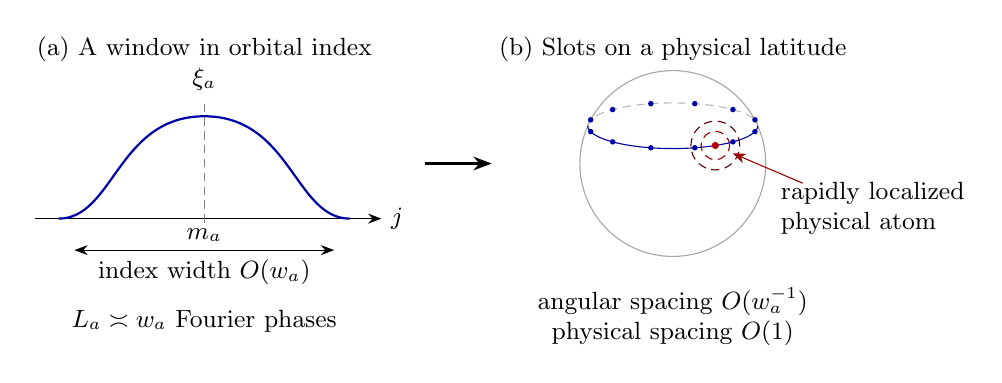
\begin{tikzpicture}[x=1cm,y=1cm,>=Stealth,font=\small]
 \begin{scope}
  \node[anchor=west] at (-.1,2.5) {(a) A window in orbital index};
  \draw[->] (0,.35)--(4.4,.35) node[right] {$j$};
  \draw[blue!65!black,thick]
     (.3,.35)..controls (1,.35) and (1.05,1.65)..(2.15,1.65)
     ..controls (3.25,1.65) and (3.3,.35)..(4,.35);
  \draw[densely dashed,gray] (2.15,.3)--(2.15,1.85);
  \node[above] at (2.15,1.85) {$\xi_a$};
  \draw[<->] (.5,-.05)--(3.8,-.05)
       node[midway,below] {index width $O(w_a)$};
  \node[below] at (2.15,.35) {$m_a$};
  \node[align=center] at (2.15,-.95)
       {$L_a\asymp w_a$ Fourier phases};
 \end{scope}
 \draw[->,thick] (4.95,1.05)--(5.8,1.05);
 \begin{scope}[shift={(8.1,1.05)}]
  \node at (0,1.45) {(b) Slots on a physical latitude};
  \draw[gray!70] (0,0) circle (1.18);
  \draw[gray!55,densely dashed] (-1.08,.48)
      arc[start angle=180,end angle=0,x radius=1.08,y radius=.29];
  \draw[blue!65!black] (-1.08,.48)
      arc[start angle=180,end angle=360,x radius=1.08,y radius=.29];
  \foreach \a in {15,45,...,345}
    {\fill[blue!65!black] ({1.08*cos(\a)},{.48+.29*sin(\a)}) circle (.035);}
  \fill[red!70!black] (.54,.229) circle (.045);
  \draw[red!60!black,densely dashed] (.54,.229) circle (.18);
  \draw[red!35!black,densely dashed] (.54,.229) circle (.31);
  \draw[->,red!60!black] (1.65,-.25)--(.76,.13);
  \node[align=left,anchor=west] at (1.25,-.57)
       {rapidly localized\\physical atom};
  \node[align=center] at (0,-1.95)
       {angular spacing $O(w_a^{-1})$\\physical spacing $O(1)$};
 \end{scope}
\end{tikzpicture}
\caption{The index window has width comparable to $w_a$; its Fourier
phases place a comparable number of slots around the latitude.
Together with unit-order radial spacing, this gives bounded slot
density in physical distance.  The drawing is schematic: dashed
circles indicate rapidly decaying tails, not compact spatial support.}
\label{fig:local-slots}
\end{figure}

We need two quantitative consequences of this construction.  Let $k_y$
be a normalized coherent orbital centered at $y$.

\begin{lemma}[Uniform frame localization]\label{locality:frame}
For every $D$ there is $C_D$ such that
\begin{equation}
 |\langle z_x,k_y\rangle|\leq C_D(1+d(x,y))^{-D}.
 \label{eq:frame-coherent-decay}
\end{equation}
For two frames constructed as above, possibly with different axes, their
atoms satisfy the same bound with $k_y$ replaced by an atom centered at
$y$.  For each fixed integer $J$, \eqref{eq:frame-coherent-decay} also
holds, with constants depending on $J$, for every rotated polar orbital
$e_j(y)$ with $0\leq j\leq J$.
\end{lemma}

\begin{proof}
Choose the axial gauge and azimuth convention in which the coefficient
of $e_j$ in $k_y$ is $e^{ij\phi_y}p_{q,m}(j)^{1/2}$.  Its modulus is
\[
 p_{q,m}(j)^{1/2},\qquad
 p_{q,m}(j)=\binom qj(m/q)^j(1-m/q)^{q-j}.
\]
They obey, after extension by zero outside $[0,q]$,
\begin{equation}
 |\Delta^l p_{q,m}(j)^{1/2}|
 \leq C_{D,l}w_q(m)^{-1/2-l}
       \left(1+\frac{|j-m|}{w_q(m)}\right)^{-D}.
 \label{eq:binomial-symbol}
\end{equation}
Here and below finite differences may shift the argument by a fixed
number of indices, which only changes the constant.  We include a
verification to specify uniformity near the ends.  First put $p=m/q$
and $\sigma^2=qp(1-p)$, so
$w_q(m)^2=1+q\sigma^2/(q+1)\asymp1+\sigma^2$.
Fourier inversion of a binomial law of variance $\sigma^2$ gives
\[
 \sup_j p_{q,m}(j)\leq\frac1{2\pi}\int_{-\pi}^{\pi}
       \bigl(1-4p(1-p)\sin^2(t/2)\bigr)^{q/2}\,dt
       \leq \frac C{1+\sigma}.
\]
For $0<p<1$, tilt the law by $e^{\lambda j}$.  Its new parameter is
$p_\lambda=pe^\lambda/(1-p+pe^\lambda)$, and its variance differs
from $\sigma^2$ by a factor between $e^{-|\lambda|}$ and
$e^{|\lambda|}$.  Therefore the centered log moment generating
function satisfies
$\log\mathbb E e^{\lambda(X-m)}\leq\sigma^2\lambda^2$
for $|\lambda|\leq1/2$.  At $z=j-m$, choose
$\lambda=z/(2(\sigma^2+|z|))$.  The exact tilting identity and the
preceding point-mass bound give
\begin{equation}
 p_{q,m}(j)\leq\frac C{w_q(m)}
       \exp\left(-\frac{c|j-m|^2}{w_q(m)^2+|j-m|}\right).
 \label{eq:binomial-global-tail}
\end{equation}
The cases $p=0,1$ are direct.  This proves every polynomial tail
bound with the required height, uniformly also when $w_q(m)$ is
bounded.

For the derivative gain first assume $w_q(m)^2\geq16(l+1)$, and let
$h=\min(m,q-m)\asymp w_q(m)^2$.  Interpolate the square root of the
binomial probability by gamma functions, writing the resulting
positive function as $F(x)$.  Put $\psi=(\log\Gamma)'$ and
$\psi_1=(\log\Gamma)''$.  On $|x-m|\leq h/2$, the explicit
formulas
\[
 \begin{aligned}
 (\log F)'(x)=\tfrac12\left(\log\frac p{1-p}
          -\psi(x+1)+\psi(q-x+1)\right),\\
 (\log F)''(x)=-\tfrac12\bigl(\psi_1(x+1)+\psi_1(q-x+1)\bigr)
 \end{aligned}
\]
and the positive-real polygamma series give
$|(\log F)'(m)|\leq Cw^{-2}$,
$(\log F)''(x)\leq-cw^{-2}$, and
$|(\log F)^{(k)}(x)|\leq C_kw^{-k}$ for $k\geq2$.
Stirling's inequalities give $F(m)\leq Cw^{-1/2}$.
Differentiating $F=e^{\log F}$ consequently proves
\[
 |F^{(l)}(x)|\leq C_{D,l}w^{-1/2-l}
                    (1+|x-m|/w)^{-D},\qquad |x-m|\leq h/2.
\]
If $|j-m|\leq h/4$, integrate this derivative over the unit cube
that represents $\Delta^lF(j)$; the entire stencil stays in the
displayed interval.  Outside that region, each nonzero stencil
entry has $|j+a-m|\geq cw^2$, $0\leq a\leq l$.
Equation~\eqref{eq:binomial-global-tail} then supplies an
exponential in that distance, which pays both $w^{-l}$ and every
polynomial tail.  This also handles stencils crossing an endpoint.
Finally, if $w^2<16(l+1)$, bound the finite difference by its $l+1$
values and use \eqref{eq:binomial-global-tail}; the factor $w^{-l}$
is now a constant depending only on $l$.  This completes the proof
of \eqref{eq:binomial-symbol}, including the bounded-width regime.

Insert \eqref{eq:binomial-symbol} in \eqref{eq:frame-atoms}.  For windows
whose radial centers are a bounded distance apart, their widths are
comparable; summation by parts $l$ times gives the factor
$(1+w_a|\phi_x-\phi_y|)^{-l}$, with angular difference modulo $2\pi$.
The absolute sum before summation by parts is bounded.  For separated
radial windows, the tail in \eqref{eq:binomial-symbol} first supplies
arbitrary powers of radial distance.  The ratios of the widths cost
only polynomial powers by \eqref{eq:local-scale-ratios}.  Spending
additional tail orders therefore gives the same angular estimate.
Radial distance plus the shorter latitude arc bounds the spherical
distance from above, proving \eqref{eq:frame-coherent-decay}.

The coherent resolution of the identity has density
$(q+1)/(2\pi q)$ with respect to area.  Inserting it between two frame
atoms reduces the frame-to-frame bound to
\[
 \int_{S_q}(1+d(x,z))^{-D-3}(1+d(z,y))^{-D-3}\,dz
 \leq C_D(1+d(x,y))^{-D}.
\]
The inequality follows by dividing the integral into the sets where
$d(x,z)\geq d(x,y)/2$ and where $d(z,y)\geq d(x,y)/2$.
Finally
\[
 |\langle e_j(y),k_z\rangle|^2
 =\binom qj\sin^{2j}(\vartheta/2)\cos^{2(q-j)}(\vartheta/2),
\]
where $\vartheta$ is the angle between $y$ and $z$.  For bounded $j$,
this is bounded by $C_j(1+d(y,z))^{2j}e^{-c d(y,z)^2}$; increasing the
constant covers bounded $q$.  Inserting the coherent resolution once
more proves the last assertion.
\end{proof}

\begin{lemma}[Common frames for nearby fluxes]\label{locality:common-frames}
For each fixed $d_0$, frames at fluxes $q$ and $t$ with
$0\leq q-t\leq d_0$ may be embedded in the same slots so that index
identification $i_{q,t}:e_j^{(t)}\mapsto e_j^{(q)}$, $j\leq t$,
satisfies the exact identity $\mathsf S_t=\mathsf S_q i_{q,t}$.
All preceding estimates remain uniform.  In the northern third the
windows can be chosen from one system independent of the flux; there
one may use the common metric with radial variable $\sqrt{1+m}$.
\end{lemma}

\begin{proof}
Use the windows and Fourier lengths at flux $q$ for both spaces, and
restrict their index sequences to $0\leq j\leq t$ for the smaller
space.  Equation~\eqref{eq:tight-frame} still holds on those indices.
Only a bounded number of end indices have been removed.  The windows
meeting them have bounded width, or have rapidly small tails in the
estimates in which an endpoint extension occurs.  The slot positions
for the two sphere metrics differ by a bounded distance; the constants
may depend on $d_0$.  For all sufficiently large $q$, every window
centered in the northern third has its full support below $q/2$,
because its width is $O(\sqrt q)$.  On these supports the construction
uses only $\eta(\sqrt{1+j}-k)$ and their fixed normalization, and
their Fourier length is the fixed integer $16(k+1)$.  These complete
slot vectors are therefore independent of $q$ in index coordinates.
The buffer between $q/3$ and $q/2$ permits changing the frame outside
this region without changing its northern slots.  Bounded fluxes may
use pairwise padded frames; no long sequence of common slots is needed
there.
\end{proof}

Whenever operators at these two fluxes are subtracted, we first use
$i_{q,t}$ and extend the smaller operator by the identity on the
added orbital modes.  Thus, under the graded decomposition
$\mathcal F_q=\mathcal F_t\,\widehat\otimes\,
\bigwedge\operatorname{span}\{e_{t+1},\ldots,e_q\}$, the padded
operator is $A\widehat\otimes I$.  Extra modes are put in their
vacuum only when comparing states or taking the physical compression.

The fermionic Fock space over $\ell^2(\Lambda_q)$ is a graded tensor
product of two-dimensional slot spaces.  The exterior isometry
$\Gamma(\mathsf S_q)$ identifies $\mathcal F_q$ with the subspace in which
the orthogonal complement of $\mathsf S_qU_q$ is vacant.  A \emph{physical}
operator is an operator in the CAR algebra generated by $\mathsf S_qU_q$,
extended as the identity on the complementary modes.  It preserves
that vacant-complement subspace.  For $X\subset\Lambda_q$, let
$\mathfrak A(X)$ be the CAR algebra of its slots.  Put
$\mathcal N_{\mathrm{slot}}=\sum_{x\in\Lambda_q}c_x^*c_x$.
An operator has number grade $k\in\mathbb Z$ if
$[\mathcal N_{\mathrm{slot}},A]=kA$, and parity
$\epsilon_A\in\{0,1\}$ if
$(-1)^{\mathcal N_{\mathrm{slot}}}A(-1)^{\mathcal N_{\mathrm{slot}}}
=(-1)^{\epsilon_A}A$.  Operators of even parity on disjoint sets
commute; homogeneous operators obey the
graded relation
\[
 [A,B]_{\mathrm{gr}}=AB-(-1)^{\epsilon_A\epsilon_B}BA=0.
\]
All Hamiltonians below have even parity.  Local expansions can be
projected onto any prescribed number grade by averaging the gauge
action of the total slot number $\mathcal N_{\mathrm{slot}}$.
This action preserves every slot algebra and does not increase
approximation errors.  On physical operators its grading agrees with
that of the physical number operator $\mathcal N$.

\subsection{Local norms and summation}

For a center $x$, an operator $A$, and $l>0$, define
\begin{equation}
 \|A\|_{x,l}=\|A\|+
 \sup_{r\geq1}(1+r)^l
       \inf_{A_r\in\mathfrak A(B_r(x))}\|A-A_r\|.
 \label{locality:ball-norm}
\end{equation}
We call $A$ rapidly local at $x$ if this is finite for every $l$,
with bounds uniform in the volume under consideration.  An interaction
is a family $A_x$ integrated against a measure whose mass in every
unit ball is bounded.  A bound of \emph{size} $a(x)$ means
$\|A_x\|_{x,l}\leq C_l a(x)$ for every $l$.  A positive function $a$
is called tempered if, for fixed $C,\kappa$,
\begin{equation}
 a(x)\leq C a(y)(1+d(x,y))^\kappa.
 \label{eq:tempered-weight}
\end{equation}
The constants in estimates involving $a$ may depend on $C,\kappa$.
Powers and products of $u,v,w$ are examples.

Taking near-best approximations at radii $2^k$ and subtracting successive
ones gives a ball decomposition
\begin{equation}
 A=\sum_{k\geq0}A^{(k)},\qquad
 A^{(k)}\in\mathfrak A(B_{2^{k+1}}(x)),\qquad
 \|A^{(k)}\|\leq C_l\|A\|_{x,l}2^{-kl}.
 \label{eq:ball-decomposition}
\end{equation}
Conversely such a decomposition implies the approximation bound, with
any slightly smaller exponent.  We use this elementary equivalence
to pass between operators and interactions on balls.

An observable supported initially on a large ball needs a separate
convention.  A family has \emph{core radius $r$ and amplitude $a$} if
\begin{equation}
 \|A\|\leq Ca,\qquad
 \inf_{A_R\in\mathfrak A(B_R(x))}\|A-A_R\|
       \leq C_Da(1+R)^{-D}\quad(R\geq C_*r),
 \label{eq:local-core-tail}
\end{equation}
where the geometric constant $C_*$ is independent of $D$.
The amplitude may contain a specified power of $r$.  This convention
does not assert that every centered norm \eqref{locality:ball-norm}
is bounded by $Ca$ without a further radius factor.

\begin{lemma}[Shells outside a fixed core]\label{locality:core-shells}
If \eqref{eq:local-core-tail} holds with $r\geq1$, there is a
decomposition $A=\sum_{\nu\geq0}A_\nu$ with
$A_\nu\in\mathfrak A(B_{C_*2^{\nu+1}r}(x))$ and
$\|A_\nu\|\leq C_Da2^{-\nu D}$ for every $D$.
Consequently, for each fixed $B\geq0$,
\begin{equation}
 \sum_{\nu\geq0}(C_*2^{\nu+1}r)^B\|A_\nu\|
       \leq C_Ba r^B.
 \label{eq:local-core-moment}
\end{equation}
\end{lemma}

\begin{proof}
Take approximants at radii $C_*2^\nu r$ and telescope, starting
with the first approximant as the core.  The core norm is $Ca$;
the other differences are bounded by the two adjoining errors in
\eqref{eq:local-core-tail}.  Sum with any $D>B+1$ to obtain
\eqref{eq:local-core-moment}.
\end{proof}

\begin{lemma}[Products, commutators, and weighted sums]
\label{locality:calculus}
The following bounds are uniform over the slot systems above.
\begin{enumerate}
\renewcommand{\labelenumi}{\textup{(\roman{enumi})}}
\item Products of operators rapidly local at the same center, and
adjoints, preserve rapid locality.  If $A,B$ are
centered at $x,y$, respectively, with bounded local norms, then
$\|[A,B]_{\mathrm{gr}}\|\leq C_D(1+d(x,y))^{-D}$ for every $D$.
\item If $A$ is rapidly local at $x$ and a rapidly local interaction
$K_y$ has tempered size $a(y)$, then
$[\int K_y\,dy,A]_{\mathrm{gr}}$ is rapidly local at $x$, of size
$a(x)$ times the local bounds of $A$.
\item Suppose $A$ is even, $\|A\|_{x,l}\leq1$, and $J_y$ has bounded
rapid local norms.  With $D=1+d(x,y)$ and $C_{xy}=[A,J_y]$,
\begin{equation}
 \|C_{xy}\|\leq C D^{-l},\qquad
 \|C_{xy}\|_{x,l}\leq C,\qquad
 \|C_{xy}^*C_{xy}\|_{x,l}\leq C D^{-l}.
 \label{eq:commutator-square-locality}
\end{equation}
\end{enumerate}
For an operator initially supported in $B_r(x)$, the corresponding
core estimates cost a fixed polynomial in $r$.  At distances larger
than a fixed multiple of $r$, any prescribed decay order is available.
\end{lemma}

\begin{proof}
The product estimate follows from
\[
 \|AB-A_rB_r\|
 \leq\|A-A_r\|\|B\|+\|A_r\|\|B-B_r\|.
\]
For the commutator use approximations of radius less than $d(x,y)/3$;
their graded commutator vanishes.  For the weighted assertion expand
both factors as in \eqref{eq:ball-decomposition}.  Terms with disjoint
balls vanish, while intersecting balls of radii $R,S$ require
$d(x,y)\leq R+S$.  The number or measure of their possible centers is
$O((1+R+S)^2)$, and \eqref{eq:tempered-weight} costs at most
$C(1+R+S)^\kappa$.  To obtain an output moment of order $D$, bound
these costs by $C(1+R+S)^{D+\kappa+2}$ and choose input decay order
larger than $D+\kappa+6$.  The two geometric sums then converge.
This argument also permits assigning each output term to the center
of either input; that convention will be used for differences of
interactions.

For \eqref{eq:commutator-square-locality}, the first estimate follows
by the disjoint-ball argument at exponent $l$.  For approximation
radii $r\leq3D$, use zero as an approximant to $C_{xy}$, giving
$r^l\|C_{xy}\|\leq C$.  For $r>3D$, approximate $A$ in $B_{r/3}(x)$
and $J_y$ in $B_{r/3}(y)$; their commutator is supported in $B_r(x)$
and has error $Cr^{-l}$.  Thus the second estimate holds.  Apply the
product estimate with the small norm $\|C_{xy}\|\leq CD^{-l}$ on one
factor to obtain the third estimate.  Finally a ball $B_r(x)$ contains
$O((1+r)^2)$ slots, and tempered ratios within it cost
$O((1+r)^\kappa)$.  The same sums give the stated polynomial core
costs.  For tails beyond $Cr$, the distance from the original ball
is comparable to the tail radius, so increasing a tail order does not
increase the core-volume exponent.
\end{proof}

\begin{corollary}[The physical interactions]\label{locality:basic-interactions}
\label{locality:toeplitz}
The unperturbed Hamiltonian $H_q$ and the Fock lift of any bounded
real scalar symbol $\varphi$ have physical, neutral, Hermitian rapid
interactions of uniform sizes $C_D$ and $C_D\|\varphi\|_\infty$,
respectively.
\end{corollary}

\begin{proof}
Coefficient localization gives operator-norm localization directly.
If $E_R$ is the one-particle projection onto slots in $B_R(x)$, the
CAR identity $\|c(f)\|=\|f\|_2$ gives
\[
 \|c(\mathsf S_q f)-c(E_R\mathsf S_q f)\|
       =\|(I-E_R)\mathsf S_q f\|_2.
\]
For $f=k_x$ or a bounded polar mode at $x$,
Lemma~\ref{locality:frame} and the slot count
\eqref{eq:slot-volume} make the right side at most
$C_D(1+R)^{-D}$ for every $D$; the approximating annihilator is
supported in $B_R(x)$.

The coherent resolution gives
\[
 d\Gamma(T_q(\varphi))=\frac{q+1}{2\pi q}
       \int_{S_q}\varphi(x)c^*(k_x)c(k_x)\,dA(x).
\]
For $H_q$, the highest pair vector is $v_0=e_0\wedge e_1$.
Schur's Lemma on the spin-$(q-1)$ pair space and its dimension
$2q-1$ give, with Haar mass one,
\begin{equation}
 H_q=(2q-1)\int_{SU(2)}B(gv_0)^*B(gv_0)\,dg.
 \label{eq:coherent-pair-resolution}
\end{equation}
The product $B(gv_0)=c(ge_1)c(ge_0)$ is rapidly local at the
rotated pole by Lemmas~\ref{locality:frame} and
\ref{locality:calculus}.  Its phase along the stabilizer disappears
in its square, so the center measure on the sphere has density
$(2q-1)/(2\pi q)$.  This and $(q+1)/(2\pi q)$ are uniformly bounded.
The same two lemmas localize $c^*(k_x)c(k_x)$.  No derivative of
$\varphi$ enters either the representation or its bound.
\end{proof}

\subsection{Propagation and spectral filters}

We next establish that a time filter preserves this local calculus.
The relevant propagation bound is needed only with arbitrary polynomial
decay, which permits a direct truncation argument.  The underlying
commutator iteration is the Lieb--Robinson method
\cite{LR}, in its graded fermionic form \cite{NSY}; its use with time filters is the locality
mechanism behind quasi-adiabatic continuation and spectral flow
\cite{HW,BMNS}.

\begin{lemma}[Propagation of local observables]\label{locality:dynamics}
Let $K$ be self-adjoint and even, with a rapidly local interaction of
uniform size.  Write $\tau_t^K(A)=e^{itK}Ae^{-itK}$.  For each $D$
there are $D'$ and $M_D$, independent of volume, such that
\begin{equation}
 \|\tau_t^K(A)\|_{x,D}
       \leq C_D(1+|t|)^{M_D}\|A\|_{x,D'}.
 \label{eq:polynomial-propagation}
\end{equation}
The assertion holds also for time-dependent generators with the same
uniform bounds.  In particular evolution over a bounded parameter
interval preserves rapid locality.  If $A$ is supported in $B_r(x)$,
the error in approximating $\tau_t^K(A)$ on $B_R(x)$, for
$R\geq C(r+(1+|t|)^4)$, is bounded by
$C_D\|A\|(1+r)^2R^{-D}$.
\end{lemma}

\begin{proof}
Use \eqref{eq:ball-decomposition} to write $K$ as a sum of terms on
balls.  Taking Hermitian and even parts makes each term Hermitian
and even without changing the total or its estimates.  First retain
only terms of diameter at most $\ell$.  For
this truncated interaction define
\[
 M_{ab}=2\sum_{X\ni a,b}\|K_X\|.
\]
Uniform summability, including the number of sites in $X$, gives
$\sup_a\sum_b M_{ab}e^{d(a,b)/\ell}\leq C$; indeed each retained
distance is at most $\ell$, and the ball-volume costs are polynomial.
The iterated commutator inequality, with internal evolution removed
unitarily at each step, therefore gives
\begin{equation}
 \|[\tau_t^{K_{\leq\ell}}(A),B]_{\mathrm{gr}}\|
 \leq C\|A\|\|B\|\,|X|\,|Y|
        e^{C|t|-d(X,Y)/\ell}
 \label{eq:truncated-LR}
\end{equation}
for $A\in\mathfrak A(X)$ and $B\in\mathfrak A(Y)$.
For completeness, the $n$th iterated integral contributes $|t|^n/n!$
times a chain of $n$ matrix factors $M$.  Multiplication by
$e^{d(X,Y)/\ell}$ is bounded by the product of the exponential
weights along the chain.  Summing the intermediate sites gives
$C^n$, and summing $n$ gives \eqref{eq:truncated-LR}.  Evenness of
the generator makes the same calculation valid for odd $A,B$ with
the graded commutator.

Restore the removed terms using Duhamel's formula.  For each removed
ball term use the smaller of the trivial commutator bound and
\eqref{eq:truncated-LR}.  The centers within distance
$C\ell(1+|t|)$ of $X$, together with the radius of that term, occupy
at most a polynomial volume.  Outside that region the exponential
bound is summable.  Consequently, for every $s$, the restoration
error is at most
\begin{equation}
 C_s\|A\||X|(1+|t|)
       (1+r+\ell(1+|t|))^4\ell^{-s},
 \label{eq:range-restoration}
\end{equation}
when $X\subset B_r(x)$.  To see the power allowance explicitly, a
removed term of radius $a$ contributes its norm times at most
$C(1+r+\ell(1+|t|)+a)^2$ possible centers and at most
$C(1+a)^2$ sites.  Its arbitrarily high radius moment makes the sum
over $a>\ell/2$ bounded by the right side of
\eqref{eq:range-restoration}, after increasing the input moment by
$s+6$.

Now let $R\geq C(r+(1+|t|)^4)$ and choose $\ell=R^{1/3}$.
The truncated evolution differs from the evolution generated by its
terms contained in $B_R(x)$ by
$C\|A\||X|\operatorname{poly}(R)e^{C|t|-cR^{2/3}}$.
This is again Duhamel's formula and \eqref{eq:truncated-LR}, summed
over the boundary terms.  Both restoration errors are bounded by
$C_D\|A\||X|R^{-D}$, choosing $s$ sufficiently large in
\eqref{eq:range-restoration}.  This supplies an approximation in
$\mathfrak A(B_R(x))$.  At smaller radii use the norm bound
$\|\tau_t(A)\|=\|A\|$.  Since $|X|\leq C(1+r)^2$, this proves the
assertion for supported $A$ and then, by
\eqref{eq:ball-decomposition}, \eqref{eq:polynomial-propagation}.
The proof uses only uniform bounds on the interaction at each time,
so also proves the time-dependent assertion.
\end{proof}

\begin{lemma}[Time filters]\label{locality:filters}
Suppose $F\in L^1(\mathbb R)$ and
$\int(1+|t|)^j|F(t)|\,dt<\infty$ for every $j$.  Under the hypotheses
of Lemma~\ref{locality:dynamics},
\begin{equation}
 \mathcal T_{F,K}(A)=\int_{\mathbb R}F(t)\tau_t^K(A)\,dt
 \label{eq:time-filter}
\end{equation}
is rapidly local whenever $A$ is, with uniform bounds.  The same is
true for a finite measure consisting of such a function and a mass at
zero.  Number grade and physicality are preserved when $K$ is neutral
and physical.  Suitable symmetry of $F$ preserves adjoints.
\end{lemma}

\begin{proof}
Integrate \eqref{eq:polynomial-propagation}.  The approximation norm
is a seminorm up to its operator-norm summand, so the integral of local
approximants gives the required estimate.  The remaining assertions
follow directly by commuting the evolution with gauge transformations,
the physical algebra, and adjoints.
\end{proof}

The frequency functions used below are smooth, vanish on an interval
about zero, and have tails proportional to $1/\omega$ on one or both
half-lines.  Their inverse Fourier transforms satisfy the hypotheses
of Lemma~\ref{locality:filters}.  Here is a convenient verification.
Every positive-order derivative of such a multiplier is integrable,
so integration by parts gives arbitrary powers of decay for $|t|\geq1$.
For $0<|t|<1$, split the frequency integral at $|\omega|=|t|^{-1}$.
The inner portion is $O(1+|\log|t||)$, and one integration by parts
on the outer portion is $O(1)$.  Thus the possible singularity at
zero is integrable.  A smooth compactly supported multiplier has a
Schwartz kernel.  These facts cover both spectral transport and
the filters that retain only small energy differences.

\begin{lemma}[Weighted differences]\label{locality:difference}
Let $K,K'$ satisfy Lemma~\ref{locality:dynamics} uniformly, and assume
$K-K'$ has a rapidly local interaction of tempered size $a(z)$.
For a rapidly local $A$ centered at $x$,
\begin{equation}
 \|\tau_t^K(A)-\tau_t^{K'}(A)\|_{x,D}
 \leq C_Da(x)(1+|t|)^{M_D}\|A\|_{x,D'}.
 \label{eq:weighted-evolution-difference}
\end{equation}
The same conclusion holds after an all-moments time filter, and for
differences of bounded-parameter evolutions.  If the input itself
changes by local size $b(x)$, its separate contribution is $Cb(x)$.
All estimates retain the product of a local input size and $a(x)$.
If $A\in\mathfrak A(B_r(x))$, put $s=\kappa+2$, with $\kappa$ from
\eqref{eq:tempered-weight}.  The difference has operator norm at most
\begin{equation}
 C a(x)\|A\|(1+r)^s|t|(1+|t|)^{4s}.
 \label{eq:difference-core}
\end{equation}
For $R\geq C_*(1+r)$, with a fixed geometric constant $C_*$, it has
an approximation supported in $B_{r+R}(x)$
with error at most
\begin{equation}
 C_Da(x)\|A\|(1+r)^s
        (1+|t|)^{4D+4s+1}(1+R)^{-D}.
 \label{eq:difference-tail}
\end{equation}
Thus the power of the initial radius is independent of the tail order.
If the differing interaction vanishes throughout a ball of radius $d$
about $x$, the bounds for a fixed rapidly local input gain arbitrary
inverse powers of $1+d$.
\end{lemma}

\begin{proof}
Use the exact formula
\[
 \tau_t^K(A)-\tau_t^{K'}(A)
 =i\int_0^t\tau_s^K
       ([K-K',\tau_{t-s}^{K'}(A)])\,ds.
\]
Apply Lemma~\ref{locality:dynamics} to the inside observable,
Lemma~\ref{locality:calculus}(ii) to the commutator, and
Lemma~\ref{locality:dynamics} once more to the outside evolution.
The tempered inequality \eqref{eq:tempered-weight} is precisely what
allows the insertion at $z$ to be charged to $a(x)$.  All time costs
are polynomial and therefore integrable against the specified
filters.  The time-dependent version follows from its identical
Duhamel formula.  Linearity handles a changed input.

We give the additional radius bookkeeping for
\eqref{eq:difference-core}--\eqref{eq:difference-tail}.
For a ball decomposition about $x$, use the weighted sum
$\sum_R(1+R)^p\|A_R\|$.  Lemma~\ref{locality:dynamics} bounds its
evolved value by $C_p(1+|t|)^{4p}$ times its initial value.  Indeed,
for a radius-$r$ input, begin a dyadic decomposition at
$Q=C(1+r+(1+|t|)^4)$.  The core contributes $C\|A\|Q^p$;
the subsequent shells contribute at most
$C_M\|A\|(1+r)^2\sum_{R\geq Q}R^{p-M}$.
Choosing $M>p+2$ bounds this by $C_p\|A\|Q^p$.
The weighted insertion estimate in the proof of
Lemma~\ref{locality:calculus} costs $s=\kappa+2$ powers of the input
radius.  Duhamel at $p=0$ proves \eqref{eq:difference-core}.

For the tail first take $|t|\leq cR^{1/4}$ in the Duhamel integrand,
with $c>0$ a sufficiently small fixed constant; bounded $R$ are
covered by \eqref{eq:difference-core}.  Fix also a small $\varepsilon>0$.
Choose $\varepsilon,c$ and then $C_*$ so that the propagation lemma
applies both from radius $r$ to $r+\varepsilon R$ and from radius
$r+3\varepsilon R$ to $r+R$.  This requires only fixed constants:
if $C$ is the constant in that lemma, take
$\varepsilon<(100C)^{-1}$, $c^4<\varepsilon/(10C)$, and
$C_*>100C/\varepsilon$.
Cut the inner evolved observable at radius $r+\varepsilon R$.  Its remaining
shells have weighted sum of order $s$ at most
$C_M\|A\|(1+r)^2R^{s-M}$, by the short-time bound in
Lemma~\ref{locality:dynamics}; their commutator with the insertion
has the same bound times $Ca(x)$.  In the retained part, discard
insertion terms of radius greater than $\varepsilon R$.  Their arbitrary
radius moments give an error $C_Ma(x)\|A\|R^{-M}$.
The remaining commutator is supported in $B_{r+3\varepsilon R}(x)$ and has
norm at most $Ca(x)\|A\|R^s$.  Evolving it in the outside factor
of Duhamel and using the short-time propagation estimate gives
an approximation on $B_{r+R}(x)$ with error
$C_Ma(x)\|A\|R^{s+2-M}$.
Choose $M$ in each of these three bounds larger than the requested
order plus $s+4$, and integrate over an interval of length at most
$R^{1/4}$.  This gives the stated tail bound for short times.
For $|t|>cR^{1/4}$, use \eqref{eq:difference-core} and
$(1+|t|)^{4D}(1+R)^{-D}\geq c_D$.

Finally suppose an insertion ball of radius $a$ can occur only if
its center $z$ satisfies $d(x,z)+a\geq d$.  If that ball meets an
input shell of radius $R$, then $d\leq R+2a$.  Inserting
$(1+d)^{-M}(1+R+2a)^M$ into the shell summation proves the last
assertion, after increasing the input moments.  This includes changes
supported outside a common comparison region.
\end{proof}

To specify physical compression, let $S:U_q\to K_S$ and
$T:U_q\to K_T$ be two slot analysis isometries.  Write $J_S=\Gamma(S)$
for the vacuum-complement embedding and $\iota_T$ for the embedding of
the physical CAR algebra into the output slots, acting as the identity
on complementary modes.  The map that we estimate is
\begin{equation}
 \mathcal C_{T\leftarrow S}(A)
   =\iota_T(J_S^*AJ_S).
 \label{eq:physical-compression-map}
\end{equation}
When $T=S$ this is compression followed by identity extension; it is
a unital contractive completely positive map.  On physical input
operators it is simply change of frame.

\begin{lemma}[Compression, changes of frame, and smooth functions]
\label{locality:functional-calculus}
The map \eqref{eq:physical-compression-map}, for the frames of
Lemma~\ref{locality:frame}, preserves rapid locality.  An
operator supported in $B_r(x)$ remains localized about that ball,
with polynomial core costs and arbitrary inverse-power tails outside
$B_{Cr}(x)$.  If $A=A^*$ is bounded and rapidly local, and $f$ is
smooth on a neighborhood of its spectrum, then $f(A)$ is rapidly
local.  The constants depend on finitely many local bounds and
derivatives for each requested decay order.
\end{lemma}

\begin{proof}
Put two slot spaces side by side.  If $S,T$ are their analysis
isometries, the partial isometry $TS^*$ has rapidly decaying matrix
entries by Lemma~\ref{locality:frame}.  On their direct sum, the
anti-self-adjoint one-particle operator
\[
 \begin{pmatrix}0&-ST^*\\TS^*&0\end{pmatrix}
\]
rotates the two physical subspaces into each other through angle
$\pi/2$ and acts as zero on their complements.  Its second
quantization is a bounded-strength, rapidly local quadratic
interaction: absolute row sums and every distance moment are bounded
by \eqref{eq:slot-volume}.  Lemma~\ref{locality:dynamics} applies
over this fixed angle.  Conjugate $A\otimes I$ by this rotation and
take the vacuum expectation in the entire first slot copy, retaining
the entire second copy.  On a CAR monomial, the physical components
have moved from $S U_q$ to $T U_q$, while the complementary components
in the first copy are evaluated in their vacuum.  The resulting map
is exactly \eqref{eq:physical-compression-map}, including for odd
monomials; linearity gives the identity for every operator.  Vacuum
expectation is contractive and preserves support in the doubled slot
geometry.  This proves the assertion, and $S=T$ gives re-embedded
physical compression.  In particular no projection onto the output
complementary vacuum is left in the resulting operator.

For the functional-calculus assertion extend $f$ smoothly to a compactly
supported function on $\mathbb R$.  If $A_r$ approximates $A$ locally,
its Hermitian part does so with the same error.  The Fourier formula
and Duhamel's identity give
\[
 \|f(A)-f(A_r)\|
 \leq\left(\int_{\mathbb R}|t|\,|\widehat f(t)|\,dt\right)
       \|A-A_r\|.
\]
Since $f(A_r)$ belongs to the same local algebra, the approximation
bounds follow.  A constant value of $f$ contributes only a scalar
identity, which is local in every ball.
\end{proof}

\subsection{Pair rows and diagonal symbols}

The coherent orbit representations already prove locality of the
unperturbed Hamiltonian and bounded scalar perturbations.  Pinning zeros
will deform the pair coefficients and remove full rotation invariance.
To control those deformations and compare neighboring fluxes, we now
prove a local calculus directly for angular-momentum rows and diagonal
orbital symbols.

Write $Q_b=B_{b-1}$ for the normalized pair annihilator with index
sum $b$ in \eqref{eq:pair-rows}, $1\leq b\leq2q-1$.  Define its
ordered coefficients by
\begin{equation}
 a_b(i)=\frac{(b-2i)\sqrt{\binom qi\binom q{b-i}}}{\sqrt{S_b}},
 \qquad
 S_b=\binom{2q}{b}\frac{b(2q-b)}{2q-1}.
 \label{eq:pair-symbol-normalization}
\end{equation}
In this formula the sum for $S_b$ is over ordered $i$.  With a fixed
choice of annihilator sign,
$Q_b=2^{-1/2}\sum_{i+j=b}a_b(i)c_jc_i
=\sqrt2\sum_{i<j,\,i+j=b}a_b(i)c_jc_i$.
Changing this common sign leaves every square unchanged.

\begin{lemma}[Pair profiles and local row squares]
\label{locality:row-symbols}
With $m=b/2$ and $w=w_q(m)$, the zero-extended coefficients satisfy
\begin{equation}
 |\Delta_i^r\Delta_b^s a_b(i)|
 \leq C_{D,r,s}w^{-1/2-r-s}
       \left(1+\frac{|i-m|}{w}\right)^{-D}.
 \label{eq:pair-row-symbols}
\end{equation}
There are pair annihilators $L_{\nu,\phi}$, rapidly local with uniform
bounds about centers $x_{\nu,\phi}$, and a measure $d\mu$ of bounded
mass per unit ball, such that
\begin{equation}
 H_q=\sum_\nu\int_0^{2\pi}
                L_{\nu,\phi}^*L_{\nu,\phi}\,d\mu_\nu(\phi).
 \label{eq:pair-local-resolution}
\end{equation}
The construction is linear in the row coefficients.  In particular
symbol bounds \eqref{eq:pair-row-symbols} with an additional tempered
factor give local bounds with that factor; the same holds for
differences of row families in common frames.
\end{lemma}

\begin{proof}
Vandermonde's identity identifies
$\binom qi\binom q{b-i}/\binom{2q}{b}$ as a hypergeometric law of
mean $b/2$ and variance $b(2q-b)/(4(2q-1))$.
Multiplying its second centered moment by four proves
\eqref{eq:pair-symbol-normalization}.  The moment formula itself
also follows directly by applying
$i\binom qi=q\binom{q-1}{i-1}$ twice and Vandermonde's identity.

Here are symbol estimates that include the dependence on the moving
row center.  Set
\[
 \ell_q(x)=\log\Gamma(q+1)-\log\Gamma(x+1)
                         -\log\Gamma(q-x+1),\quad t=i-m,
\]
and
\[
 E(m,t)=\tfrac12\{\ell_q(m+t)+\ell_q(m-t)\}-\ell_q(m),
 \qquad T(m)=S_{2m}e^{-2\ell_q(m)},
\]
where the gamma formula defines the smooth extension.  Then
$a_b(i)=-2t e^{E(m,t)}/\sqrt{T(m)}$.  The gamma duplication formula
gives the exact expression
\begin{equation}
 T(m)=\frac{4m(q-m)}{2q-1}\sqrt\pi\,
       \frac{R(m)R(q-m)}{R(q)},
 \qquad R(x)=\frac{\Gamma(x+1)}{\Gamma(x+1/2)}.
 \label{eq:pair-moving-normalization}
\end{equation}
For $m,q-m\geq1/2$, Stirling's inequalities yield
$T(m)\asymp w_q(m)^3$.  Its logarithmic derivatives of order $r\geq1$
are bounded by $C_r(u^{-r}+v^{-r})$.  These derivative assertions
can be obtained directly by differentiating Euler's gamma product:
for $k\geq1$,
\[
 \frac{d^{k+1}}{dx^{k+1}}\log\Gamma(x)
       =(-1)^{k+1}k!\sum_{n=0}^{\infty}(x+n)^{-k-1}.
\]
In the region $|t|\leq c\min(u,v)$, the second derivative
$\ell_q''$ is negative and comparable in magnitude to
$u^{-1}+v^{-1}\asymp w^{-2}$.  Thus
$E(m,t)\leq-ct^2/w^2$.  Differentiating $E$ in $i$ and $b$ gives
polynomials in $t/w$, with one factor $w^{-1}$ per derivative;
\eqref{eq:pair-moving-normalization} has the same property.
The discrete product rule, or integration of these derivative bounds
over unit cubes, proves \eqref{eq:pair-row-symbols} in this region.
There is also a global Gaussian bound, including the ends: convexity
of the trigamma function $\psi_1=(\log\Gamma)''$ and
$\psi_1(x)\geq1/x$ give
\[
 E_{tt}(m,t)=-\tfrac12\bigl\{
 \psi_1(m+t+1)+\psi_1(m-t+1)
 +\psi_1(q-m+t+1)+\psi_1(q-m-t+1)\bigr\}
 \leq-\frac1u-\frac1v\leq-\frac c{w^2}.
\]
Since $E(m,0)=E_t(m,0)=0$, we have $E(m,t)\leq-ct^2/w^2$
on the entire allowed interval.  Outside the central region
$|t|/w\geq cw$ when $w$ is large, so increasing the tail order pays
all derivative and endpoint-extension factors.  The rows with bounded
$w$ require only bounded finite differences.  This proves the full
uniform estimate without differentiating a lattice normalization sum.

Choose smooth windows $\zeta_\nu(b)$ with
$\sum_\nu\zeta_\nu(b)^2=1$, supported on intervals of length
$O(W_\nu)$ around $b=2M_\nu$, where $W_\nu=w_q(M_\nu)$.
The construction \eqref{eq:frame-windows}, with $m=b/2$, supplies
them.  Define
\begin{equation}
 L_{\nu,\phi}=W_\nu^{-1/2}
        \sum_b\zeta_\nu(b)e^{-ib\phi}Q_b,
 \qquad d\mu_\nu(\phi)=W_\nu\frac{d\phi}{2\pi}.
 \label{eq:fourier-pair-localization}
\end{equation}
Fourier orthogonality proves \eqref{eq:pair-local-resolution} exactly.
The radial centers have bounded density in physical distance, while
their circle lengths are comparable to $W_\nu$ outside the polar
balls.  Hence $\mu$ has bounded mass on unit balls.

After removing its linear phase $e^{-i(i+j)\phi}$, the two-index
coefficient of $L_{\nu,\phi}$ has height $O(W_\nu^{-1})$,
and every mixed finite difference of orders $r,s$ costs
$W_\nu^{-r-s}$.  Its tails are arbitrary powers of
$1+|i-M_\nu|/W_\nu+|j-M_\nu|/W_\nu$.
To express it in slot fermions, multiply in each index by the window
coefficients from \eqref{eq:frame-atoms} and sum.  On comparable
windows, repeated summation by parts in both indices gives, for arbitrary $D$, coefficients
bounded by
\[
 C_D(1+d(x,x_{\nu,\phi}))^{-D}
       (1+d(y,x_{\nu,\phi}))^{-D}
\]
for the slot monomial $c_xc_y$.  The height is bounded because the
two summation lengths are $O(W_\nu)$, the coefficient height is
$O(W_\nu^{-1})$, and the two Fourier normalizations contribute
$O(W_\nu^{-1})$.  Noncomparable windows have radial separation;
their scale ratios cost polynomial powers by
\eqref{eq:local-scale-ratios}, paid by increasing the radial tail
orders.  This proves the displayed bound for all slots.  Its absolute
sum, including every distance moment, is bounded by
\eqref{eq:slot-volume}.  Since $\|c_xc_y\|\leq1$, truncating that
sum proves rapid locality in operator norm.  Products give locality
of $L_{\nu,\phi}^*L_{\nu,\phi}$.  Each operation used was linear in
the row coefficients before the final square; keeping any extra
tempered factor proves the last assertion.
\end{proof}

For a smooth real function $a$ on $[0,q]$, fix a constant $C_0$
larger than the window-support constants and define
\begin{equation}
 \mathfrak s_K(a;m)=\max_{0\leq k\leq K}
   \sup_{\substack{j\in[0,q]\\|j-m|\leq C_0w_q(m)}}
       w_q(m)^k|a^{(k)}(j)|.
 \label{eq:diagonal-symbol-seminorm}
\end{equation}
The order-zero term is part of this seminorm.  Scaled derivatives,
rather than merely bounded unscaled derivatives, are necessary:
orbital oscillations on the scale of one index translate an operator
around a macroscopic latitude.

\begin{lemma}[Diagonal symbols]\label{locality:one-body-symbol}
Suppose $A(m)>0$ is tempered with exponent $\kappa$ and
$\mathfrak s_K(a;m)\leq C_KA(m)$ for every integer $K\geq0$.
Then $D_q(a)=\sum_j a(j)c_j^*c_j$ has a physical, neutral, Hermitian
interaction of size $A(m)$.  For each output approximation order $D$,
only the seminorms through
$K_D=\lceil4D+4\kappa+40\rceil$ are needed.  The construction and
the estimate are linear in the symbol, so the same assertion holds
for differences of symbols.
\end{lemma}

\begin{proof}
Insert the analysis map on both sides of the diagonal one-particle
matrix.  The slot matrix elements are
\[
 (L_{a_1}L_{a_2})^{-1/2}\sum_j
   a(j)\xi_{a_1}(j)\xi_{a_2}(j)
                  e^{ij(\phi_2-\phi_1)}.
\]
The two radial windows must overlap, so their widths are comparable
and their radial physical separation is bounded.  Taking $K$
finite differences of the summand and summing by parts gives the
bound $C_K A(m_1)(1+d(x_1,x_2))^{-K}$.  The normalization cancels
the length of the summation interval.  At bounded-width end windows
the same statement follows from finite sums; all involved slots are
inside a bounded polar ball.

Assign the quadratic monomial to $x_1$, and pair it with its adjoint
to obtain Hermitian terms.  Vacuum-compress each assigned term using
\eqref{eq:physical-compression-map}.  Compression fixes the physical
total $D_q(a)$, so the resulting decomposition is still exact and
now each term is physical.  A monomial joining points at distance
$R$ is supported in $B_{1+R}(x_1)$; the compression lemma bounds its
approximation norm of order $D$ by $C_D(1+R)^{D+2}$.
The slot count \eqref{eq:slot-volume}, the tempered ratios, and
$K>D+\kappa+6$ therefore make the assigned absolute sum converge
with the required $D$th moment.  The stated value of $K_D$ more than
covers these losses and the fixed finite differences of the windows.
The grade and reality are preserved by compression.  Every step is
linear before pairing adjoints, which also proves the difference
assertion.
\end{proof}

We record explicitly how the symbol criterion applies after subtracting
an affine function.  Let $\rho(j,m)$ denote meridional distance between
the latitudes of indices $j,m$, and fix a center $x$ at index $m$.
Suppose there are $\beta>0$, $\kappa\geq0$, and constants $C_k$ such
that, for every $k\geq2$ and $j\in[0,q]$,
\begin{equation}
 w_q(j)^k|a^{(k)}(j)|
       \leq C_k\beta(1+\rho(j,m))^\kappa.
 \label{eq:affine-symbol-hypothesis}
\end{equation}
Define $\widetilde a_x(j)=a(j)-a(m)-a'(m)(j-m)$.
Taylor's formula and \eqref{eq:local-scale-ratios} imply
\begin{equation}
 \mathfrak s_K(\widetilde a_x;m_y)
       \leq C_K\beta(1+d(x,y))^{\kappa+8}.
 \label{eq:affine-symbol-size}
\end{equation}
Here is the bound for the two orders not already present in
\eqref{eq:affine-symbol-hypothesis}.  The index excursion between
$m$ and $j$ is at most a constant times
$w_q(j)(1+\rho(j,m))^2$, and the ratio of $w_q(j)$ to the minimum
of $w_q$ on that meridian segment is polynomially bounded by
$(1+\rho(j,m))^2$.  Integrating $a''$ once or twice therefore bounds
$w_q(j)|\widetilde a_x'(j)|$ and $|\widetilde a_x(j)|$ by the
right side of \eqref{eq:affine-symbol-size}.  On each window
the widths are comparable and meridional distance changes by a
bounded amount, proving the displayed seminorm bound.

Lemma~\ref{locality:one-body-symbol} and the weighted commutator
estimate now show that $[D_q(\widetilde a_x),O_x]$ has rapid local
size $C\beta$ whenever $O_x$ has bounded rapid local norms at $x$.
In applications one can take $\beta$ comparable to
$w_q(m)^2|a''(m)|$ and verify
\eqref{eq:affine-symbol-hypothesis} directly.  For an annular sum
commuting with $\mathcal N$ and $\sum_jj c_j^*c_j$, replacing $a$
by $\widetilde a_x$ leaves the commutator unchanged: the removed
operator is a linear combination of those two conserved quantities.

Commutators, evolution, and spectral functions of physical operators
remain physical, and neutral evolution preserves number grade.  The
strictly supported approximants used to measure locality need not
preserve the vacant-complement subspace; physical vacuum compression
is available when a physical representative is required.
The frame may therefore be fixed while proving an operator estimate,
changed when rotating an observable, or chosen compatibly at nearby
fluxes.  Lemmas~\ref{locality:filters} and~\ref{locality:difference}
ensure that the same local estimates remain available after the
spectral transports used next.

\section{Pinning zeros and transporting weighted observables}
\label{sec:pinning}

We compare zero modes at fluxes differing by one or three.  Multiplication
by a zero at the south pole gives the algebraic comparison, but is not
unitary.  We construct a unitary comparison whose effect on a local
observable is small away from that pole.  For a convex orbital weight we
also retain a sign in this comparison.  That sign will be used in the first
charge estimate in Section~\ref{sec:charge}.

Fix $d\in\{1,3\}$ and put $t=q-d$.  The identification of orbital labels
$0,\ldots,t$ embeds $U_t$ isometrically into $U_q$; write $\iota_{q,d}$ for
its exterior-algebra extension.  Its image has the last $d$ orbitals empty.
Set
\begin{equation}
 g_{q,d}(j)=\frac12\log\frac{\binom{t}{j}}{\binom qj}
 =\frac12\sum_{r=0}^{d-1}
       \log\frac{q-j-r}{q-r},\qquad 0\le j\le t.
 \label{eq:pinning-log-weight}
\end{equation}
Multiplication of a polynomial by the $d$ south-pole zero factors, one
factor for each particle, is $\iota_{q,d}\exp D_t(g_{q,d})$, up to a scalar
on each number sector.  In particular, the subspace of $Z_{n,q}$ having
these zeros is
\begin{equation}
 \iota_{q,d}\exp D_t(g_{q,d}) Z_{n,t}.
 \label{eq:pinning-kernel-identification}
\end{equation}
Throughout this section, $m$, $u=1+m$, $v=1+q-m$, and
$w=(uv/(q+1))^{1/2}$ use the larger flux $q$.  Replacing $q$ by $t$ in
these size functions changes them by bounded factors.  For every integer
$\ell\ge1$, the smooth extension of Equation~\eqref{eq:pinning-log-weight}
satisfies, for $0\le m\le t$,
\begin{equation}
 g_{q,d}^{(\ell)}(m)
 =-\frac{(\ell-1)!}{2}\sum_{r=0}^{d-1}(q-m-r)^{-\ell},
 \qquad |g_{q,d}^{(\ell)}(m)|\le C_\ell v^{-\ell},
 \qquad -g_{q,d}''(m)\asymp v^{-2}.
 \label{eq:pinning-derivatives}
\end{equation}
Here and below constants can depend on $d$ and on a stated differentiation
or localization order, but not on $q$, $n$, or $m$.

\subsection{A uniformly gapped path}

For $1\le b\le2t-1$, let $B_{t,b}$ be the normalized pair annihilator
whose coefficient at $i<j$, $i+j=b$, is proportional to
$(j-i)\sqrt{\binom ti\binom tj}$.  For $0\le s\le1$ define
\begin{equation}
 \begin{aligned}
 B_{q,d,b}(s)&=\sum_{\substack{0\le i<j\le t\\i+j=b}}
             a_{q,d,b,s}(i,j)c_jc_i,\\
 a_{q,d,b,s}(i,j)&=
 \frac{a_{t,b}(i,j)e^{-s(g_{q,d}(i)+g_{q,d}(j))}}
 {\left(\sum_{k<l,\ k+l=b}|a_{t,b}(k,l)|^2
          e^{-2s(g_{q,d}(k)+g_{q,d}(l))}\right)^{1/2}}.
 \end{aligned}
 \label{eq:pinning-rows}
\end{equation}
and
\[
 H_{q,d}(s)=\sum_b B_{q,d,b}(s)^*B_{q,d,b}(s),\qquad
 P_{q,d}(s)=\text{the orthogonal projection onto }\ker H_{q,d}(s).
\]
All these operators act on $\mathcal F_t$.  Direct conjugation of each
annihilator gives
\begin{equation}
 \ker H_{q,d}(s)=e^{sD_t(g_{q,d})}\ker H_t.
 \label{eq:pinning-path-kernel}
\end{equation}
The normalization in Equation~\eqref{eq:pinning-rows} only multiplies each
row by a positive scalar and therefore does not affect this identity.

\begin{lemma}[Gap along the pinning path]
\label{pinning:uniform-gap}
There exist $q_{\mathrm{pin}}$ and $\gamma_{\mathrm{pin}}>0$ such that
\[
 H_{q,d}(s)\ge\gamma_{\mathrm{pin}}(1-P_{q,d}(s))
 \quad(q\ge q_{\mathrm{pin}},\ d\in\{1,3\},\ 0\le s\le1)
\]
on the entire Fock space $\mathcal F_{q-d}$.
\end{lemma}

\begin{proof}
Fix an allowed unperturbed Fock gap $\gamma>0$.  We compare columns of
annihilators, rather than Hamiltonians.  This avoids a factor equal to the
number of particles.

Choose a smooth function $\ell_B(x)$ on $x\ge1$, constant for $x\le B$,
equal to $\log x$ for $x\ge2B$, and with
$|\ell_B^{(k)}(x)|\le C_k(B+x)^{-k}$ for $k\ge1$.  Replace each logarithm
$\log(q-j-r)$ in Equation~\eqref{eq:pinning-log-weight} by
$\ell_B(q-j-r)$, retaining its constant denominator term, and denote the
result by $\bar g$.  Let $\bar B_b(s)$ be the corresponding normalized
rows.  At $m=b/2$, the pair-row moment bounds of
Lemma~\ref{locality:row-symbols} imply
\begin{equation}
 \|\bar B_b(s)-B_{t,b}\|
 \le C\sqrt w\,\frac{w^2}{(v+B)^2}.
 \label{eq:pinning-rounded-row-error}
\end{equation}
Here is the normalization detail in this application.  Subtract the affine
Taylor polynomial of $\bar g$ at $m$ from each of its two arguments.  The
subtracted contribution is constant on $i+j=b$ and cancels in row
normalization.  Write $z=|i-m|/w$.  Taylor's formula, the derivative bounds
on $\ell_B$, and $w^2\le v$ give a bound
$Cw^2(v+B)^{-2}(1+z)^K$ for the remaining exponent; exponentiating costs
at most another fixed power of $1+z$.  To check this also outside
$|i-m|\le(v+B)/2$, observe that this exterior region has
$z\ge c\sqrt v$ whenever $v\ge B$, whereas logarithmic differences are
bounded by $C\log(1+v/B)$.  If $v<B$, all the logarithms have bounded
scaled derivatives on the whole row.  Thus the elementary inequality
$|e^x-1|\le |x|e^{|x|}$ and the row moment estimates give both an
$\ell^2$ coefficient error $Cw^2/(v+B)^2$ and an $\ell^1$ error
$C\sqrt w\,w^2/(v+B)^2$.  The normalization factor differs from one by
the first of these errors.  Since $w^2/(v+B)^2\le C/B$, it is bounded
away from zero when $B$ is large.  Finally
$\|\sum e_{ij}c_jc_i\|\le\sum|e_{ij}|$ proves
Equation~\eqref{eq:pinning-rounded-row-error}.

Let $\mathcal C_0\psi=(B_{t,b}\psi)_b$ and
$\bar{\mathcal C}_s\psi=(\bar B_b(s)\psi)_b$.  These are operators from
$\mathcal F_t$ to a direct sum of copies of $\mathcal F_t$.  Equation~
\eqref{eq:pinning-rounded-row-error} gives
\begin{equation}
 \|\bar{\mathcal C}_s-\mathcal C_0\|^2
 \le C\sum_b\frac{w_b^5}{(v_b+B)^4}
 \le C\int_0^\infty\frac{(1+x)^{5/2}}{(B+1+x)^4}\,dx
 \le C B^{-1/2}.
 \label{eq:pinning-column-error}
\end{equation}
The middle inequality uses $w_b^2\le v_b$ and the spacing $1/2$ of
$v_b$.  Consequently the operator-column error is at most $CB^{-1/4}$.
Choose $B$, independent of $q$ and $s$, so that this is at most
$\sqrt\gamma/2$.  Equation~\eqref{eq:pinning-path-kernel}, also valid
for $\bar g$, shows that the two columns have the same nullity in each
number sector.  The min--max principle for singular values and the
supplied Fock gap therefore give
\[
 \|\bar{\mathcal C}_s\psi\|
 \ge\frac{\sqrt\gamma}{2}
       \operatorname{dist}(\psi,\ker\bar{\mathcal C}_s).
\]

It remains to remove the rounding.  Put $\delta=g_{q,d}-\bar g$ and
$S_s=e^{sD_t(\delta)}$.  At most $2B+d$ orbital entries of $\delta$ are
nonzero, and each is bounded in modulus by $C_d\log(2B)$.  Thus
\[
 \|S_s\|\|S_s^{-1}\|
 \le\exp\Bigl(\sum_j|\delta(j)|\Bigr)=:K_B<\infty
\]
uniformly on the entire Fock space.  If $\mathcal C_s$ is the column of
the unrounded normalized rows, row normalization gives
\[
 \mathcal C_s=R_s(\mathbb 1\otimes S_s)
                 \bar{\mathcal C}_s S_s^{-1},
 \qquad \|R_s\|+\|R_s^{-1}\|\le C_B,
\]
where $R_s$ is diagonal in the row index.  Since
$\ker\mathcal C_s=S_s\ker\bar{\mathcal C}_s$, the preceding distance
estimate implies
\[
 \|\mathcal C_s\psi\|
 \ge \frac{\sqrt\gamma}{2C_BK_B}
             \operatorname{dist}(\psi,\ker\mathcal C_s).
\]
Squaring proves the assertion.  The flux threshold only has to ensure
$t\ge q_\gamma$ and $q\ge4B+d$.
\end{proof}

\subsection{Local transport and comparison of consecutive fluxes}

For the remainder of this section all compared path fluxes are assumed
to be at least $q_{\mathrm{pin}}$.  Taking $q\ge q_{\mathrm{pin}}+6$
ensures this for the comparisons of size at most three and the growth
steps used below.  Larger fixed comparison ranges require only a
corresponding fixed increase in this margin.

We compare different orbital dimensions by a fixed convention.  If
$t\le t'$, identify orbitals with the same labels and extend an even
operator $A$ on $\mathcal F_t$ to $A\otimes I$ on $\mathcal F_{t'}$,
using the graded tensor decomposition over the additional modes.  Its original
matrix elements are recovered by putting those modes in the vacuum.
We then use the common slot frames of
Lemma~\ref{locality:common-frames}.  All operator differences below use
this padding convention.

The local rate of the transport will be
\begin{equation}
 \alpha_q(m)=\frac{w^2}{v^2}.
 \label{eq:pinning-alpha}
\end{equation}
In the north this rate is of order $(1+m)/q^2$; changing the flux by a
bounded amount will gain one more inverse power of $v$.

\begin{proposition}[Transport of the pinned spaces]
\label{pinning:generator}
There is a number-preserving and axially invariant unitary path
$U_{q,d}(s)$ on $\mathcal F_t$, starting at the identity, such that
\[
 U_{q,d}(s)\ker H_t=\ker H_{q,d}(s).
\]
Writing $\partial_sU_{q,d}(s)=Y_{q,d}(s)U_{q,d}(s)$, the anti-Hermitian
generator $Y_{q,d}(s)$ is a rapid interaction of size $C\alpha_q(m)$.
In common frames, a bounded change in $q$, with $d$ fixed, changes the
generator interaction by size $C\alpha_q(m)/v$.
\end{proposition}

\begin{proof}
We first prove uniform row regularity and its flux difference, then
estimate the affine-subtracted commutator that enters the spectral
filter.

\emph{Row regularity.}
The unnormalized coefficients in Equation~\eqref{eq:pinning-rows} are
\[
 (j-i)\Bigl[
  \binom ti^{1-s}\binom qi^s
  \binom tj^{1-s}\binom qj^s\Bigr]^{1/2}.
\]
They obey the pair-row bounds in Lemma~\ref{locality:row-symbols}
uniformly for $0\le s\le1$.  We give the normalization argument because
the normalization is now a sum with moving endpoints.  Write $z=i-m$.
Relative to the undeformed row, after canceling its midpoint value, the
additional factor is exactly
\begin{equation}
 E_s(m,z)=\prod_{r=0}^{d-1}
       \left(1-\frac{z^2}{(q-m-r)^2}\right)^{-s/2}.
 \label{eq:pinning-profile-factor}
\end{equation}
When $v$ is bounded, all allowed $z$ and $w$ are bounded and the estimates
follow from finite differences.  When $v$ is large and $|z|\le c v$,
the logarithm of this factor and its derivatives in scale-$w$ variables
are bounded by $C(w^2/v^2)$ times fixed polynomials in $|z|/w$.
The positive exponential factor can be absorbed into half the Gaussian
decay of the undeformed row, since its exponent is $O(z^2/v^2)$ while
that decay has exponent $-c z^2/w^2$ and $w^2\le v$.
For $|z|>c v$, the factor in
Equation~\eqref{eq:pinning-profile-factor} is at most $C v^{d/2}$,
whereas $|z|/w\ge c\sqrt v$.  The Gaussian tail therefore pays this
factor and every required inverse power of $w$.

To control normalization differences, first retain a smooth central
cutoff supported in $|z|\le c\min(u,v)$ and equal to one on a smaller
such interval.  Use the smooth log-gamma expression for the undeformed
row before normalization, and sum its square times $E_s^2$ and this
cutoff over all fixed integers $i$.  This is a smooth function of real
$m$, bounded below by $c w^3$ after extracting the common midpoint
binomial factor: the $O(w)$ indices with $|i-m|\asymp w$ contribute
$\asymp w^2$ each.  Its derivative of order $k$ is at most
$C_k w^{3-k}$, by the Gaussian moment bounds.  The discarded tail is
$O_D(w^{3-D})$ for every $D$, also after any fixed finite difference:
bound that difference by its finitely many values at adjacent centers,
where the scales are comparable.  The chain rule for the retained
positive normalization, followed by this tail estimate, proves the
full finite-difference estimates for the exactly normalized rows.
For bounded $w$ the normalization is bounded above and below directly.
Thus no derivative of a moving-endpoint sum is being assumed.
Lemma~\ref{locality:row-symbols} now proves that $H_{q,d}(s)$ is a rapid
interaction of bounded strength.

\emph{Flux differences.}
Use common windows for fluxes a bounded distance apart, as in
Lemma~\ref{locality:common-frames}.  With orbital labels fixed from the
north, their Hamiltonian interactions differ by size $C/v$.  Indeed
\[
 \log\binom{Q+1}{j}-\log\binom Qj
     =\log(Q+1)-\log(Q+1-j).
\]
For the path profiles, after canceling their common midpoint values,
the corresponding ratio is exactly
\[
 \left(1-\frac{z^2}{(t+1-m)^2}\right)^{-(1-s)/2}
 \left(1-\frac{z^2}{(q+1-m)^2}\right)^{-s/2}.
\]
Its difference from one has size $Cw^2/v^2\le C/v$ in the row-symbol
bounds.  The preceding central-cutoff normalization
argument, applied to the difference of the two profiles, retains this
extra factor in every finite-difference bound.  In using that argument,
the factor $w^2/v^2$ is retained throughout $|z|\le cv$, including the
part discarded by the smaller central cutoff.  Only on $|z|>cv$ is it
recovered from tail powers, using
$v^2/w^2\le C(|z|/w)^2$.  This distinction is necessary when $v$ is
much larger than $u$.  If an individual pair
coefficient is present only at the larger flux, its index excursion
satisfies $|i-m|\ge v-O(1)$.  For large $v$ its Gaussian tail pays both
the inverse of $w^2/v^2$ and every required symbol seminorm; for bounded
$v$ it is a bounded-scale estimate.  The entirely new rows lie in a
bounded south zone, where $1/v$ is bounded below.  This proves the
claimed common-frame interaction difference, including the changed
endpoint supports.  Repeating the one-flux identity handles any fixed
bounded change in flux.

\emph{Affine subtraction.}
For a smooth real
function $a$ on the orbital interval, set
$X_a=[H_{q,d}(s),D_t(a)]$.  Decompose the Hamiltonian into annuli by a
sum-of-squares partition $\sum_k\vartheta_k(b)^2=1$, of row-index width
comparable to $w_k$, and then use its Fourier wavepackets.  If $m_k$ is
the annulus center, put
\[
 a_k^\circ(j)=a(j)-a(m_k)-a'(m_k)(j-m_k).
\]
The affine contribution commutes with the annular sum, because every row
has a fixed pair index sum.  More explicitly, if $C_x$ is its Fourier
wavepacket and $C_x(a)$ is the same wavepacket with row coefficients
multiplied by $a_k^\circ(i)+a_k^\circ(j)$, then
\begin{equation}
 X_a=\int X_{a,x}\,d\mu(x),\qquad
 X_{a,x}=C_x^*C_x(a)-C_x(a)^*C_x.
 \label{eq:pinning-source-decomposition}
\end{equation}
The center measure has bounded mass in unit balls.  The wavepacket
normalization is $w_k^{-1/2}$ and its circle measure is
$w_k\,d\phi/(2\pi)$, so Fourier orthogonality proves
Equation~\eqref{eq:pinning-source-decomposition} exactly.
The weighted row bounds give size $Cw^2|a''(m)|$ whenever
Equation~\eqref{eq:affine-symbol-hypothesis} holds with
$\beta=w^2|a''(m)|$.  For $a=g_{q,d}$ this size is $C\alpha_q(m)$:
for every $k\ge2$,
\[
 w(j)^k|g_{q,d}^{(k)}(j)|
 \le C_k\frac{w(j)^2}{v(j)^2}
                \left(\frac{w(j)}{v(j)}\right)^{k-2}
 \le C_k\alpha_q(j),
\]
and $\alpha_q$ has tempered ratio exponent four, independently of $k$.
Upon changing $q$ by a bounded amount, the source interaction changes by
size $C\alpha_q/v$: differences of $g''$ gain $v^{-1}$, and the row
wavepackets change by $C/v$.  These assertions include every fixed rapid
localization order, since the estimates just used also apply after the
finite differences used in Fourier localization.

\emph{Spectral filter.}
We use the spectral-filter construction of quasi-adiabatic
continuation~\cite{HW,BMNS}, with locality supplied by Section~\ref{sec:locality}.
Choose a smooth odd real function $\eta$ that is zero on
$[-\gamma_{\mathrm{pin}}/2,\gamma_{\mathrm{pin}}/2]$ and equals
$\operatorname{sgn}(\omega)$ for $|\omega|\ge\gamma_{\mathrm{pin}}$.
Let $r(\omega)=\eta(\omega)/\omega$, with value zero near zero, and use
the spectral calculus of $\operatorname{ad}_{H}(A)=[H,A]$ to set
\[
 Y_{q,d}(s)=r(\operatorname{ad}_{H_{q,d}(s)})X_g.
\]
The function $r$ and each of its derivatives belong to $L^2(\mathbb R)$.
Its inverse Fourier transform therefore has every absolute polynomial
moment: use Cauchy--Schwarz on $|t|\le1$, and the $L^2$ norm of a
sufficiently high derivative of $r$ on $|t|>1$.  Lemma~\ref{locality:filters}
and Equation~\eqref{eq:pinning-source-decomposition} give rapid locality
with size $\alpha_q$.

The spectral multiplier of $D_t(g)$ is $\eta(\omega)$, so $Y^*=-Y$.
If $P=P_{q,d}(s)$ and $Q=1-P$, the gap gives
\[
 YP=QD_t(g)P,\qquad PY=-PD_t(g)Q,\qquad PYP=0.
\]
Differentiating Equation~\eqref{eq:pinning-path-kernel} gives
$\partial_sP=QD_t(g)P+PD_t(g)Q=[Y,P]$.  The unitary solution therefore
transports $P$.  Both $H_{q,d}(s)$ and $D_t(g)$ commute with number and
with $\sum_jj c_j^*c_j$, proving the two symmetries.

Finally compare two fluxes in common frames.  The change of $X_g$ has
size $\alpha_q/v$.  The Hamiltonian change has size $1/v$.  Inserting
the latter into the time evolution in the filter by Duhamel's formula
costs $\alpha_q/v$, by Lemma~\ref{locality:difference}.  All filters are
the same for every flux and every path parameter.  This proves the
difference assertion.
\end{proof}

The isometry used subsequently is
$\mathcal U_{q,d}=\iota_{q,d}U_{q,d}(1)$ restricted to $Z_{n,q-d}$.
By Equation~\eqref{eq:pinning-kernel-identification}, its image is exactly
the subspace with $d$ south-pole zeros.

\begin{corollary}[A fixed observable in the northern region]
\label{pinning:northern-observable}
Let $O$ be a neutral operator of norm at most one supported on $B_r(x)$,
where $r\ge2$ and $x$ has latitude index $m$.  There are fixed constants
$b,C_*$, and $c=8$, independent of every tail order below, such that,
if $q>Cr^b(1+m)$, the operator
\[
 \Delta_{q,d}(O)=U_{q,d}(1)^*OU_{q,d}(1)-O
\]
satisfies
\begin{align}
 \|\Delta_{q,d}(O)\|&\le C r^c\frac{1+m}{q^2},\label{eq:pinning-northern-norm}\\
 \inf_{A\in\mathfrak A(B_{r+R}(x))}\|\Delta_{q,d}(O)-A\|
 &\le C_D r^c\frac{1+m}{q^2}(1+R)^{-D}
 \quad(R\ge C_*(1+r)).\label{eq:pinning-northern-tail}
\end{align}
In particular, it admits a decomposition
\begin{equation}
 \Delta_{q,d}(O)=\sum_{\nu\ge0}D_\nu,\qquad
 D_\nu\in\mathfrak A(B_{C_*2^\nu r}(x)),\qquad
 \|D_\nu\|\le C_D r^c\frac{1+m}{q^2}2^{-\nu D}.
 \label{eq:pinning-northern-shells}
\end{equation}
For $|q-q'|\le3$, with the same $d$ and identical northern slots,
$\Delta_{q,d}(O)-\Delta_{q',d}(O)$ obeys all these estimates with
$q^{-2}$ replaced by $q^{-3}$.  In particular, for every fixed $B$,
the shell decomposition can be chosen so that
\begin{equation}
 \sum_{\nu\ge0}(C_*2^\nu r)^B\|D_\nu\|
 \le C_B r^{B+c}\frac{1+m}{q^2},
 \label{eq:pinning-northern-moment}
\end{equation}
and the same moment estimate holds for the flux difference with $q^{-3}$.
\end{corollary}

\begin{proof}
At the center the cutoff gives $v\asymp q$, so
$\alpha_q(m)\le C(1+m)/q^2$ and
$\alpha_q(m)/v(m)\le C(1+m)/q^3$.
Use the supported-observable bounds in
Lemma~\ref{locality:difference}, first for the self-adjoint path
generators $iY_{q,d}(s)$ and $0$.  Since
$\alpha_q=u/((q+1)v)$, its tempered ratio exponent can be taken to be
four: each of $u$ and $v^{-1}$ costs at most two powers of distance.
Equations~\eqref{eq:difference-core}--\eqref{eq:difference-tail} give
a core factor $r^6$ and every tail order beyond radius $Cr$.
Apply the same bounds directly to $iY_{q,d}(s)$ and
$iY_{q',d}(s)$ for the comparison.  Their difference has size
$\alpha_q/v=u/((q+1)v^2)$, whose ratio exponent is at most six, and
therefore costs $r^8$.  Thus $c=8$ suffices for both assertions.
Choose $b$ large enough that the initial ball uses identical northern
slots.  The common-frame generator comparison already includes the
padded south modes, so this same bound covers the endpoint changes.
Take the ball approximations by the normalized partial trace onto the
corresponding slot algebra.  This contraction has error at most twice
the best approximation error and preserves number grade.  Differences
at radii $C_*2^\nu r$ give one decomposition satisfying
Equation~\eqref{eq:pinning-northern-shells} for all tail orders,
after increasing $C_*$ by one fixed factor.  Choose the tail order
greater than $B+1$ and sum
the resulting geometric series to obtain
Equation~\eqref{eq:pinning-northern-moment}.
\end{proof}

\subsection{Convex weighted observables}

For fixed $0<p<2$ and $L\ge2$, put
\[
 f_{L,p}(j)=\left(\frac L{L+j}\right)^p,\qquad
 \beta_q(m)=w^2 f_{L,p}''(m),\qquad
 A_q(m)=\alpha_q(m)\beta_q(m).
\]
Constants in the next statements can depend on $p$, but are uniform in
$L\ge2$.  Direct calculation gives
\begin{equation}
 A_q(m)=\frac{u^2}{(q+1)^2}f_{L,p}''(m)
 \asymp\frac{f_{L,p}(m)}{(q+1)^2}
           \left(\frac{u}{L+u}\right)^2.
 \label{eq:pinning-weight-size}
\end{equation}
We use $d\mu$ for the center measure above; its integral of a radial
tempered size is bounded by a constant times $\int_0^t(\cdot)\,dm$.
These weights satisfy the precise symbol hypothesis needed for affine
subtraction.  For every $k\ge2$,
\[
 w(j)^k|f_{L,p}^{(k)}(j)|
 \le C_{k,p}\beta_q(j)
             \left(\frac{w(j)}{L+j}\right)^{k-2}
 \le C_{k,p}\beta_q(j).
\]
The ratios of $\beta_q(j)$ have a fixed polynomial bound in meridional
distance, independent of $k$ and $L\ge2$.  Thus
Equation~\eqref{eq:affine-symbol-hypothesis} applies with
$\beta=\beta_q(m)$ at each chosen center.

\begin{proposition}[Change of a weighted number observable]
\label{pinning:weighted-transport}
The operator
\[
 K_{q,d}(f)=U_{q,d}(1)^*D_t(f)U_{q,d}(1)-D_t(f)
\]
has a rapid interaction representation of size $CA_q(m)$.  Its
interaction difference under a bounded change in $q$, with $d$ fixed,
has size $CA_q(m)/v$ in common frames.  The pieces may be assigned to
their original annular centers throughout the construction.
\end{proposition}

\begin{proof}
Retain the annular decomposition of $Y$ used in its construction.
Each annular total commutes with number and axial angular momentum:
this is true of its source in Equation~\eqref{eq:pinning-source-decomposition}
and remains true under the time filter.  We may consequently replace
$f(j)$, in its commutator with this annular total, by
$f(j)-f(m_k)-f'(m_k)(j-m_k)$.  Lemma~\ref{locality:one-body-symbol}
bounds the resulting one-body interaction near the annulus by $C\beta_q$;
its bounds away from the center grow only polynomially with distance.
The weighted commutator calculus thus bounds $[D_t(f),Y(s)]$ by
$C\alpha_q\beta_q$.  Integrating
\[
 K_{q,d}(f)=\int_0^1 U_{q,d}(s)^*[D_t(f),Y(s)]U_{q,d}(s)\,ds
\]
proves the first assertion.  For the difference, use the same padded
$D(f)$ on both systems: its additional end-orbital number operators
commute with the smaller system's generator.  Thus no uncompensated
end value of $f$ occurs.  The source and generator
differences supply the factor $v^{-1}$ proved above; the difference of
the transporting evolutions supplies the same factor by Duhamel's
formula.  The weights $A_q$ and $v^{-1}$ have uniformly polynomial
ratios, so Lemma~\ref{locality:difference} applies also to their product.
All decompositions start with an annular source and expand its evolved
operator in shells about that source.  This gives the last assertion.
\end{proof}

The preceding norm estimate costs $C\int A_q(m)\,dm$.  Summation over
successive fluxes requires the stronger one-sided estimate below.
The weight $f$ is convex whereas the pinning logarithm $g$ is concave.
Their affine-subtracted quadratic parts therefore have opposite signs.
After filtering, these leading parts form a negative square; the cubic
Taylor remainder costs the additional factor $1/w$.

\begin{proposition}[One-sided change in a zero space]
\label{pinning:one-sided}
Writing $P_0$ for the zero projection of $H_t$, one has
\begin{equation}
 P_0K_{q,d}(f)P_0
 \le C\left(\int_0^t\frac{A_q(m)}{w(m)}\,dm\right)P_0.
 \label{eq:pinning-one-sided}
\end{equation}
\end{proposition}

\begin{proof}
Fix $s$ and abbreviate $H=H_{q,d}(s)$ and $P=P_{q,d}(s)$.
The derivative in the transported zero space is the compression of
\begin{equation}
 D_t(g)(1-P)D_t(f)+D_t(f)(1-P)D_t(g).
 \label{eq:pinning-compressed-derivative}
\end{equation}
We estimate this operator before integrating in $s$.

Choose a smooth $\chi_+$ equal to zero for
$\omega\le\gamma_{\mathrm{pin}}/2$ and to one for
$\omega\ge\gamma_{\mathrm{pin}}$.  Apply the filter
$r_+(\omega)=\chi_+(\omega)/\omega$ separately to the pieces in
Equation~\eqref{eq:pinning-source-decomposition}, and set
\[
 G_x=r_+(\operatorname{ad}_H)X_{g,x},\qquad
 F_x=r_+(\operatorname{ad}_H)X_{f,x}.
\]
As in the preceding filter argument, its time kernel has all absolute
polynomial moments.  Every piece has strictly positive spectral
frequencies.  Thus
\begin{equation}
 G_x^*P=F_x^*P=0,
 \qquad
 \left(\int G_x\,d\mu(x)\right)P=(1-P)D_t(g)P,
 \qquad
 \left(\int F_x\,d\mu(x)\right)P=(1-P)D_t(f)P.
 \label{eq:pinning-raising}
\end{equation}

At a center of latitude index $m$, put
$\rho_x=f''(m)/(-g''(m))>0$.  The common wavepacket decomposition gives
\begin{equation}
 F_x=-\rho_xG_x+E_x,
 \label{eq:pinning-local-proportionality}
\end{equation}
where $G_x$ has size $C\alpha_q(m)$ and $E_x$ has size
$C\beta_q(m)/w(m)$, at every fixed rapid order.  We verify the improved
error explicitly.  The function $a=f+\rho_x g$ has $a''(m)=0$.
Subtract its affine Taylor polynomial, as in
Equation~\eqref{eq:pinning-source-decomposition}.  In a row window of
width $w$, the third-order remainder is bounded, with all scaled
derivatives and polynomially weighted tails, by
\[
 Cw^3\left(\frac{f''(m)}{L+m}+
             \frac{\rho_x(-g''(m))}{v}\right)
 \le C\frac{\beta_q(m)}{w}.
\]
The last inequality uses $w^2\le u,v$ and $u\le L+m$.
For windows outside this central region, derivative ratios have
polynomial growth and the row tails absorb those powers.  The weighted
row estimate applied to $C_x(a)$ proves the claimed source error; the
same time filter preserves it.  This proves
Equation~\eqref{eq:pinning-local-proportionality} without making any
assertion about the sign of individual unfiltered row pieces.

Write $R_g=\int G_x\,d\mu(x)$, $R_f=\int F_x\,d\mu(x)$ and
$T=\int\sqrt{\rho_x}G_x\,d\mu(x)$.  Each integral is finite at fixed
flux.  From Equation~\eqref{eq:pinning-raising}, a reversed product with
a raising operator on the left vanishes in the compression, giving
$PG_x^*G_yP=P[G_x^*,G_y]P$.  Expanding
Equation~\eqref{eq:pinning-local-proportionality} therefore gives the
exact identity
\begin{align}
 P(R_g^*R_f+R_f^*R_g)P
 ={}&-2PT^*TP \notag\\
 &-\iint(\sqrt{\rho_x}-\sqrt{\rho_y})^2
          P[G_x^*,G_y]P\,d\mu(x)d\mu(y) \notag\\
 &+\iint P\bigl([G_x^*,E_y]+[E_x^*,G_y]\bigr)P
            \,d\mu(x)d\mu(y).
 \label{eq:pinning-negative-square}
\end{align}

We give the norm bounds for the last two integrals, since their spatial
summability is essential.  If $D=\operatorname{dist}(x,y)$, rapid
localization and the even parity of the pieces imply, for every fixed
$M$,
\[
 \|[G_x^*,G_y]\|\le C_M\alpha_x\alpha_y(1+D)^{-M},
 \qquad
 \|[G_x^*,E_y]\|\le
        C_M\alpha_x\frac{\beta_y}{w_y}(1+D)^{-M}.
\]
Here subscripts denote evaluation at the corresponding center.
The logarithmic derivative of $\rho$ is bounded by
$C((L+m)^{-1}+v^{-1})$.  Using radial resolution $w$ and the polynomial
ratio bounds of Section~\ref{sec:locality} consequently gives a fixed
exponent $k$ such that
\[
 |\sqrt{\rho_x}-\sqrt{\rho_y}|
 \le C\sqrt{\rho_x}\,\frac{D}{w_x}(1+D)^k.
\]
This bound follows by integrating the logarithmic derivative along the
meridian between the two latitudes when the distance is at most a small
multiple of $w_x$; outside that region its
right side dominates the polynomial ratio bound after increasing $k$.
Since $\rho_x\alpha_x^2\asymp A_x$, choose $M$ above all these
polynomial exponents plus the two-dimensional volume exponent.  Summing
first in $y$ bounds the second line of
Equation~\eqref{eq:pinning-negative-square} by
$C\int A_x/w_x^2\,d\mu(x)$, and its third line by
$C\int A_x/w_x\,d\mu(x)$.  Since $w\ge1$ and $-2PT^*TP\le0$,
Equation~\eqref{eq:pinning-compressed-derivative} is at most
$C\int_0^t A_q(m)/w(m)\,dm$ in quadratic form.  Conjugate back by
$U_{q,d}(s)$ and integrate over $0\le s\le1$ to obtain
Equation~\eqref{eq:pinning-one-sided}.
\end{proof}

\begin{corollary}[Cost of changing a calibration state]
\label{pinning:calibration-cost}
Let $q^0=3\lfloor q/3\rfloor$ and $r=q-q^0\in\{0,1,2\}$.
Consider the interaction $K_{q,3}(f)$ on $\mathcal F_{q-3}$ and its
common-frame comparison with $K_{q^0,3}(f)$.  Embed a unit vector
$\xi\in Z_{n,q^0-3}$ by the common orbital labels, or instead grow it
to flux $q-3$ using the $r$ isometries $\mathcal U_{Q,1}$.  The following
costs are each bounded by
\begin{equation}
 C\int_0^{q-3}\frac{A_q(m)}{v(m)}\,dm:
 \label{eq:pinning-calibration-cost}
\end{equation}
the change of interaction in the embedded state, and the change of its
expectation between the embedded and grown states.  The same bounds
hold after selecting any common collection of source-center pieces,
and after adding their absolute bounds.  In particular the statement
applies to the filled vector at flux $q^0-3$ and to separate northern
and southern portions of the interaction.
\end{corollary}

\begin{proof}
The first assertion is the integrated interaction difference in
Proposition~\ref{pinning:weighted-transport}; vacant extra modes are
compressed after comparison in the common frame.  For one growth step,
differentiate the expectation of the interaction along $U_{Q,1}(s)$.
The generator has size $\alpha_Q\le C/v$, while the observable
interaction has size $A_q$.  The weighted commutator calculus bounds
the derivative in operator norm by $C\int A_q/v$.  Finite-parameter
conjugation preserves this bound.  There are at most two growth steps,
and all size functions for their fluxes are comparable.  Applying this
argument to each selected source piece before summing proves the last
assertion, including comparisons with the directly embedded lower-flux
reference on common northern slots.
\end{proof}

\section{Reading zero modes by orthogonal branches}
\label{sec:flags}

We now turn the pinning maps into coordinates on every zero space.  At
each step we either record a hole or remove an electron.  The coordinates
are orthogonal, although the holes themselves have not been assigned
positions.  The purpose of the construction is quantitative: a local
observable near the north pole can change substantially only when the
coordinates record a hole sufficiently far along the descent toward that
pole.  We prove this assertion as an operator inequality, and then use
rotation averaging to obtain a uniform comparison in the one-hole spaces.

Throughout this section, all lower bounds on the flux are absorbed into
one fixed integer $q_{\mathrm{stop}}\geq 4$.  We stop every descent when
$q\leq q_{\mathrm{stop}}$.  Constants may depend on this stopping value,
on the uniform constants of the local calculus, and on a fixed decay
exponent.  They never depend on $q$ or on the particle number.

\subsection{The algebraic decomposition}

Let $P_q$ be the orthogonal projection onto the Fock zero space
$Z_q=\bigoplus_n Z_{n,q}$.  Write $n_q=c_q^*c_q$ for occupation of the
south-pole orbital.  In a nonzero sector $Z_{n,q}$ set
\begin{equation}
 h=q+3-3n.
 \label{eq:flags-hole-count}
\end{equation}
For $n\geq 1$, divisibility by the cube of every pair determinant gives
\begin{equation}
 Z_{n,q}=\left\{
  \prod_{i<j}(z_{i0}z_{j1}-z_{j0}z_{i1})^3 S:
  S\text{ is symmetric and homogeneous of degree }h
       \text{ in each spinor}\right\}.
 \label{eq:flags-polynomial-space}
\end{equation}
Thus $h\geq0$.  We retain Equation~\eqref{eq:flags-hole-count} also in
the vacuum sector, where $h=q+3$.

Denote by $Z_{n,q}^{(d)}$ the subspace in which each electron has $d$
zeros at the south pole.  The endpoint transport from
Section~\ref{sec:pinning}, followed by the inclusion with its last $d$
orbitals vacant, will be denoted by
\[
 \mathcal U_{q,d}:Z_{n,q-d}\longrightarrow Z_{n,q}^{(d)},
 \qquad d\in\{1,3\}.
\]
It is an isometry, preserves particle number and the sum of the orbital
indices, and is defined with the same choices on all number sectors.

\begin{lemma}[Two orthogonal branches]
\label{lem:flags-branch-algebra}
For $q>q_{\mathrm{stop}}$, define
\[
 \mathcal F_{n,q}=\ker(c_q|_{Z_{n,q}}),\qquad
 \mathcal E_{n,q}=Z_{n,q}\ominus\mathcal F_{n,q}.
\]
Then $\mathcal F_{n,q}=Z_{n,q}^{(1)}$.  Contraction by $c_q$ maps
$\mathcal E_{n,q}$ bijectively onto $Z_{n-1,q}^{(3)}$.  If $\mathsf T_q$ denotes
the polar part of $c_q|_{Z_q}$, the maps
\[
 J_{q,F}=\mathcal U_{q,1},\qquad
 J_{q,E}=\mathsf T_q^*\mathcal U_{q,3}
\]
are isometries onto the two orthogonal branches.  Consequently,
\begin{equation}
 Z_{n,q}\simeq Z_{n,q-1}\oplus Z_{n-1,q-3}.
 \label{eq:flags-two-branches}
\end{equation}
The second summand is absent for $n=0$.  In the first summand $h$ decreases
by one; in the second it is unchanged.
\end{lemma}

\begin{proof}
The absence of orbital $q$ is equivalent to divisibility by the north
spinor coordinate in every variable, which is precisely one pin at the
south pole.  Evaluation of one electron at that pole leaves the three
pair zeros attached to every remaining electron.  This proves that the
range of $c_q$ lies in $Z_{n-1,q}^{(3)}$.

To prove surjectivity, use the affine coordinate in which the south-pole
coefficient is the coefficient of the highest power.  After factoring
the Laughlin polynomial, the map on symmetric polynomials extracts the
coefficient of $z_n^h$.  A basis of its target consists of monomial
symmetric functions indexed by partitions with at most $n-1$ parts, all
at most $h$.  Append a part equal to $h$ and take the corresponding
monomial symmetric function in $n$ variables, with each distinct monomial
included once.  Extraction returns the original monomial symmetric function.
This proves surjectivity, including $h=0$.  Restriction to the orthogonal
complement of the kernel is therefore bijective, and its polar part is
unitary onto the range.  Composing with the endpoint transports gives
the stated isometries.  The assertions about $h$ follow directly from
\eqref{eq:flags-hole-count}.
\end{proof}

Figure~\ref{fig:flags-branches} displays the changes in flux, particle
number, and hole number in the two branches.

\begin{figure}[tb]
\centering
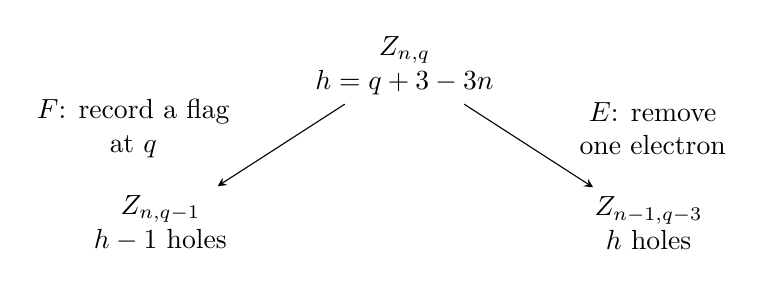
\begin{tikzpicture}[every node/.style={align=center},>=stealth]
 \node (root) at (0,0) {$Z_{n,q}$\\$h=q+3-3n$};
 \node (left) at (-3.1,-2) {$Z_{n,q-1}$\\$h-1$ holes};
 \node (right) at (3.1,-2) {$Z_{n-1,q-3}$\\$h$ holes};
 \draw[->] (root) -- (left);
 \draw[->] (root) -- (right);
 \node[anchor=east] at (-2.1,-0.8) {$F$: record a flag\\at $q$};
 \node[anchor=west] at (2.1,-0.8) {$E$: remove\\one electron};
\end{tikzpicture}
\caption{One step of the orthogonal decomposition.  The displayed spaces
are coordinate spaces for the two branches.  A flag is a record of an
$F$ step; it is not a measured position of a quasihole.}
\label{fig:flags-branches}
\end{figure}

The remaining issue in this decomposition is analytic.  A polar
decomposition need not be local when its nonzero singular values approach
zero.  The next lemma rules out that problem uniformly in the flux.

\subsection{A local polar map}

\begin{lemma}[Occupation gap and local representatives]
\label{lem:flags-polar}
There is $\varepsilon>0$, independent of $q$ and of the number sector,
such that
\begin{equation}
 P_q n_qP_q\geq\varepsilon P_{\mathcal E_q},
 \qquad \mathcal E_q=\bigoplus_n\mathcal E_{n,q}.
 \label{eq:flags-occupation-gap}
\end{equation}
The polar map $\mathsf T_q$ and the projections onto the two branches, restricted
to $Z_q$, have bounded physical representatives rapidly localized at the
south pole.  The representatives preserve $Z_q$ and its orthogonal
complement.  They have respectively the number and index grades of $c_q$
and of the identity.
\end{lemma}

\begin{proof}
We first prove the singular-value bound, keeping track of the restriction
of pair rows.  The normalized rows are
\[
 B_{q,b}=\sum_{\substack{0\leq i<j\leq q\\i+j=b}}
 a_{q,b}(i,j)c_jc_i,\qquad
 a_{q,b}(i,j)=
 \frac{(j-i)\sqrt{\binom qi\binom qj}}
 {\sqrt{q\binom{2q-2}{b-1}}},\quad 1\leq b\leq2q-1.
\]
For completeness, their normalization follows by taking coefficients in
\[
 \sum_{i<j}(j-i)^2\binom qi\binom qj x^{i+j}
 =(1+x)^q(x\partial_x)^2(1+x)^q
  -\bigl((x\partial_x)(1+x)^q\bigr)^2
 =qx(1+x)^{2q-2}.
\]
If a row contains orbital $q$, put $k=2q-b$.  Its removed coefficient
mass is
\[
 p_{q,k}=\frac{k\binom{q-1}{k-1}}{\binom{2q-2}{k-1}}.
\]
Here $p_{q,1}=p_{q,2}=1$, and
\[
 \frac{p_{q,k+1}}{p_{q,k}}
 =\frac{(k+1)(q-k)}{k(2q-k-1)}\leq1.
\]
It follows that every row with a retained pair has retained mass
\begin{equation}
 r_{q,b}=\sum_{\substack{i<j<q\\i+j=b}}|a_{q,b}(i,j)|^2
 \geq\frac{q}{4q-6}\geq\frac14.
 \label{eq:flags-retained-mass}
\end{equation}
Rows with no coefficient at $q$ have mass one.  The two top rows retain
no pair and are omitted.

For $d=1$, the pinning weights obey
$g_j=\tfrac12\log((q-j)/q)$.  Multiplication of its coefficients by
$e^{-g_i-g_j}$, followed by normalization, turns a flux-$(q-1)$ row into
the normalized retained flux-$q$ row.  More precisely, if
$B_{q,b}^{\mathrm{ret}}$ denotes the row with the coefficient at orbital
$q$ deleted, then
$B_{q,b}^{\mathrm{ret}}=\sqrt{r_{q,b}}B_{q,1,b}(1)$, in the notation
of Equation~\eqref{eq:pinning-rows}.  Let $\delta>0$ be the uniform
endpoint gap from Lemma~\ref{pinning:uniform-gap}.  By
\eqref{eq:flags-retained-mass}, the Hamiltonian compressed to the
south-empty sector has a gap at least $\delta/4$ above
$\bigoplus_n\mathcal F_{n,q}$.

The CAR give the exact identity
\[
 \sum_b[B_{q,b},n_q]^*[B_{q,b},n_q]
 =n_q\sum_{k=1}^{q}p_{q,k}n_{q-k}.
\]
The coefficient sum is
\[
 \sum_{k=1}^{q}p_{q,k}=\frac{4q-2}{q+1}<4.
\]
One way to see this is to write
$p_{q,k}=k\binom{2q-k-1}{q-1}/\binom{2q-2}{q-1}$ and apply the
hockey-stick identity twice.  For $\psi\in Z_q$, the two top singleton
rows also imply $c_{q-1}c_q\psi=c_{q-2}c_q\psi=0$.  Hence
\begin{equation}
 \sum_b\|[B_{q,b},n_q]\psi\|^2
 \leq2\|c_q\psi\|^2.
 \label{eq:flags-emptying-energy}
\end{equation}
Let $Q=1-n_q$ and let $P_F$ project onto
$\bigoplus_n\mathcal F_{n,q}$.  Since
$B_{q,b}\psi=0$, the restricted gap gives
\[
 \frac\delta4\|Q\psi-P_F\psi\|^2
 \leq\sum_b\|B_{q,b}Q\psi\|^2
 \leq2\|c_q\psi\|^2.
\]
The occupied and vacant components are orthogonal, so
\[
 \|\psi-P_F\psi\|^2
 \leq(1+8/\delta)\|c_q\psi\|^2.
\]
Thus \eqref{eq:flags-occupation-gap} holds with
$\varepsilon=\delta/(\delta+8)$.

To construct local representatives, take a real smooth frequency cutoff
$\chi$ equal to one near zero and supported strictly inside the uniform
unperturbed gap.  Apply its time filter to $c_q$:
\[
 A_q=\int_{\mathbb R}\widehat\chi(t)
          e^{itH_q}c_qe^{-itH_q}\,dt,
\]
with the Fourier normalization incorporated into $\widehat\chi$.
Contraction preserves zero modes.  The cutoff therefore gives
$A_qP_q=c_qP_q$ and $[A_q,P_q]=0$.  The local calculus makes $A_q$
rapidly localized at the south pole, with uniform constants.  Choose a
smooth function $\eta$ on a fixed interval containing the spectrum of
$A_q^*A_q$, equal to zero near zero and to $x^{-1/2}$ for
$x\geq\varepsilon$.  Then
\[
 \widetilde{\mathsf T}_q=A_q\eta(A_q^*A_q)
\]
is rapidly localized by smooth functional calculus and agrees with
$\mathsf T_q$ on $Z_q$.  Its products
$\widetilde{\mathsf T}_q^*\widetilde{\mathsf T}_q$ and
$1-\widetilde{\mathsf T}_q^*\widetilde{\mathsf T}_q$ represent the branch projections on
$Z_q$.  The construction preserves number and index grades because
$H_q$ preserves both and $A_q^*A_q$ has grade zero.  It also preserves
$P_q$ in both directions.  No claim about a spectral gap of
$A_q^*A_q$ outside $Z_q$ is needed: $\eta$ is smooth on that entire
spectral interval.
\end{proof}

\subsection{One-step comparisons}

Write
\[
 K_{q,d}(f)=\mathcal U_{q,d}^*D_q(f)\mathcal U_{q,d}
              -D_{q-d}(f)
\]
on the corresponding smaller zero space.  Proposition~
\ref{pinning:weighted-transport} supplies localized representatives for
these operators, with the stated size and flux-comparison estimates.

\begin{proposition}[Weighted observable at one branch]
\label{prop:flags-weighted-step}
Fix $p\in(0,2)$, $L\geq2$, and $f(j)=f_{L,p}(j)$.  In the orthogonal
coordinates \eqref{eq:flags-two-branches},
\begin{equation}
 \begin{split}
 (J_{q,F}\oplus J_{q,E})^*D_q(f)(J_{q,F}\oplus J_{q,E})
  ={}&\begin{pmatrix}
   D_{q-1}(f)+K_{q,1}(f)&0\\
   0&D_{q-3}(f)+f(q)+K_{q,3}(f)
  \end{pmatrix}+R_q(f),\\
 &\|R_q(f)\|\leq C_p\frac{f(q)}{(L+q)^2}.
 \end{split}
 \label{eq:flags-weighted-step}
\end{equation}
The notation in the left side means the unitary whose columns are the
two branch isometries.  The bound includes the off-diagonal blocks.
For affine $f$ the remainder is zero and $K_{q,d}(f)=0$.
\end{proposition}

\begin{proof}
The $F$ block is the definition of $K_{q,1}(f)$.  For an affine sequence,
the grades of $\mathsf T_q$ give
\[
 D_q(f)\mathsf T_q=\mathsf T_qD_q(f)-f(q)\mathsf T_q
\]
on the zero spaces, and both branch projections commute with $D_q(f)$.
The endpoint transports commute with the number and index operators.
This proves the affine assertion, including the scalar $f(q)$ in $E$.

For a general $f$, subtract its affine Taylor polynomial at $q$.
The remainder $a(j)=f(j)-f(q)-f'(q)(j-q)$ satisfies
\[
 |a(j)|\leq C_p\frac{f(q)}{(L+q)^2}
                   (1+q-j)^{p+4},\qquad 0\leq j\leq q.
\]
The same polynomial bounds hold for the finite differences needed for
localization.  In the south-pole frame this says that $D_q(a)$ has
one-body interaction size at most $C_pf(q)/(L+q)^2$, times a fixed
polynomial in distance from the pole.  Commuting it with any of the
rapidly localized representatives in Lemma~\ref{lem:flags-polar} thus
has norm at most that size: decompose the representative into ball
shells and sum its arbitrarily high inverse-power tails against this
polynomial.  In the $E$ block use
$\mathsf T_q[D_q(a),\mathsf T_q^*]$; for the off-diagonal blocks use the commutator with
a branch projection.  Compression and the endpoint isometries do not
increase these norms.  This proves \eqref{eq:flags-weighted-step}.
\end{proof}

For a general observable supported far to the north, the polar map
contributes an even smaller error, because its representative is
localized at the opposite pole.  We record the precise form used below.

\begin{lemma}[Northern comparison]
\label{lem:flags-northern-step}
There are fixed $c\geq0$ and $b_0\geq1$ with the following property.
Let $O=O^*$ be neutral, of norm at most one, supported on a slot ball of
radius $r\geq2$ centered at latitude index $m$, and put $u=1+m$.
If $q>C r^{b_0}u$, identify all northern slots in the fluxes being
compared.  The two diagonal branch blocks of $O$ equal
\[
 O+\mathcal D_{q,1}(O)\quad\hbox{and}\quad
 O+\mathcal D_{q,3}(O)
\]
up to a matrix remainder of norm $C_Dq^{-D}$ for every fixed $D$.
Each $\mathcal D_{q,d}(O)$ is neutral and self-adjoint.  If $x$ is its
original center, then, for fixed $c,C_*<\infty$ and every $D>0$,
\begin{equation}
 \begin{split}
 \|\mathcal D_{q,d}(O)\|&\leq Cr^cu/q^2,\\
 \inf_{A_R\in\mathfrak A(B_R(x))}
       \|\mathcal D_{q,d}(O)-A_R\|
  &\leq C_Dr^cu q^{-2}R^{-D}\qquad(R\geq C_*r).
 \end{split}
 \label{eq:flags-northern-size}
\end{equation}
For $|q-q'|\leq2$ and fixed $d$, the difference between these changes,
in common northern slots, obeys the same two estimates with $q^{-2}$
replaced by $q^{-3}$.  The exponent $c$ and core constant $C_*$ are
independent of $D$.
\end{lemma}

\begin{proof}
For $F$, this is Corollary~\ref{pinning:northern-observable}.
Its norm and tail estimates are
Equations~\eqref{eq:pinning-northern-norm} and
\eqref{eq:pinning-northern-tail}; enlarge the fixed core constant to
write the outer ball radius as $R$ instead of $r+R$.
For $E$, commute $O$ through the local representative of $\mathsf T_q$ before
applying that corollary with $d=3$.  The support of $O$ is a distance
comparable with $\sqrt q$ from the south pole when $b_0$ is increased
if necessary.  Rapid locality therefore makes the polar commutator and
the off-branch blocks $O(q^{-D})$ for every $D$.  The same estimate
handles the finitely many trimmed orbitals.  The difference assertion
for the remaining changes is the same-corollary comparison of the
pinning transports at bounded flux difference.
\end{proof}

\subsection{Histories and a linear reference expectation}

Iterate the two branch coordinates until the flux reaches
$q_{\mathrm{stop}}$.  A word $\omega$ records its successive $F$ and
$E$ choices; its terminal number and flux are denoted by $n_\omega$
and $q_\omega$.  The resulting unitary is
\begin{equation}
 \mathcal R_{n,q}:Z_{n,q}\longrightarrow
       \bigoplus_{\omega}Z_{n_\omega,q_\omega}.
 \label{eq:flags-history-map}
\end{equation}
For a fixed readout axis and fixed filters, the maps $J_{q,F}$,
$J_{q,E}$, and $\mathcal R_{n,q}$ are defined on physical Fock spaces
independently of the auxiliary slot frames.  Rebuilding frames outside
the common northern slots changes only the representations used to
prove locality estimates; it does not redefine these maps or their
history coordinates.
An $F$ step taken at flux $b$ records one flag with value $b$.  At a
terminal space we add $q_\omega+3-3n_\omega$ flags, all with value zero.
Let $\mathcal B(\omega)$ be this multiset.  Each word has exactly $h$
flags.  The vacuum follows only $F$ steps, with the same terminal
convention.  We do not resolve the bounded-dimensional terminal space
further.

Fix $a\in(0,2)$.  On the direct sum in
\eqref{eq:flags-history-map}, define the positive diagonal operator
\begin{equation}
 W_m(\omega)=\sum_{b\in\mathcal B(\omega)}
       \min\left\{1,\left(\frac{1+m}{1+b}\right)^a\right\}.
 \label{eq:flags-history-weight}
\end{equation}
Its value is scalar on each terminal summand.  In particular $W_m=0$
on the filled zero space, and $W_m\geq(1+q)^{-a}$ whenever $h>0$.

We next fix the scalar used to center observables.  Put
$q^0=3\lfloor q/3\rfloor$, and let $\Omega_{q^0}$ be the normalized
filled zero mode at that flux.  Embed its one-particle space into $U_q$
by sending orbital $j$ to orbital $j$, and then use the slot embedding
at flux $q$, with the orthogonal complement of the embedded one-particle
space vacant.  Define
\begin{equation}
 \operatorname{ref}_q(O)=
 \langle\Omega_{q^0},O\Omega_{q^0}\rangle
 \label{eq:flags-reference}
\end{equation}
in this padded realization.  This is a positive linear functional of
norm one on the slot algebra.  At $q=q^0$ it is the filled expectation.
For $q^0=0$ the convention is $U_0=\mathbb C$ with its unique normalized
one-electron filled vector.  Outside the common northern region only
linearity, the norm-one bound, and the exact filled expectation at
$q=q^0$ will be used.

\begin{lemma}[Compatibility of reference expectations]
\label{lem:flags-reference-compatibility}
Let two fluxes $q,q'$ use common northern slots, and let
$s\leq\min(q,q')$.  Embed a fixed vector of $\mathcal F_s$ into either
system by the same orbital labels, with the orthogonal complement of
the embedded one-particle space vacant.  The two states have identical
expectations on the algebra of common northern slots.  In particular,
references at fluxes with the same nearest lower filled flux agree on
that algebra.
\end{lemma}

\begin{proof}
Expand a slot observable into normally ordered CAR monomials.  Its
expectation in an embedded state is a linear combination of the state's
normally ordered orbital correlations.  The coefficients use only the
analysis-frame entries of the slots occurring in the monomial.  Entries
at orbital labels above $s$ contribute zero, because those orbitals are
vacant.  At labels at most $s$, the common northern frame entries are
identical.  Thus every monomial has the same expectation in both
realizations.  This also proves the assertion after physical compression
of the slot observable, which leaves these matrix elements unchanged.
\end{proof}

The parent and its $E$ child use filled states at $q^0$ and $q^0-3$,
respectively.  Their expectations are related by the filled $E$ step.
By contrast, the references at $q-3$ and $q^0-3$ use the same filled
state and agree on common northern slots by
Lemma~\ref{lem:flags-reference-compatibility}.  For a rapidly localized
operator, apply this exact identity to a truncation supported in those
slots; the remaining difference is at most twice the truncation error.
The common-frame construction permits these conventions for every
frame entering a comparison, with uniform estimates.

\begin{theorem}[Local observables in history coordinates]
\label{thm:flags-local-readout}
For every fixed $a\in(0,2)$ there are $B,C<\infty$ such that the
following holds uniformly in $n,q$ and in the allowed slot frames.
Let $O=O^*$ be a neutral slot observable of norm at most one, supported
in a ball of radius $r\geq2$ with center of latitude index $m$.  Its
compression to $Z_{n,q}$ satisfies
\begin{equation}
 \pm\left(
 \mathcal R_{n,q}P_{n,q}OP_{n,q}\mathcal R_{n,q}^*
       -\operatorname{ref}_q(O)I\right)
 \leq C r^B W_m.
 \label{eq:flags-local-readout}
\end{equation}
Here $P_{n,q}$ denotes the zero-space projection in the number-$n$
sector.  More generally, for a convergent decomposition
$A=\sum_\nu A_\nu$ into neutral self-adjoint observables supported in
balls about the same center, of respective radii $r_\nu\geq2$, the
right side can be replaced by
$CW_m\sum_\nu r_\nu^B\|A_\nu\|$.
\end{theorem}

\begin{proof}
The proof keeps $O$ unchanged while descending through common northern
slots.  Only the small changes caused by each transport are estimated
inductively.  This distinction prevents an increasing radius from
being assigned repeatedly to the original observable.

We first describe the centered one-step identities under the northern
condition of Lemma~\ref{lem:flags-northern-step}.  For an $E$ step
put $t=q-3$, so $t^0=q^0-3$, and write $R_{q,E}(O)$ for its uncentered
polar remainder in Lemma~\ref{lem:flags-northern-step}.  The filled
$E$ step at $q^0$, together with compatibility of the northern
references, gives the exact scalar identity
\[
 \operatorname{ref}_q(O)-\operatorname{ref}_t(O)
 =\operatorname{ref}_{t^0}\bigl(
     \mathcal D_{q^0,3}(O)+R_{q^0,E}(O)\bigr).
\]
Thus the parent-to-child reference change is determined by a filled
step.  Define
\[
 \begin{split}
 R_{q,E}'(O)&=R_{q,E}(O)
           -\operatorname{ref}_{t^0}(R_{q^0,E}(O))I,\\
 s_q(O)&=\operatorname{ref}_t(\mathcal D_{q,3}(O))
         -\operatorname{ref}_{t^0}(\mathcal D_{q^0,3}(O)).
 \end{split}
\]
The references in the second line use the same filled state.
Lemma~\ref{lem:flags-reference-compatibility}, first on common northern
slots and then on rapid tails by norm approximation, therefore gives
\[
 s_q(O)=\operatorname{ref}_{t^0}\bigl(
     \mathcal D_{q,3}(O)-\mathcal D_{q^0,3}(O)\bigr)
     +O(q^{-D}).
\]
The bounded-flux comparison in Lemma~\ref{lem:flags-northern-step}
supplies the additional factor $q^{-1}$.  Substituting these scalar
identities into the branch comparison yields
\begin{equation}
 \begin{split}
 J_{q,E}^*(O-\operatorname{ref}_q(O))J_{q,E}
 ={}&(O-\operatorname{ref}_t(O))
    +\bigl(\mathcal D_{q,3}(O)
               -\operatorname{ref}_t(\mathcal D_{q,3}(O))\bigr)\\
    &+s_q(O)I+R_{q,E}'(O),\\
 |s_q(O)|\leq{}&Cr^c u/q^3+C_Dq^{-D},\qquad
 \|R_{q,E}'(O)\|\leq C_Dq^{-D}.
 \end{split}
 \label{eq:flags-centered-E}
\end{equation}
Here and below the symbols denote compressions to the relevant child
zero space.  When $h=0$ the comparison is its own filled calibration,
so all centered contributions vanish exactly.

For an $F$ step, $t=q-1$.  The nearest smaller filled fluxes are either
identical or differ by three.  In the latter case apply the filled
$E$ comparison just used.  Together with
\eqref{eq:flags-northern-size}, this proves
\begin{equation}
 J_{q,F}^*(O-\operatorname{ref}_q(O))J_{q,F}
 =O-\operatorname{ref}_t(O)+S_{q,F}(O),\qquad
 \|S_{q,F}(O)\|\leq Cr^cu/q^2+C_Dq^{-D}.
 \label{eq:flags-centered-F}
\end{equation}
The off-diagonal blocks have norm $C_Dq^{-D}$.  An $F$ step already
records a flag, so its entire error will be charged to that flag.

Here is a uniform closure argument, including the parameter choices.
Let $c,b_0$ be as in Lemma~\ref{lem:flags-northern-step}.  Choose
$b>\max\{b_0,c\}$, then choose $B>\max\{ab,c\}$ large enough to
absorb the fixed polynomial costs of the local calculus.  A constant
$M$ will be fixed after $B$.  Set
\[
 \tau=Mr^b u.
\]
If $q\leq\tau$ and $h>0$, every flag has $b'\leq q$, so
\[
 W_m\geq(2Mr^b)^{-a}I.
\]
The norm bound $\|O-\operatorname{ref}_q(O)\|\leq2$ proves
\eqref{eq:flags-local-readout} in this region with constant
$2(2M)^a$.  When $h=0$ the centered compression is zero.  Increasing
$M$ includes all stopping cases in this argument.

Fix a finite $Q$, and let $K_Q$ be the least constant in
\eqref{eq:flags-local-readout} for fluxes at most $Q$, with the
chosen $B$, all number sectors, and all allowed frames.  This number
is finite: for $h>0$ use $W_m\geq(1+Q)^{-a}$, while the filled
compression is exactly centered.  We prove
\begin{equation}
 K_Q\leq C_M+\frac12K_Q
 \label{eq:flags-bootstrap-constant}
\end{equation}
with $C_M$ independent of $Q$.

Suppose $q>\tau$.  Expand the unchanged $O$ down the branching tree,
using \eqref{eq:flags-centered-E} and
\eqref{eq:flags-centered-F}, until the current flux is at most
$\tau$.  The original northern slots, center, and radius are unchanged
through this part of the descent.  The terminal comparisons have just
been bounded.  In an $E$ child, decompose
$\mathcal D_{q,3}(O)$ into its core and dyadic ball shells, all centered
at $m$.  Equation~\eqref{eq:pinning-northern-moment}, with a tail order
larger than $B+2$, gives
\[
 \sum_\nu r_\nu^B\|\mathcal D_{q,3}(O)_\nu\|
 \leq C(B)r^{B+c}u/q^2.
\]
Applying the definition of $K_Q$ to each smaller-flux shell, and using
linearity of the reference, bounds its centered contribution by
\[
 K_QC(B)r^{B+c}u/q^2
\]
times the remaining history weight in that child.  Along any word,
the flux strictly decreases; thus
\[
 \sum_{q'>\tau}\frac{u}{(q')^2}\leq C\frac{u}{\tau}
       =\frac{C}{Mr^b}.
\]
Consequently all induction-dependent contributions are bounded by
\[
 K_Q\frac{C(B)}M r^{B+c-b}W_m.
\]
Choose $M$ so large that this is at most
$\tfrac12 K_Qr^BW_m$.  This choice is possible because $b>c$ and
$r\geq2$.

We verify that the other errors have a bound independent of $K_Q$.
At a node with positive remaining hole number, its identity is bounded
by the sum of the identities assigned to its remaining flags.  A
scalar electron error may therefore be charged to every such flag.
For a flag at $\ell$, the total charge from ancestors in
\eqref{eq:flags-centered-E} is at most
\begin{equation}
 C\frac{r^cu}{\max\{\tau,1+\ell\}^2}.
 \label{eq:flags-scalar-tail}
\end{equation}
The $F$ error in \eqref{eq:flags-centered-F} occurs at its own flag
and obeys the same bound, up to a fixed constant.  Write
$w_\ell=\min\{1,(u/(1+\ell))^a\}$.  Since $a<2$ and $\tau=Mr^bu$,
\[
 \frac{r^cu}{\max\{\tau,1+\ell\}^2}
 \leq C M^{a-2}r^{c+b(a-2)}w_\ell
 \leq C_M r^B w_\ell.
\]
The $q^{-D}$ remainders, including the off-diagonal blocks, obey the
same estimate after choosing $D>a+2$.  For a self-adjoint off-diagonal
block, its norm bounds the full block matrix above and below by that
norm times the identity at its node, so the same charge applies.
Nodes with $h=0$ contribute nothing, by the exact centered filled
identity.  Summation of these diagonal bounds along words proves
\eqref{eq:flags-bootstrap-constant}.

It follows that $K_Q\leq2C_M$ for every $Q$, proving the uniform
claim.  Finally, the assertion for $A=\sum_\nu A_\nu$ follows by
linearity of the reference and by summing the form inequalities.
\end{proof}

The theorem estimates a compression to the zero spaces.  It does not
claim that ordinary local fluctuations vanish in the filled state.
It also applies to coherent superpositions of histories: all charges
above are diagonal operator bounds, rather than bounds conditional on
a classical choice of word.

\subsection{Rotation averaging in a one-hole space}

The history estimate still depends on a chosen readout axis.  In this
subsection, a one-hole space means a space with quasihole degree $h=1$.
Representation theory then removes the axis dependence and yields an
integrated estimate with no factor of the sphere area.

\begin{corollary}[One-hole comparison]
\label{cor:flags-one-hole}
Suppose $h=1$, equivalently $q=3n-2$.  Let $\psi,\phi$ be any two unit
vectors in $Z_{n,q}$.  Let $\{O_x\}$ be a measurable family of neutral
self-adjoint observables of norm at most one, supported in balls of a
fixed radius $r\geq2$ about $x$, with center measure of bounded density.
There are constants $C,B'<\infty$, independent of $n,q$, such that
\begin{equation}
 \int\left|
 \langle\psi,O_x\psi\rangle-\langle\phi,O_x\phi\rangle
 \right|\,dx\leq Cr^{B'}.
 \label{eq:flags-one-hole}
\end{equation}
The same conclusion holds for rapidly localized families, with the
right side bounded by the corresponding fixed rapid-locality seminorm.
For a family whose norms are bounded by $A$, multiply the right side by
$A$.
\end{corollary}

\begin{proof}
Choose $a\in(1,2)$ in Theorem~\ref{thm:flags-local-readout}.  The
symmetric-polynomial factor in \eqref{eq:flags-polynomial-space} has
degree one in each variable.  It is the irreducible spin-$n/2$
representation, so $Z_{n,q}$ is irreducible and has dimension $n+1$.

When $h=1$, an $F$ branch has $h=0$ and hence dimension one.  Before
that branch all steps are $E$, which lower the flux by three.
Therefore at most one one-dimensional history has a flag at any
specified nonterminal flux.  The history that reaches the stopping
region without an $F$ step has bounded terminal dimension.  It follows
that, as an operator on $Z_{n,q}$,
\begin{equation}
 \operatorname{Tr}(W_0)
 \leq C+\sum_{b\geq0}(1+b)^{-a}\leq C_a.
 \label{eq:flags-one-hole-trace}
\end{equation}
The trace is unchanged on conjugating back to the physical zero space.
Write $\widehat W_0=\mathcal R_{n,q}^*W_0\mathcal R_{n,q}$ for that
physical operator.

Let $V_q(g)$ denote the rotation representation, with normalized Haar
measure $dg$.  Schur's lemma gives
\[
 \int_{\mathrm{SU}(2)}V_q(g)\widehat W_0V_q(g)^*\,dg
 =\frac{\operatorname{Tr}(\widehat W_0)}{n+1}I.
\]
For each rotation use the readout axis whose north pole is the image
of the original north pole.  Precisely, write
$x(g)=g\cdot\mathrm{north}$ and
$W^{g}=V_q(g)\widehat W_0V_q(g)^*$.
Use the rotated frame and rotated branch construction at $x(g)$.
Theorem~\ref{thm:flags-local-readout}, applied to $O_{x(g)}$, gives
\[
 \bigl|\langle\psi,O_{x(g)}\psi\rangle
       -\langle\phi,O_{x(g)}\phi\rangle\bigr|
 \leq Cr^{B'}\bigl(\langle\psi,W^g\psi\rangle
                    +\langle\phi,W^g\phi\rangle\bigr).
\]
The two reference expectations cancel in this inequality.
Changes between local frames cost only a fixed polynomial in $r$ by
the local calculus.  Integrating rotations and multiplying by the
sphere area yields at most
$Cr^{B'}q\operatorname{Tr}(W_0)/(n+1)$, which is uniformly bounded
because $q=3n-2$.  For any center measure with bounded mass in unit
balls, spread the mass at each center over a ball of fixed radius.
The resulting density relative to area is bounded uniformly.  The
operator originally assigned to $x$ is supported in a ball of radius
$r+1$ about every point in that spreading ball, so the same pointwise
bound applies before integration.  This reduces the general center
measure to the area estimate.  Finally, summing ball shells proves the
assertion for rapid families.
\end{proof}

\section{Charge bounds and rotation averaging}
\label{sec:charge}

The history estimate of Theorem~\ref{thm:flags-local-readout} controls a
local observable by weighted flags.  To treat arbitrary hole number by
rotation averaging, we compare these weights with a physical one-body
observable, first with a slowly decreasing weight and then with a
summable weight.

Increase the fixed stopping flux in the history construction, if
necessary, so that it is at least eight and all pinning comparisons
above it are valid, including shifts by at most three.  Write
$q_{\rm s}=q_{\mathrm{stop}}$ and let $\mathcal R_{n,q}$ denote
the history unitary in \eqref{eq:flags-history-map}.  For $L\ge2$ and
$0<p<2$, put
\begin{equation}\label{eq:charge-definitions}
 \begin{gathered}
 f(x)=f_{L,p}(x)=\left(\frac{L}{L+x}\right)^p,\qquad
 C_q(f)=\frac{q+3}{3(q+1)}\sum_{j=0}^q f(j),\\
 S_{L,p}(\omega)=\sum_{b\in\mathcal B(\omega)}f(b).
 \end{gathered}
\end{equation}
When $q$ is divisible by three, $C_q(f)$ is the filled-state expectation
of $D_q(f)$: rotational invariance gives occupation
$(q+3)/(3(q+1))$ in every orbital.  The formula defines the scalar
$C_q(f)$ also at the other fluxes.  The operator $S_{L,p}$ is diagonal
in histories and scalar on each terminal summand.  Its sum is over the
flag multiset $\mathcal B(\omega)$, including all terminal flags at
position zero; each history has exactly $h=q+3-3n$ flags.  All operator
inequalities involving $S_{L,p}$ below are in history coordinates.  In particular, they make no measurement
assumption about flags in a zero-mode vector.

\begin{proposition}[Pooled charge]\label{prop:charge-pooled}
For each of $p=1/8$ and $p=3/2$ there are fixed $L\ge2$ and $c>0$ such
that, for every flux and every nonzero zero-mode space $Z_{n,q}$,
\begin{equation}\label{eq:charge-pooled}
 \mathcal R_{n,q}\bigl(C_q(f)\mathbf1-P_{n,q}D_q(f)P_{n,q}\bigr)\mathcal R_{n,q}^*
 \ \ge\ c S_{L,p}.
\end{equation}
Here compression to $Z_{n,q}$ is understood, and $P_{n,q}$ denotes its
orthogonal projection.  The constants are independent of $q,n$ and of
the readout axis.  When $h=0$, both sides vanish.
\end{proposition}

The obstruction to this estimate occurs at electron steps.  Along a
history, each F step contributes approximately $-f(q)/3$ to
$D_q(f)-C_q(f)\mathbf1$, supplying a credit for its new flag.  Each E
step contributes a positive scalar correction.  When at least two
flags remain, divide this scalar cost between them.  The scalar tail
estimate below leaves the strictly positive margin
\[
 \frac13-\frac{1+p}{6(1-p)}=\frac5{42}\qquad(p=1/8).
\]
With one remaining flag, there is no such margin.  We instead combine
the scalar with the transported observable and compare it to a filled
step; the one-hole comparison of Corollary~\ref{cor:flags-one-hole}
makes the resulting error summably small.  These two cases prove the
first charge estimate.

Rotation averaging then bounds integrated local-expectation differences
between two zero-mode states by $C(q+1)^{7/8}$ times the sum of their
hole numbers.  This still grows with the
area, but it is enough to prove the charge estimate again with $p=3/2$.
For a polar annulus $1+m\asymp M$, use this averaged bound while the
flux is moderate relative to $M$; the transport interaction has a
factor $(q+1)^{-2}$ that pays for the area dependence.  At larger
flux, apply the original fixed-axis history estimate directly to the
annulus.  The two resulting sums are small when the new weight scale
$L$ is large.  The summable weight then gives the area-independent
local-expectation bound at the end of this section.

\subsection{Scalar telescoping and summable error bounds}

We estimate $D_q(f)-C_q(f)\mathbf1$ from above.  An F step contributes
the scalar $C_{q-1}(f)-C_q(f)$, and an E step contributes
\begin{equation}\label{eq:charge-electron-scalar}
 \ell_q=C_{q-3}(f)+f(q)-C_q(f).
\end{equation}
For the continuous comparison define
\begin{equation}\label{eq:charge-continuous-scalar}
 F(x)=\frac1x\int_0^x f(t)\,dt,\qquad
 \ell(x)=-2F'(x)+f'(x)\quad(x>0),
\end{equation}
with the continuous extensions at zero.

\begin{lemma}[Scalar estimates]\label{lem:charge-scalars}
Fix $p\in(0,2)$ and a lower stopping flux $q_{\rm s}\ge8$.  There is a
function $\varepsilon_p(L)\to0$ as $L\to\infty$ with the following
properties, uniformly for $q\ge q_{\rm s}$:
\begin{align}
 \left|C_{q-1}(f)-C_q(f)+\frac13f(q)\right|
 &\le\varepsilon_p(L)f(q),\label{eq:charge-F-scalar}\\
 \sum_{q\ge q_{\rm s}}
 \frac{|\ell_q-\ell_{3\lfloor q/3\rfloor}|}{f(q)}
 &\le\varepsilon_p(L).\label{eq:charge-calibration-scalar}
\end{align}
The function $\ell$ is nonnegative.  If $0<p<1$, then for every
collection $\mathcal E$ of E-step fluxes along a history, and every
flag position $k$ below these steps,
\begin{equation}\label{eq:charge-scalar-tail}
 \sum_{\substack{q\in\mathcal E\\q\ge k}}(\ell_q)_+
 \le \left(\frac{1+p}{3(1-p)}+\varepsilon_p(L)\right)f(k).
\end{equation}
Changing $k$ by a fixed bounded amount, or taking $k$ in the terminal
range, only changes $\varepsilon_p(L)$.
\end{lemma}

\begin{proof}
The exact formula
\begin{equation}\label{eq:charge-scalar-exact}
 \ell_q=f(q)-\left(1+\frac2{q+1}\right)
 \frac{f(q)+f(q-1)+f(q-2)}3
 +\frac{2\sum_{j=0}^{q-3}f(j)}{(q+1)(q-2)}
\end{equation}
is obtained by separating the last three summands in $C_q$.
A useful positive form of this identity is obtained by putting
$d_j=f(j)-2f(j+1)+f(j+2)$ and $Q_q=(q+1)(q-2)$:
\begin{equation}\label{eq:charge-positive-scalar}
 \ell_q=\frac1{Q_q}\sum_{j=0}^{q-3}(j+1)(j+2)d_j
       +\frac{2q}{3(q+1)}d_{q-2}.
\end{equation}
Expanding the second differences verifies the formula coefficient by
coefficient.  In particular, $\ell_q\ge0$, and constant and affine
functions contribute zero.

Here are precise discrete-to-continuous error bounds:
\begin{align}
 |\ell_q-\ell(q)|+
 \sup_{x\in[q-3,q]}|\ell(x)-\ell(q)|
 &\le C(L+q)^{-2},\label{eq:charge-scalar-errors}\\
 |\ell_q-\ell_{q-r}|
 &\le
 \begin{cases}
 C L^{-2},&q\le L,\\
 C(F(q)+f(q))q^{-2},&q>L,
 \end{cases}\label{eq:charge-scalar-differences}
\end{align}
for $r=0,1,2$.  We give details because the sharper second estimate is
needed for the summable weight.  The identity
$d_j=\int (1-|t-j-1|)_+f''(t)\,dt$ expresses
\eqref{eq:charge-positive-scalar} as $\int_0^q \kappa_q(t)f''(t)\,dt$.
The function $\kappa_q$ is linear between consecutive integers and has values
\[
 \kappa_q(i)=\frac{i(i+1)}{Q_q}\ (0\le i\le q-2),\qquad
 \kappa_q(q-1)=\frac{2q}{3(q+1)},\qquad \kappa_q(q)=0.
\]
On $[0,q-2]$ its difference from $t^2/q^2$ is at most
$C(t/q^2+t^2/q^3)$, and on $[q-2,q]$ that difference is bounded by a
constant.  The error in its integral against $f''$ is consequently at
most
\[
 C\left(q^{-2}\int_0^q tf''(t)\,dt+
 q^{-3}\int_0^q t^2f''(t)\,dt+
 \int_{q-2}^q f''(t)\,dt\right).
\]
For $q\le L$ use $f''\le C/L^2$; for $q>L$ use
$\int_0^q tf''\le1$, $\int_0^q t^2f''\le2qF(q)$, and
$f''(t)\le C f(t)(L+t)^{-2}$.  This proves the first term of
\eqref{eq:charge-scalar-errors}.  The continuous identity
$\ell(x)=x^{-2}\int_0^x t^2f''(t)\,dt$ implies
$\ell'(x)=f''(x)-2\ell(x)/x$, which proves the oscillation estimate.

For \eqref{eq:charge-scalar-differences}, difference the positive
formula directly:
\[
\begin{split}
 \ell_q-\ell_{q-1}
 ={}&-\frac{2(q-1)}{Q_qQ_{q-1}}
      \sum_{j=0}^{q-4}(j+1)(j+2)d_j\\
 &+\frac{(q-1)(q-2)}{3q(q+1)}d_{q-3}
  +\frac{2q}{3(q+1)}d_{q-2}.
\end{split}
\]
The first sum is bounded by $CqF(q)$, as follows by its integral
representation and $\int_0^q t^2f''\le2qF(q)$.
This gives $CF(q)/q^2$ when $q>L$; the last two terms cost
$Cf(q)/q^2$.  Below $L$ use $d_j\le C/L^2$ in the displayed
formula.  A bounded number of differences proves the claimed bound.

The exact F-step identity is
\[
 C_{q-1}(f)-C_q(f)+\frac13 f(q)
 =\frac{2}{3q(q+1)}\sum_{j=0}^{q-1}\bigl(f(j)-f(q)\bigr).
\]
For $q\le L$ its ratio to $f(q)$ is $O(L^{-1})$.  For $q>L$ use
\begin{equation}\label{eq:charge-average-weight}
 F(q)\le
 \begin{cases}
 f(q)/(1-p),&p<1,\\
 C_pL/q,&p>1.
 \end{cases}
\end{equation}
The resulting ratio is $O(L^{-1})$ also when $1<p<2$, since
$L^{1-p}q^{p-2}\le L^{-1}$ for $q\ge L$.
The case $p=1$ follows from the explicit logarithmic integral and is
not needed below.  Dividing \eqref{eq:charge-scalar-differences} by
$f(q)$ and summing gives $O(L^{-1})$ below $L$.  Above $L$ it
gives $O(L^{-1})$: the summands are $O(q^{-2})$ for $p<1$ and
$O(q^{-2}+L^{1-p}q^{p-3})$ for $1<p<2$.

Twice integrating $f''$ proves
\[
 \ell(x)=\frac1{x^2}\int_0^x t^2f''(t)\,dt\ge0,
 \qquad
 \int_k^\infty\ell(x)\,dx=2F(k)-f(k).
\]
The E-step intervals $[q-3,q]$ have disjoint interiors along a history.
Consequently their continuous contribution is at most
$\frac13\int_{(k-3)_+}^{\infty}\ell(x)\,dx$.
For $p<1$, \eqref{eq:charge-average-weight} bounds this by
$\frac{1+p}{3(1-p)}f(k)$, up to $O(L^{-1})f(k)$ from the bounded
endpoint shift.  Finally, the tail sum of
\eqref{eq:charge-scalar-errors} is bounded by $C/(L+k)$, and
\[
 \frac1{L+k}\le\frac1L f(k)\qquad(0<p<1).
\]
Thus it is $O(L^{-1})f(k)$ uniformly in $k$.
This proves \eqref{eq:charge-scalar-tail}.
\end{proof}

We next list the analytic error sums that will be used in both charge
arguments.  Retain the size function $A_q$ from
Proposition~\ref{pinning:weighted-transport}.  With $u=1+m$,
$v=1+q-m$, and $w=\sqrt{uv/(q+1)}$, it satisfies
\begin{equation}\label{eq:charge-size}
 \begin{gathered}
 A_q(m)=\frac{u^2f''(m)}{(q+1)^2}
 \asymp\frac{f(m)}{(q+1)^2}\left(\frac{u}{L+u}\right)^2,\\
 B_q=\int_0^q A_q(m)\,dm,\qquad
 J_q=\int_0^q\frac{A_q(m)}v\,dm.
 \end{gathered}
\end{equation}
The longitude integral has bounded mass and is included in constants.
Proposition~\ref{pinning:weighted-transport} gives this size for each
transported change in $D(f)$.

\begin{lemma}[Uniform error sums]\label{lem:charge-sums}
For either $p=1/8$ or $p=3/2$, as $L\to\infty$,
\begin{equation}\label{eq:charge-common-sums}
 \sup_{q\ge q_{\rm s}}\frac{B_q}{f(q)}=O(L^{-1}),\qquad
 \sum_{q\ge q_{\rm s}}
 \left(\frac{J_q}{f(q)}+\frac1{(L+q)^2}\right)
 =O\left(\frac{1+\log L}{L}\right).
\end{equation}
For $p=1/8$ there are, in addition,
\begin{equation}\label{eq:charge-first-sums}
 \sum_{q\ge q_{\rm s}}
 \frac{\sup_{0\le m\le q}A_q(m)}{f(q)}=O(L^{-1}),\qquad
 \sum_{q\ge q_{\rm s}}\frac1{f(q)}
 \int_0^q\frac{A_q(m)}w\,dm=O(L^{-1/2}).
\end{equation}
All implied constants are independent of $L$.
\end{lemma}

\begin{proof}
For $q\le L$, integrating $u^2/L^2$ gives
$B_q\le C(q+1)L^{-2}$; for $q>L$, dropping the factor
$(u/(L+u))^2$ gives $B_q\le C F(q)/q$.
These estimates and \eqref{eq:charge-average-weight} prove the first
bound in \eqref{eq:charge-common-sums}.
On the northern half of the sphere $v\ge(q+1)/2$, whereas on the
southern half $A_q(m)\le C f(q)(L+q)^{-2}$.  Therefore
\[
 \frac{J_q}{f(q)}\le
 \frac{C B_q}{(q+1)f(q)}+
 \frac{C\log(q+2)}{(L+q)^2}.
\]
The first term sums to $O(L^{-1})$: above $L$ it is bounded by
$Cq^{-2}$ for $p<1$ and by $CL^{1-p}q^{p-3}$ for $p>1$.
The second sums to $O((1+\log L)/L)$.

For the supremum in \eqref{eq:charge-first-sums}, use $CL^{-2}$
when $q\le L$ and $C(q+1)^{-2}$ otherwise.  The latter divided by
$f(q)$ is $O(L^{-p}q^{p-2})$, whose sum is $O(L^{-1})$ for $p<1$.
On the northern half, $w\ge c\sqrt u$, so the last integral is at
most
\[
 \frac{C}{(q+1)^2}\int_0^{q/2}
 \frac{f(m)u^{3/2}}{(L+u)^2}\,dm
 +\frac{C\sqrt{q+1}\,f(q)}{(L+q)^2}.
\]
After division by $f(q)$, both terms are bounded by
$C\sqrt{q+1}/L^2$ for $q\le L$ and by $Cq^{-3/2}$ for $q>L$,
provided $p<1/2$.  Their sums are $O(L^{-1/2})$.
\end{proof}

\subsection{Calibration and the first charge estimate}

Set $K_q:=K_{q,3}(f)$ on $\mathcal F_{q-3}$.  Its compression to
$Z_{n-1,q-3}$ is the transported change in an E step from $Z_{n,q}$,
as in Proposition~\ref{prop:flags-weighted-step}.  Its center terms
have size $A_q(m)$.  A direct estimate of $\ell_q$ would accumulate a scalar
even in a filled state.  We instead calibrate $K_q+\ell_q$ by a
filled step at the nearest lower flux divisible by three.

Put $q^0=3\lfloor q/3\rfloor$ and $r=q-q^0\in\{0,1,2\}$.
Start with the filled state at flux $q^0-3$ and increase the flux
$r$ times by F transport at the same south pole.  The resulting unit
vector $\chi_q$ lies at flux $q-3$ and has the minimum possible hole
number $r$.  If $r=0$, it is the filled state itself.

\begin{lemma}[Calibrated electron step]\label{lem:charge-calibration}
For $q$ above the fixed stopping range,
\begin{equation}\label{eq:charge-calibrated-scalar}
 \left|\ell_q+\langle K_q\rangle_{\chi_q}\right|
 \le C\left(J_q+|\ell_q-\ell_{q^0}|
              +\frac{f(q)}{(L+q)^2}\right).
\end{equation}
For any collection of northern center terms of $K_q$, their expectation
in $\chi_q$ may instead be replaced by the linear reference functional
of Theorem~\ref{thm:flags-local-readout} at child flux $q-3$; the
additional error is at most $CJ_q$.  This remains true when the choice between the two centerings
is made separately on disjoint annuli.
\end{lemma}

\begin{proof}
In the filled E step at $q^0$, both parent and child compressions of
$D(f)-C(f)\mathbf1$ vanish.  Proposition~\ref{prop:flags-weighted-step}
therefore gives
$|\ell_{q^0}+\langle K_{q^0}\rangle|\le
C f(q^0)(L+q^0)^{-2}$.
Corollary~\ref{pinning:calibration-cost} compares this filled-step
expectation first with the directly embedded lower-flux state and then
with its at most two F-growth transports.  Its bound is $CJ_q$ for
each comparison, proving \eqref{eq:charge-calibrated-scalar} after
adding $|\ell_q-\ell_{q^0}|$.

For a northern source center, the linear reference functional of
Theorem~\ref{thm:flags-local-readout}, applied at child flux $q-3$, is
the expectation in the same directly embedded filled state at $q^0-3$,
using the common slots.
The last assertion of Corollary~\ref{pinning:calibration-cost} applies
to any selected collection of source pieces and bounds the sum of
absolute comparison errors by $CJ_q$.  It therefore also permits the
annulus-dependent choice of centering in the statement.
\end{proof}

For completeness, the elementary rule for summing history bounds is
as follows.  At a node of flux $q$ with positive hole number, every
descendant flag is at an index at most $q$, and hence
\begin{equation}\label{eq:charge-node-lower-bound}
 S_{L,p}\ge h f(q)\mathbf1\ge f(q)\mathbf1
\end{equation}
on that node's full descendant space.  A node error bounded by
$\eta_q f(q)\mathbf1$ can consequently be replaced by
$\eta_q S_{L,p}$ there.  If $\sum_q\eta_q\le\eta$, the sum of all
these node errors is at most $\eta S_{L,p}$: on each history, each
flag appears only at ancestor fluxes, each visited at most once.
This is a comparison of diagonal operators after the node form
bounds have been applied.  It also controls an off-diagonal
remainder by its operator norm.  At a node with no holes, use the
exact vanishing of the centered compression instead of this rule.

\begin{proof}[Proof of Proposition~\ref{prop:charge-pooled} for $p=1/8$]
Apply Proposition~\ref{prop:flags-weighted-step} recursively to
$D_q(f)-C_q(f)\mathbf1$.  The norm remainder at a node is at most
$C f(q)(L+q)^{-2}$, and its total cost is $o_L(1)S_{L,p}$ by
\eqref{eq:charge-node-lower-bound} and
Lemma~\ref{lem:charge-sums}.  F transport has norm at most $CB_q$.
Together with \eqref{eq:charge-F-scalar}, its contribution is
\[
 -\bigl(\tfrac13-o_L(1)\bigr)f(q)
\]
for the flag created at that step.

At an E step with one remaining hole, $q\equiv1\pmod3$, so $\chi_q$
also has one hole.  Compare the child vector to $\chi_q$ using Corollary~\ref{cor:flags-one-hole}.
The difference of the $K_q$ expectations is at most
$C\sup_m A_q(m)$.  This is a two-sided form bound since it holds
for every unit vector in the child space.  The calibration error
and all one-hole errors have total cost $o_L(1)S_{L,p}$ by
Lemmas~\ref{lem:charge-scalars} and \ref{lem:charge-sums}.

At an E step with at least two remaining holes, Proposition~\ref{pinning:one-sided}
bounds the increase from $K_q$ by
$C\int A_q(m)/w\,dm$.  Its total cost is again $o_L(1)S_{L,p}$.
It remains to pay the positive part of $\ell_q$.
Divide that scalar equally among the remaining flags.  A fixed flag
then pays at most one half of each $(\ell_q)_+$ at such an ancestor.
The E-step intervals are disjoint, so
Lemma~\ref{lem:charge-scalars} bounds the total payment for a flag at
$k$ by
\[
 \left(\frac{1+p}{6(1-p)}+o_L(1)\right)f(k)
 =\bigl(\tfrac3{14}+o_L(1)\bigr)f(k).
\]

At terminal fluxes there are only finitely many spaces.  Uniformly
on them, $f(j)=1+O(L^{-1})$, and hence
\[
 D_q(f)-C_q(f)\mathbf1=-\frac h3\mathbf1+O(L^{-1}).
\]
For $h=0$ the expression is exactly zero by rotational invariance;
for $h\ge1$ the error is $O(L^{-1})h$, which is also
$O(L^{-1})$ times the terminal flag weight.  Terminal flags
therefore receive the same credit $1/3-o_L(1)$.
Combining all bounds yields
\[
 \mathcal R_{n,q}(D_q(f)-C_q(f)\mathbf1)\mathcal R_{n,q}^*
 \le-\bigl(\tfrac13-\tfrac3{14}-o_L(1)\bigr)S_{L,p}.
\]
The strict margin is $5/42$.  Choose $L=L_0$ so that the total error
is less than $5/84$ and take $c=5/84$.
\end{proof}

We record what this first estimate gives after rotation averaging.
It will be applied to annular portions of the next transport
interaction, with their center size factored out.

\begin{corollary}[First averaged comparison]\label{cor:charge-weak-average}
Let $W$ be a neutral Hermitian interaction with bounded strength per
unit area and fixed rapid locality bounds.  For unit vectors
$\psi\in Z_{n,q}$ and $\chi\in Z_{n',q}$ with hole numbers $h,h'$,
\begin{equation}\label{eq:charge-weak-average}
 |\langle W\rangle_\psi-\langle W\rangle_\chi|
 \le C_W(q+1)^{7/8}(h+h').
\end{equation}
For radius-$r$ interactions of unit local norm one can take
$C_W\le C(1+r)^B$ for a fixed $B$.
\end{corollary}

\begin{proof}
To specify the rotation average on a physical zero space, let
$V_{n,q}(g)$ denote its rotation representation and define
\[
 S_{L,p}^{g}=V_{n,q}(g)\mathcal R_{n,q}^*S_{L,p}
             \mathcal R_{n,q}V_{n,q}(g)^*.
\]
Thus $S_{L,p}^{g}$ acts on $Z_{n,q}$, whereas $S_{L,p}$ itself acts
in history coordinates.  This is the history construction obtained by
rotating a fixed readout frame by $g$; its estimates are uniform in
$g$.  Use this convention separately in each number sector.

For a local term centered at $x(g)=g\cdot\mathrm{north}$, use
Theorem~\ref{thm:flags-local-readout} in the frame rotated by $g$,
with exponent $a=7/4$.  The local term itself need not belong to a
rotation-covariant family; the estimate is pointwise in $g$.  Since
$(1+b)^{-a}\le C f_{L_0,1/8}(b)$, the local comparison is bounded
by the corresponding rotated $S_{L_0,1/8}$.  Its reference scalar
cancels between the two vectors.  By irreducibility of $U_q$,
normalized rotation averaging gives the one-particle identity
\begin{equation}\label{eq:charge-rotation-average}
 \int_{SU(2)} D_q(f)^{g}\,dg
 =\frac{\sum_{j=0}^q f(j)}{q+1}\,\mathcal N,
\end{equation}
where Haar measure has mass one.  Proposition~\ref{prop:charge-pooled}
for $p=1/8$ consequently gives
\[
 \int_{SU(2)}\langle S_{L_0,1/8}^{g}\rangle_\psi\,dg
 \le\frac{h}{3c(q+1)}\sum_{j=0}^q f_{L_0,1/8}(j).
\]
The physical area is $2\pi q$, and the center density is bounded.
Multiplying by that area and using
$\sum_{j=0}^q f_{L_0,1/8}(j)\le C(q+1)^{7/8}$ proves the result.
The same argument applies to any center measure with bounded mass
in unit balls: spread each center uniformly over a ball of fixed
radius and regard its observable as centered at the new point.  The
resulting measure has bounded area density, and the support radius
increases by only a fixed constant.  Thus the preceding integral
estimate applies to both discrete and continuous center measures.  Finally,
a rapid shell expansion multiplies the radius-$r$ estimate by a summable series of shell
norms times $(1+r)^B$.
\end{proof}

\subsection{The summable weight}

We now fix $p=3/2$, keeping the already chosen $L_0$ and the constant
in Corollary~\ref{cor:charge-weak-average} fixed.  The new scale $L$
will be chosen at the end.  Calibrate every E step with positive
hole number by Lemma~\ref{lem:charge-calibration}.  Its scalar error,
the branch remainders, and all F-step errors have total cost
$o_L(1)S_{L,3/2}$ by the estimates already proved.  It remains to
bound the centered E interactions.

Divide centers into annuli $M\le1+m<2M$, where $M=1,2,4,\ldots$.
Write
\[
 a_M=\left(\frac{M}{L+M}\right)^2,\qquad f_M=f(M),\qquad
 \delta=\frac1{24}.
\]
On this annulus the local interaction size is at most
$C(q+1)^{-2}f_Ma_M$.  Choose a fixed sufficiently large $C_0$ and
separate fluxes at $T_M=C_0M^{1+\delta}$.
An annulus is present only if $q+1\ge M$.

\begin{proof}[Proof of Proposition~\ref{prop:charge-pooled} for $p=3/2$]
First consider $q\le T_M$.  Center the annular interaction at
$\chi_q$.  If the child has $h>0$ holes, the calibration state has
$r\le h$ holes, so Corollary~\ref{cor:charge-weak-average}, applied
at child flux $q-3$, bounds the centered interaction in absolute
quadratic form by
\begin{equation}\label{eq:charge-near-cost}
 C(q+1)^{-2}f_M a_M(q+1)^{7/8}h\mathbf1.
\end{equation}
The child flag weight is at least $hf(q)$.
For $M\le q+1\le T_M+1$,
$f_M/f(q)\le C M^{p\delta}$.  Thus summing the relative cost
\eqref{eq:charge-near-cost} over these fluxes gives
\begin{equation}\label{eq:charge-near-sum}
 C a_M M^{p\delta}\sum_{q+1\ge M}(q+1)^{-1-1/8}
 \le C a_M M^{-(1/8-p\delta)}
 =C a_M M^{-1/16}.
\end{equation}
The finitely many fluxes near the stopping range obey the same
estimate after increasing its constant.

Now let $q>T_M$.  With $C_0$ sufficiently large, the annulus lies
in the common northern region.  Center it by the linear reference
functional in Theorem~\ref{thm:flags-local-readout}.
Lemma~\ref{lem:charge-calibration} accounts for this change of
centering with the already budgeted error $CJ_q$.
For a center in the annulus, each descendant history $\omega$ satisfies
\begin{equation}\label{eq:charge-weight-comparison}
 \begin{split}
 W_m(\omega)
 &\le C\sum_{k\in\mathcal B(\omega)}
          \min\left(1,\left(\frac{M}{1+k}\right)^a\right)\\
 &\le\frac C{f_M}\sum_{k\in\mathcal B(\omega)}f(k)
  =\frac C{f_M}S_{L,3/2}(\omega).
 \end{split}
\end{equation}
This is also a diagonal operator inequality in the descendant history
space.
Indeed, for $k\le M$, $f(k)\ge f(M)$; for $k>M$, use $a=7/4>p$
and $M/(1+k)\le C(L+M)/(L+k)$.  The annulus has area $O(M)$.
The local readout estimate therefore bounds its centered
interaction by
\[
 C(q+1)^{-2} f_Ma_M\frac M{f_M}S_{L,3/2}.
\]
For rapid interactions this formula follows by applying the
radius-$r$ bound to each shell and summing its norm times
$(1+r)^B$.  The shell center stays in the same annulus even when
its support extends beyond it; shells reaching the south are
covered by the large-radius part of the readout estimate.
Summing over $q>T_M$ gives
\begin{equation}\label{eq:charge-far-sum}
 C a_M M\sum_{q>T_M}(q+1)^{-2}S_{L,3/2}
 \le C a_M M^{-\delta}S_{L,3/2}.
\end{equation}

Both resulting sums over dyadic $M$ tend to zero with $L$.
Explicitly, for every $0<\eta<2$,
\begin{equation}\label{eq:charge-dyadic-sum}
 \sum_{M\in\{1,2,4,\ldots\}}
 \left(\frac M{L+M}\right)^2M^{-\eta}
 \le C_\eta L^{-\eta}.
\end{equation}
For $M\le L$ this follows by summing $L^{-2}M^{2-\eta}$;
for $M>L$ it follows by summing $M^{-\eta}$.
Apply this with $\eta=1/16$ and $\eta=1/24$ to
\eqref{eq:charge-near-sum} and \eqref{eq:charge-far-sum}.
The node summation rule after
\eqref{eq:charge-node-lower-bound} now gives an error
$o_L(1)S_{L,3/2}$ for the entire centered E contribution.

There is no uncompensated electron scalar in this argument.
Every F flag and every terminal flag contributes
$-(1/3-o_L(1))f(k)$, while all E contributions and all remainders
cost $o_L(1)S_{L,3/2}$.  Choose a fixed $L=L_1$, after $L_0$ and
the constant in Corollary~\ref{cor:charge-weak-average}, so that
the combined error is at most $1/6$.  This proves
\eqref{eq:charge-pooled} with $c=1/6$.
\end{proof}

\subsection{Rotation averaging and local interactions}

The summability of $f_{L_1,3/2}$ removes the power of the area in
Corollary~\ref{cor:charge-weak-average}.  We state the resulting
estimate in the form needed for the energy argument.

\begin{theorem}[Local expectations are linear in the number of holes]
\label{thm:charge-local-linear}
Let $q=3(N-1)$ and let $W$ be a neutral Hermitian interaction whose
center density and rapid locality bounds are uniform in $q$.
For every unit vector $\psi\in Z_{n,q}$,
\begin{equation}\label{eq:charge-local-linear}
 \bigl|\langle W\rangle_\psi-
          \langle W\rangle_{\mathrm{Laughlin},N}\bigr|
 \le C_W(N-n).
\end{equation}
For interactions supported in radius $r$ with local norm at most
one, $C_W$ is bounded by $C(1+r)^B$ for a fixed exponent $B$.
The same conclusion holds for zero-mode density matrices by
linearity, with the expected value of $N-\mathcal N$ on the right.
\end{theorem}

\begin{proof}
Use the local readout estimate with $a=7/4$, now comparing
$W_0$ to $S_{L_1,3/2}$.  Since the flux is divisible by three,
the reference is the filled Laughlin expectation.
The rotation average \eqref{eq:charge-rotation-average} and the
second part of Proposition~\ref{prop:charge-pooled} give
\[
 \int_{SU(2)}\langle S_{L_1,3/2}^{g}\rangle_\psi\,dg
 \le\frac{h}{3c(q+1)}\sum_{j=0}^q f_{L_1,3/2}(j)
 \le\frac{C h}{q+1},
\]
because $L_1$ is fixed and $\sum_{j\ge0}f_{L_1,3/2}(j)<\infty$.
Integration over centers costs area $O(q+1)$, exactly as in the
proof of Corollary~\ref{cor:charge-weak-average}.  The result is
$C_Wh=3C_W(N-n)$; absorb the factor three into $C_W$.
Polynomial radius costs and rapid shell summability are preserved
by that argument.  Decomposing a density matrix into number
sectors and then into pure states proves the last assertion.
\end{proof}

\section{Local removal of interaction energy}
\label{sec:energy}

The estimate on zero modes controls the cost of a missing electron.  We now
connect an arbitrary state to the zero space by a local process that removes
particles.  Its interaction energy decays exponentially, and its expected
particle loss is bounded by its initial interaction energy.  In particular,
adding electrons above Laughlin filling has a uniform energy cost.

Write $B_p=B(v_p)$, $0\le p\le 2q-2$, for the normalized pair annihilators
of \eqref{eq:pair-rows}, and put $d_a=2q-1$.  For a rotation $g\in SU(2)$,
$A(g)$ denotes the conjugate of an operator $A$ by the Fock representation.
Haar measure $dg$ has mass one.  The rotation average of any normalized
pair row resolves the interaction:
\begin{equation}\label{eq:pair-resolution}
 d_a\int B_p(g)^*B_p(g)\,dg=H_q.
\end{equation}
This is Schur's lemma on the spin-$(q-1)$ pair space $V_q$.

\begin{theorem}[Local energy descent]\label{thm:local-energy-descent}
There are constants $c>0$, $L<\infty$, and $q_0$ such that, for every
$q\ge q_0$, there is a measurable family of rapidly local physical
operators $J_y$ on $\mathcal F_q$ satisfying
\begin{equation}\label{eq:energy-descent}
 \int J_y^*J_y\,d\nu_q(y)=H_q,
 \qquad
 \int J_y^*H_qJ_y\,d\nu_q(y)\le H_q^2-cH_q.
\end{equation}
Every $J_y$ has a definite particle loss $r_y\in\{2,\ldots,L\}$, so that
$[\mathcal N,J_y]=-r_yJ_y$.  The center measure has bounded mass per unit
ball, and all rapid-locality bounds are independent of $q$ and of the
particle sector.
\end{theorem}

The first operation in the construction is $B_0(g)$, which removes a pair
near the point $g\cdot\mathrm{north}$.  We then partially empty a fixed
neighborhood of that point.  This second operation suppresses the nearby
pair correlations left behind by the first removal.  We first identify the
part of $H_q^2$ that pays for the surviving correlations.

\subsection{The four-body term available for descent}

The maps $\mathcal L_k$ and $W_4$ are defined in
\eqref{eq:lift} and \eqref{eq:wedge-maps}.  Thus
$\mathcal L_4(|u\rangle\langle v|)=B(u)^*B(v)$ and
$W_4(v\otimes w)=v\wedge w$.
Let $P_{q,\ell}$ be the projection in $V_q\otimes V_q$ onto total spin
$2(q-1)-\ell$, for $0\le\ell\le2q-2$, and set
\begin{equation}\label{eq:high-pair-blocks}
 R_q^{\mathrm{hi}}=\sum_{\ell=23}^{2q-2}P_{q,\ell},
 \qquad R_q^{\mathrm{lo}}=I-R_q^{\mathrm{hi}}.
\end{equation}
For large $q$, $R_q^{\mathrm{lo}}$ contains precisely the small deficits
$\ell=0,\ldots,22$.
Proposition~\ref{prop:retained-blocks}, proved in the appendix, gives
\begin{equation}\label{eq:retained-energy}
 H_q^2\ge c_0H_q+
 \mathcal L_4(W_4R_q^{\mathrm{hi}}W_4^*)
 \qquad(0<c_0<1/25)
\end{equation}
for all sufficiently large $q$, uniformly on $\mathcal F_q$.

This statement contains more information than the unperturbed spectral
gap.  The normal-ordering identity for $H_q^2$ contains the full four-body
term $\mathcal L_4(W_4W_4^*)$.  The finite comparison of
\cite[Sections 2--6]{Gap} uses only the blocks $\ell\le22$.
The appendix includes the finite certificate and its transfer to finite
$q$, and keeps the other blocks with coefficient one.  The loss construction will use precisely this
part of the square.

\subsection{Emptying a neighborhood without increasing distant pair energy}

Choose a smooth nondecreasing $T:\mathbb R\to[0,1]$ such that $T=0$ on
$(-\infty,1]$ and $T=1$ on $[3,\infty)$.  We choose it flat at the two
endpoints and, in addition, require
\begin{equation}\label{eq:evacuation-cutoff}
 |T^{(r)}(x)|\le C_r\sqrt{1-T(x)}\qquad(r\ge1).
\end{equation}
For example, with $\eta(x)=e^{-1/x}$ for $x>0$ and $\eta(x)=0$ for $x\le0$,
one may take
$T(x)=\eta(x-1)/(\eta(x-1)+\eta(3-x))$.
The estimate follows by differentiating near $x=3$; an exponential
$e^{-1/(3-x)}$ times any fixed negative power of $3-x$ is bounded by a
constant times $e^{-1/(2(3-x))}$.  Away from that endpoint the estimate is
immediate from smoothness.

For an integer $M\ge2$, put $t_j=T(j/M)$ and $n_j=c_j^*c_j$.  The two
operators
\begin{equation}\label{eq:single-mode-loss}
 K_{j,0}=I-n_j+t_jn_j,
 \qquad K_{j,1}=\sqrt{1-t_j^2}\,c_j
\end{equation}
define a trace-preserving channel, since
$K_{j,0}^*K_{j,0}+K_{j,1}^*K_{j,1}=I$.
Compose these channels in increasing order of $j$, for $0\le j<3M$.
Write $K_\alpha$ for the resulting products of Kraus operators, where
$\alpha\in\{0,1\}^{3M}$, and write $\mathcal E_M$ for the channel.
Its dual on observables is
$\mathcal E_M^*(O)=\sum_\alpha K_\alpha^*OK_\alpha$.

The canonical anticommutation relations imply a useful exact formula.
On an even normal-ordered monomial, the dual of the $j$th channel
multiplies by $t_j$ for each occurrence of $c_j$ or $c_j^*$.
Indeed, if neither occurs, the even monomial commutes with both operators
of mode $j$ and completeness gives the claim.  If exactly one occurs,
the loss contribution vanishes and the no-loss contribution gives $t_j$.
If both occur, writing them as an occupation factor gives $t_j^2$.
Consequently
\begin{equation}\label{eq:evacuated-interaction}
 \mathcal E_M^*(H_q)=\sum_{b=1}^{2q-1}\widetilde B_{b-1}^*
                                      \widetilde B_{b-1},
 \qquad
 \widetilde B_{b-1}
   =\sum_{\substack{i<j\\i+j=b}}t_it_j\,
                   \overline{v_{b-1}(i,j)}\,c_jc_i.
\end{equation}
Here and below terms with an orbital index outside $\{0,\ldots,q\}$ are
absent.

\begin{lemma}[Pair energy after local loss]\label{lem:evacuation-rows}
There is a sequence $\varepsilon_M\to0$ such that, for every $M\ge2$
and every $q\ge30M$,
\begin{equation}\label{eq:evacuation-rows}
 \sum_{b=1}^{2q-1}\widetilde B_{b-1}^*\widetilde B_{b-1}
 \le\sum_{b>M}B_{b-1}^*B_{b-1}+\varepsilon_MI
 \quad\hbox{on }\mathcal F_q.
\end{equation}
\end{lemma}
\begin{proof}
The following two elementary estimates specialize the general pair
localization bounds to the cutoff used here.  In particular, the
exponential estimate on distant rows will let us preserve coefficient
one on their energy.  Both follow directly from the coefficients in
\eqref{eq:pair-rows}.  For $b\le q/2$ and every fixed integer $r\ge0$,
\begin{equation}\label{eq:pair-absolute-moments}
 \sum_{\substack{i<j\\i+j=b}}|v_{b-1}(i,j)|\,|i-b/2|^r
 \le C_r b^{r/2+1/4}.
\end{equation}
For $b>10M$ and $q\ge30M$,
\begin{equation}\label{eq:pair-remote-tail}
 \sum_{\substack{i<j,\ i+j=b\\i<3M}}|v_{b-1}(i,j)|
 \le Cb^{3/2}e^{-c_1b}.
\end{equation}
Constants may change after decreasing $c_1>0$.
Here is a direct verification.  Set
\[
 p_{q,b}(i)=\frac{\binom qi\binom q{b-i}}{\binom{2q}b}.
\]
The exact pair formula gives
\begin{equation}\label{eq:pair-hypergeometric}
 |v_{b-1}(i,b-i)|^2
 =\frac{2(2q-1)(2i-b)^2}{b(2q-b)}p_{q,b}(i),
 \qquad
 \frac{p_{q,b}(i+1)}{p_{q,b}(i)}
 =\frac{(q-i)(b-i)}{(i+1)(q-b+i+1)}.
\end{equation}
When $b\le q/2$, these ratios, their inverses, and symmetry about $b/2$
show
\[
 p_{q,b}(i)\le Cb^{-1/2}
                  \exp\{-c_2(i-b/2)^2/b\}.
\]
For completeness, on the upper half $i\ge(b-1)/2$, the first factor
in the ratio is at most one and the second is at most
$\exp\{-(2i+1-b)/(b+1)\}$.  Summing logarithms from a middle
index gives the Gaussian upper bound relative to the middle value.  In the range $|i-b/2|\le\sqrt b$, the absolute value of
that logarithm is at most $C(1+|i-b/2|)/b$.  Summing these lower bounds and
using $\sum_i p_{q,b}(i)=1$ bounds the middle value by $C/\sqrt b$.
Insertion in \eqref{eq:pair-hypergeometric}, followed by summing Gaussian
moments, proves \eqref{eq:pair-absolute-moments}.

To prove \eqref{eq:pair-remote-tail}, there is nothing to check if
$b>q+3M$, because the sum is empty.  Otherwise $b\le q+3M\le11q/10$,
so $2(2q-1)/[b(2q-b)]\le C/b$ in
\eqref{eq:pair-hypergeometric}.
For every allowed $i\le2b/5$ and $b\ge20$, the ratio in
\eqref{eq:pair-hypergeometric} is at least $4/3$.
Starting with $i<3M<3b/10$ and taking at least $b/10-O(1)$ steps toward
$2b/5$ gives $p_{q,b}(i)\le Ce^{-c b}$, since each probability is at most
one.  The square root of \eqref{eq:pair-hypergeometric} is therefore at
most $C\sqrt b\,e^{-c_1b}$, and there are at most $b$ terms.  This proves
\eqref{eq:pair-remote-tail}.

The modified row vanishes when $b\le M$.  For $M<b\le10M$, put
$x=b/(2M)$ and $t=T(x)$.  The smooth even function
$z\mapsto T(x+z)T(x-z)$ has zero first derivative at zero.  By
\eqref{eq:evacuation-cutoff}, every derivative of positive order there is
bounded by $C_r\sqrt{1-t}$.  Taylor expansion through degree $41$, with a
bounded remainder of order $42$, and
\eqref{eq:pair-absolute-moments} yield
\begin{equation}\label{eq:weighted-row-error}
 \widetilde B_{b-1}=t^2 B_{b-1}+E_b,
 \qquad
 \|E_b\|\le CM^{-3/4}\sqrt{1-t}+CM^{-20}.
\end{equation}
We used $\|c_jc_i\|\le1$.  More explicitly, the degree-$r$ contribution
is bounded by
\[
 C_rM^{-r}b^{r/2+1/4}\sqrt{1-t},\qquad 2\le r\le41,
\]
and the remainder is at most $CM^{-42}b^{21+1/4}$.

Let $\delta=M^{-8}$ and $s=1-t+\delta$.  For any vector $\phi$, Cauchy's
inequality gives
\[
 \|(t^2B_{b-1}+E_b)\phi\|^2
 \le(t^4+s)\|B_{b-1}\phi\|^2
       +(1+t^4/s)\|E_b\phi\|^2.
\]
Since $t^4+s\le1+\delta$, \eqref{eq:weighted-row-error} bounds the second
term by $CM^{-3/2}\|\phi\|^2$.  Summing over the $O(M)$ central rows
costs $CM^{-1/2}\|\phi\|^2$.
The additional coefficient $\delta$ also disappears in this error:
\eqref{eq:pair-absolute-moments} with $r=0$ implies
$\sum_{M<b\le10M}\|B_{b-1}\|^2\le CM^{3/2}$.

Finally, for $b>10M$ the coefficients of
$\widetilde B_{b-1}-B_{b-1}$ are supported where $i<3M$ or $j<3M$.
The increasing ordering reduces this to $i<3M$.
Equation~\eqref{eq:pair-remote-tail} bounds this difference in operator
norm by $Cb^{3/2}e^{-c_1b}$, while normalization of the pair vector gives
$\|B_{b-1}\|\le\sqrt b$.  The norm of the difference of the two row
squares is therefore summable over $b>10M$, with sum at most
$Ce^{-c_3M}$.  Combining the three ranges proves the assertion, with
$\varepsilon_M\le C(M^{-1/2}+M^{-13/2}+e^{-c_3M})$.
\end{proof}

\subsection{Rotation averaging suppresses the small-deficit blocks}

Retaining only the rows whose index sum exceeds $M$ gives a positive
operator on the two pair factors:
\begin{equation}\label{eq:pair-tail-average}
 A_{q,M}=d_a\int
 |v_0(g)\rangle\langle v_0(g)|\otimes
 \left(\sum_{k+1>M}|v_k(g)\rangle\langle v_k(g)|\right)\,dg.
\end{equation}
If the sum includes all $k$, the operator equals $I$ by Schur's lemma.
Consequently $0\le A_{q,M}\le I$.  This bound handles every retained
block with the same coefficient one as in \eqref{eq:retained-energy}.
It remains to make the coefficients on the finitely many unretained
blocks small and bound their lifts by $H_q$.

\begin{lemma}[Vanishing weight on fixed deficits]\label{lem:pair-spin-tail}
For $A_{q,M}$ in \eqref{eq:pair-tail-average}, there are coefficients
$0\le a_{q,M,\ell}\le1$ such that
\[
 A_{q,M}=\sum_{\ell=0}^{2q-2}a_{q,M,\ell}P_{q,\ell}.
\]
For every fixed $\ell\ge0$,
\begin{equation}\label{eq:spin-tail-limit}
 \lim_{M\to\infty}\limsup_{q\to\infty}a_{q,M,\ell}=0.
\end{equation}
Moreover, for each fixed $\ell$ there is $C_\ell<\infty$ such that
\begin{equation}\label{eq:fixed-block-energy}
 \mathcal L_4(W_4P_{q,\ell}W_4^*)\le C_\ell H_q
\end{equation}
for all sufficiently large $q$.
\end{lemma}
\begin{proof}
The tensor product of two spin-$(q-1)$ representations is multiplicity
free.  Hence rotation invariance and $0\le A_{q,M}\le I$ prove the first
assertion.  Put $a=q-1$ and $d_{q,\ell}=4q-3-2\ell$.
If $C_{q}(\ell,k)$ is the coupling coefficient of $v_0\otimes v_k$ in
total spin $2a-\ell$ at total lowering degree $k$, then
\begin{equation}\label{eq:spin-tail-coefficient}
 a_{q,M,\ell}=\frac{2q-1}{d_{q,\ell}}
                    \sum_{k+1>M}|C_q(\ell,k)|^2.
\end{equation}
The unrestricted sum, including all $k$, has coefficient exactly one.

We give the fixed-$k$ limit, including its normalization.  At a fixed
total degree, the two spin lowering operators, divided by $\sqrt{2a}$,
converge to multiplication by two independent oscillator variables
$X,Y$.  The highest vector of deficit $\ell$ converges to
$(X-Y)^\ell/\sqrt{2^\ell\ell!}$: applying the raising operator gives
successive coefficient ratio
$-\sqrt{(\ell-p)/(p+1)}$ in the limit, which fixes this normalized vector.
Normalized subsequent lowering multiplies by
$(X+Y)/\sqrt{2(k-\ell)}$ at degree $k$.  Thus the degree-$k$ coupled
vector converges, in the orthonormal monomial basis, to
\[
 \frac{(X-Y)^\ell(X+Y)^{k-\ell}}
      {2^{k/2}\sqrt{\ell!(k-\ell)!}}.
\]
Its coefficient of $Y^k/\sqrt{k!}$ has squared modulus
$2^{-k}\binom{k}{\ell}$, and hence
\[
 |C_q(\ell,k)|^2\longrightarrow2^{-k}\binom{k}{\ell}.
\]
There are only finitely many degrees below a fixed $M$.  Subtracting
these from the exact unrestricted coefficient one gives
\[
 \lim_{q\to\infty}a_{q,M,\ell}
 =1-\frac12\sum_{\ell\le k\le M-1}2^{-k}\binom{k}{\ell}.
\]
The identity
$\sum_{k=\ell}^{\infty}2^{-k}\binom{k}{\ell}=2$
proves \eqref{eq:spin-tail-limit}.  This finite-head argument requires no
uniform convergence over an unbounded set of coupling coefficients.

For \eqref{eq:fixed-block-energy}, choose a normalized highest vector
$z_{q,\ell}=\sum_{p=0}^{\ell}s_pv_p\otimes v_{\ell-p}$, with
$\sum_p|s_p|^2=1$.  Its wedge annihilator is
$\sum_p\overline{s_p}B_{\ell-p}B_p$.
Every $B_{\ell-p}$ uses only the first $\ell+2$ orbitals and has norm at
most $\sqrt{\ell+2}$.  Therefore
\[
 \|B(W_4z_{q,\ell})\psi\|^2
 \le(\ell+2)\sum_{p=0}^{\ell}\|B_p\psi\|^2.
\]
Resolve $P_{q,\ell}$ by the orbit of its highest vector and use
\eqref{eq:pair-resolution}.  This yields
\[
 \mathcal L_4(W_4P_{q,\ell}W_4^*)
 \le\frac{d_{q,\ell}}{2q-1}(\ell+2)(\ell+1)H_q,
\]
whose coefficient is bounded for fixed $\ell$.
\end{proof}

\begin{proof}[Proof of Theorem~\ref{thm:local-energy-descent}]
For the moment fix $M$, and define
\[
 J_{g,\alpha}=K_\alpha(g)B_0(g),
 \qquad d\nu_q(g,\alpha)=(2q-1)\,dg
\]
with counting measure in $\alpha$.
Completeness of the loss channel and \eqref{eq:pair-resolution} give
$\int J_y^*J_y\,d\nu_q=H_q$.
Lemma~\ref{lem:evacuation-rows}, applied to $B_0(g)\psi$ and then averaged,
gives
\begin{align}
 \int J_y^*H_qJ_y\,d\nu_q(y)
 &=d_a\int B_0(g)^*\mathcal E_{M,g}^*(H_q)B_0(g)\,dg\notag\\
 &\le\mathcal L_4(W_4A_{q,M}W_4^*)+\varepsilon_MH_q.
 \label{eq:loss-four-body}
\end{align}
The equality between the averaged pair products and the lifted four-body
operator uses ordered tensor factors.  There is no factor of two:
$B(v\wedge w)=B(w)B(v)$ and the lift sums each ordered pair once.

By Lemma~\ref{lem:pair-spin-tail} and positivity of the lift,
\[
 \mathcal L_4(W_4A_{q,M}W_4^*)
 \le\mathcal L_4(W_4R_q^{\mathrm{hi}}W_4^*)
       +\left(\sum_{\ell=0}^{22}C_\ell a_{q,M,\ell}\right)H_q.
\]
Fix $c_0=1/50$ in \eqref{eq:retained-energy}.  Choose $M$ large enough,
and then $q$ large enough, that
$\varepsilon_M+\sum_{\ell=0}^{22}C_\ell a_{q,M,\ell}\le c_0/2$.
Equations~\eqref{eq:retained-energy} and \eqref{eq:loss-four-body} prove
\eqref{eq:energy-descent} with $c=c_0/2$.

Each $K_\alpha$ is a product of $3M$ operators of particle loss zero or
one, so $J_{g,\alpha}$ has loss between $2$ and $L=3M+2$.
All modes involved in $J_{g,\alpha}$ have index below $3M$, apart from
identity factors.  To see operator-norm locality directly, use the frame
isometry $\mathsf S_q:U_q\to\ell^2(\Lambda_q)$ and write $c(f)=B(f)$ on the slot
Fock space.  If $P_R$ cuts off slots outside the radius-$R$ ball around
$g\cdot\mathrm{north}$, the canonical anticommutation relations give
\[
 \|c(\mathsf S_qe_j(g))-c(P_R\mathsf S_qe_j(g))\|
   =\|(I-P_R)\mathsf S_qe_j(g)\|_2\le C_{D,M}R^{-D}.
\]
The last estimate follows from Lemma~\ref{locality:frame} and the slot
volume bound, with a larger decay order before summing squares.
The same estimate for a product follows by telescoping its finitely many
factors, or by Lemma~\ref{locality:calculus}.  Thus the jumps are rapidly
local around $g\cdot\mathrm{north}$, uniformly in $q$.
There are only $2^{3M}$ auxiliary labels, with $M$ now fixed.
The pushforward of $(2q-1)dg$ to the physical sphere has area density
$(2q-1)/(2\pi q)$; the remaining rotation angle has mass one.
Including all auxiliary labels therefore gives total center density
$2^{3M}(2q-1)/(2\pi q)$, uniformly bounded in $q$ for this fixed $M$.
These observations prove all locality and density assertions.
\end{proof}

\subsection{Particle loss, excess charge, and a coercive Fock Hamiltonian}

Let $q=3(N-1)$ and let $\rho_t$ evolve by the trace-preserving equation
whose dual generator is
\begin{equation}\label{eq:loss-generator}
 \mathcal D_q(O)=\int J_y^*OJ_y\,d\nu_q(y)-\tfrac12\{H_q,O\}.
\end{equation}
This is a finite-dimensional Lindblad generator~\cite{Lindblad}.  Positivity and trace
preservation also follow directly by iterating variation of constants,
with the completely positive gain map
$\rho\mapsto\int J_y\rho J_y^*\,d\nu_q(y)$ and the no-jump map
$\rho\mapsto e^{-tH_q/2}\rho e^{-tH_q/2}$.
We write $\langle O\rangle_t=\operatorname{Tr}(\rho_tO)$.

\begin{proposition}[Control of particle number]\label{prop:grand-canonical-coercivity}
There are constants $C_{\mathrm{num}}<\infty$, $\mu>0$, $a>0$, and
$C_G<\infty$, independent of sufficiently large $q=3(N-1)$, such that
\begin{equation}\label{eq:excess-number-bound}
 \mathcal N-N\le C_{\mathrm{num}}H_q.
\end{equation}
The operator
\begin{equation}\label{eq:coercive-G}
 G_q=H_q+\mu(N-\mathcal N)
\end{equation}
satisfies
\begin{equation}\label{eq:G-coercivity}
 G_q\ge a\bigl(H_q+|N-\mathcal N|\bigr)
 \ge g\bigl(I-P_{\mathrm L,N}\bigr)
\end{equation}
for a constant $g>0$, with $P_{\mathrm L,N}$ extended by zero on the
other Fock sectors.  For every initial density matrix, the evolution
\eqref{eq:loss-generator} obeys
\begin{align}
 \langle H_q\rangle_t&\le e^{-ct}\langle H_q\rangle_0,
       \label{eq:loss-energy-decay}\\
 0\le\langle\mathcal N\rangle_0-\langle\mathcal N\rangle_t
    &\le C_{\mathrm{num}}\langle H_q\rangle_0,
       \label{eq:loss-number-control}\\
 \langle G_q\rangle_t&\le C_G\langle G_q\rangle_0.
       \label{eq:loss-G-control}
\end{align}
Every limit point $\rho_\infty$ is supported on $\ker H_q$, and
\begin{equation}\label{eq:loss-hole-control}
 0\le\operatorname{Tr}\rho_\infty(N-\mathcal N)
       \le C_G\mu^{-1}\langle G_q\rangle_0.
\end{equation}
\end{proposition}
\begin{proof}
Theorem~\ref{thm:local-energy-descent} gives
$\mathcal D_q(H_q)\le-cH_q$, proving
\eqref{eq:loss-energy-decay}.  Since $[\mathcal N,J_y]=-r_yJ_y$,
\[
 -\mathcal D_q(\mathcal N)=\int r_yJ_y^*J_y\,d\nu_q(y),
 \qquad 2H_q\le-\mathcal D_q(\mathcal N)\le LH_q.
\]
Integration proves \eqref{eq:loss-number-control} with
$C_{\mathrm{num}}=L/c$.
Compactness of the density matrices in each fixed finite-dimensional
Fock space gives limit points as $t\to\infty$.  By energy decay each is
supported on $\ker H_q$.  Lemma~\ref{lem:zero-modes} shows that this kernel
contains no sector of particle number exceeding $N$.  Applying
\eqref{eq:loss-number-control} to a state of definite particle number $n$
and passing to a limit point gives $n-N\le C_{\mathrm{num}}\langle H_q\rangle_0$.
This proves \eqref{eq:excess-number-bound} on each sector, and hence on
Fock space.

Choose $0<\mu\le\min(1,(2C_{\mathrm{num}})^{-1})$.
In sectors $n\le N$, $G_q=H_q+\mu(N-n)$ dominates
$\mu(H_q+N-n)$.  In sectors $n>N$, \eqref{eq:excess-number-bound} gives
$G_q\ge H_q/2$ and $H_q+n-N\le(1+C_{\mathrm{num}})H_q$.
This proves the first inequality in \eqref{eq:G-coercivity} with
$a=\min(\mu,[2(1+C_{\mathrm{num}})]^{-1})$.
For $n\ne N$, $|N-n|\ge1$; for $n=N$, the uniform gap and uniqueness in
Theorem~\ref{thm:unperturbed} give
$H_{N,q}\ge(1/25)(I-P_{\mathrm L,N})$.
Thus the second inequality holds with $g=a/25$.

Finally, energy decay and number control give
\[
 \langle G_q\rangle_t
 \le\langle G_q\rangle_0+\mu C_{\mathrm{num}}\langle H_q\rangle_0
 \le(1+\mu C_{\mathrm{num}}/a)\langle G_q\rangle_0.
\]
Take $C_G=1+\mu C_{\mathrm{num}}/a$.  Passing to a limit point, where
$H_q=0$, proves \eqref{eq:loss-hole-control}.
\end{proof}

\section{Relative bounds and stability}\label{sec:stability}

The preceding sections provide two estimates with different roles.
The zero-mode bound controls a local observable after particles have
been removed. The loss evolution connects an arbitrary state to that
zero space at a cost measured by its initial interaction energy.
We first combine them into a relative form bound. Spectral transport
will then put the disorder perturbation in the class covered by that
bound.

Throughout this section, $q=3(N-1)$ is sufficiently large,
$\Omega\in Z_{N,q}$ is the unit Laughlin vector, and $H=H_q$.
Choose the fixed $\mu>0$ from
Proposition~\ref{prop:grand-canonical-coercivity} and write
\begin{equation}\label{eq:stability-G}
 G=H+\mu(N-\mathcal N).
\end{equation}
Thus $G$ is positive, has kernel $\mathbb C\Omega$, and has a uniform
gap. Moreover it controls both $H$ and $|N-\mathcal N|$.

\subsection{A relative bound for terms that annihilate the ground state}

We use the local norm $\|A\|_{x,\ell}$ of
\eqref{locality:ball-norm} at one fixed order $\ell$.
Partition the sphere into cells of uniformly bounded diameter whose
centers satisfy the two-dimensional volume bound of
Section~\ref{sec:locality}. For a continuous interaction, collect
all terms centered in a cell and assign their integral to that cell's
center. Moving a center a bounded distance changes the local norm by
a fixed factor. We normalize the total localization norm in each cell
to at most one.

Physical operators act trivially on the complementary slot modes;
the inequalities below are on physical Fock space. Averaging ball
approximants over total-slot-number rotations preserves support and
approximation error, so approximants of a neutral operator may be
chosen neutral. Taking Hermitian parts gives Hermitian approximants.

Choose $\ell$ larger than the polynomial support-radius exponent in
Theorem~\ref{thm:charge-local-linear}, and larger than any fixed
geometric exponents needed below. A dyadic decomposition into ball
approximants shows that the zero-mode estimate extends to interactions
with bounded total $\|\cdot\|_{x,\ell}$ per cell. Explicitly, the
shell of radius $2^k$ has norm $O(2^{-k\ell})$, while its zero-mode
cost is $O(2^{kB})$ for a fixed $B<\ell$; the series converges.

\begin{proposition}[Relative form bound]\label{prop:relative-bound}
For this fixed sufficiently large $\ell$, there is a constant $C$
independent of $q$ such that
\begin{equation}\label{eq:relative-bound}
 -CG\ \le\ \sum_x A_x\ \le\ CG
\end{equation}
whenever the $A_x$ are physical, neutral, Hermitian operators satisfying
$A_x\Omega=0$ and $\|A_x\|_{x,\ell}\le1$.
If the sum or integral of localization norms in each cell is at most
$S$, the conclusion becomes $-CSG\le\sum_xA_x\le CSG$.
\end{proposition}

\begin{proof}
Fix $q$ for the moment and let $K=K_q$ be the least constant in
\eqref{eq:relative-bound} for the stated class. It is finite: every
admissible sum annihilates $\Omega$ on both sides, its norm is bounded
by the finite number of cells, and $G$ has a positive gap on
$\Omega^\perp$. This observation gives no useful uniform bound;
we obtain one from the loss evolution.

Let $J_y$ be the jumps of Theorem~\ref{thm:local-energy-descent},
including their bounded auxiliary indices in the measure $dy$.
They obey
\[
 \int J_y^*J_y\,dy=H,
 \qquad J_y\Omega=0\quad\text{for almost every }y.
\]
The second assertion follows by taking the expectation of the first
in $\Omega$. Put $C_{xy}=[A_x,J_y]$ and
$D_{xy}=1+d(x,y)$. Since $A_x$ is even, the ordinary commutator
vanishes for disjointly supported approximants, including when $J_y$
is odd. Lemma~\ref{locality:calculus}(iii) gives
\begin{equation}\label{eq:commutator-norms}
 \|C_{xy}\|\le C D_{xy}^{-\ell},
 \qquad \|C_{xy}\|_{x,\ell}\le C,
 \qquad
 \|C_{xy}^*C_{xy}\|_{x,\ell}\le C D_{xy}^{-\ell}.
\end{equation}
The last estimate retains the same order $\ell$ required of $A_x$.
Thus, after integration in $y$, the positive operators
$C_{xy}^*C_{xy}$ remain in the class whose best relative-bound constant
is $K$. Fixing one polynomial norm makes this closure possible.

Every $C_{xy}$ annihilates $\Omega$, because both $A_x$ and $J_y$
do. Therefore $C_{xy}^*C_{xy}$ is a physical, positive, neutral,
centered operator to which the definition of $K$ applies. Choose
\begin{equation}\label{eq:distance-weight-choice}
 2<b<\ell-2.
\end{equation}
The two-dimensional volume bound and \eqref{eq:commutator-norms}
give
\begin{equation}\label{eq:squared-commutator-sum}
 \sum_x\int D_{xy}^{b}C_{xy}^*C_{xy}\,dy\le C K G.
\end{equation}
Indeed for each fixed $x$ the integrated operator has localization
norm at most $C\int D_{xy}^{b-\ell}\,dy\le C$, and kills
$\Omega$. Collect it as a single admissible term at cell $x$.
This also explains the continuous-family extension in the statement.

Let $\rho_t$ be the state evolution dual to the loss generator,
starting at an arbitrary density matrix $\rho_0$. All observables in
the desired inequality preserve number, so replacing $\rho_0$ by
its number-diagonal part changes none of the relevant expectations.
For $A=\sum_xA_x$, the Lindblad identity reads
\[
 \frac{d}{dt}\operatorname{Tr}(\rho_t A)
 =\operatorname{Re}\sum_x\int
       \operatorname{Tr}(\rho_t J_y^*C_{xy})\,dy.
\]
Apply Cauchy--Schwarz to this sum with weights $D_{xy}^{-b}$ and
$D_{xy}^{b}$. Since $\sum_xD_{xy}^{-b}\le C$ uniformly in $y$,
\eqref{eq:squared-commutator-sum} yields
\begin{equation}\label{eq:relative-derivative}
 \left|\frac{d}{dt}\operatorname{Tr}(\rho_t A)\right|
 \le C\bigl(\operatorname{Tr}(\rho_t H)\bigr)^{1/2}
          \bigl(K\operatorname{Tr}(\rho_t G)\bigr)^{1/2}.
\end{equation}
The energy-descent estimates give constants $c,C>0$ such that
\[
 \operatorname{Tr}(\rho_t H)\le e^{-ct}
          \operatorname{Tr}(\rho_0 H),\qquad
 \operatorname{Tr}(\rho_t G)\le C\operatorname{Tr}(\rho_0 G),
 \qquad H\le CG.
\]
Integrating \eqref{eq:relative-derivative} therefore costs at most
$C\sqrt K\operatorname{Tr}(\rho_0 G)$.

Along a sequence $t_j\to\infty$, finite dimensionality gives a
limit state $\rho_\infty$ supported on $Z_q$. Its sectors have
$n\le N$ by Lemma~\ref{lem:zero-modes}. The zero-mode bound and
$\langle\Omega,A\Omega\rangle=0$ show that
\[
 |\operatorname{Tr}(\rho_\infty A)|
 \le C\operatorname{Tr}(\rho_\infty(N-\mathcal N))
 =C\mu^{-1}\operatorname{Tr}(\rho_\infty G)
 \le C\operatorname{Tr}(\rho_0G).
\]
Combining the two bounds, and then taking the supremum over all
admissible interactions and states, gives
\[
 K\le C+C\sqrt K.
\]
Solving this quadratic inequality for $\sqrt K$ proves a bound
independent of $q$, as required.
\end{proof}

\subsection{Transporting the ground state}

The perturbation is not termwise centered in the sense of
Proposition~\ref{prop:relative-bound}. Spectral transport produces
that property. We give the argument explicitly because it must follow
the perturbed ground line rather than keep the original line fixed.
The smooth frequency filter implements the quasiadiabatic idea
of~\cite{HW} in the exact spectral-flow form of~\cite{BMNS}; the
locality estimates needed here were established
in Section~\ref{sec:locality}.

Let $\varphi$ be real and measurable, $\|\varphi\|_\infty\le1$.
On Fock space set
\[
 V=d\Gamma(T_q(\varphi)),\qquad H_s=H+sV,
 \qquad -1\le s\le1.
\]
The coherent resolution \eqref{eq:toeplitz-resolution} writes $V$
as a bounded-density integral of neutral Hermitian terms
\[
 V_x=\kappa_q\varphi(x)c(k_x)^*c(k_x).
\]
They are rapidly local with uniform bounds by
Lemma~\ref{locality:frame}. The same holds for $H$, using the
rotations of $v_0=e_0\wedge e_1$:
\[
 H=(2q-1)\int_{SU(2)} B(v_0(g))^*B(v_0(g))\,dg.
\]
The measure has uniformly bounded density on the physical sphere.
In particular every $H_s$ has uniform interaction bounds for
$|s|\le1$, even though $\|V\|$ can grow with $N$.

Fix $g_0=1/25$ and work initially on a connected parameter interval
containing zero where the $N$-sector ground state is simple and the
gap above it exceeds $g_0/2$. Such an interval exists at every fixed
flux by finite-dimensional perturbation theory. Choose once and for
all a smooth odd real function $F$ satisfying
\begin{equation}\label{eq:transport-filter}
 F(\omega)=-\frac1\omega\quad (|\omega|\ge g_0/2),
 \qquad F(\omega)=0\quad (|\omega|\le g_0/4).
\end{equation}
It can be chosen with an inverse Fourier kernel having every absolute
polynomial moment. The $1/\omega$ tail is square-integrable and
has integrable derivatives of all positive orders; near time zero
Plancherel gives local integrability, and repeated integration by
parts gives arbitrary decay for large time.

For each term of $V$, define $Y_x(s)$ by applying this frequency
filter with respect to $H_s$. In an eigenbasis of $H_s$,
\begin{equation}\label{eq:transport-matrix-elements}
 \langle a|Y_x(s)|b\rangle
 =F(E_a-E_b)\langle a|V_x|b\rangle.
\end{equation}
Oddness of $F$ makes $Y_x$ anti-Hermitian. Every $Y_x$ is physical,
neutral, and rapidly local with uniform bounds; put
$Y(s)=\int Y_x(s)\,dA(x)$ and solve
\[
 U'(s)=Y(s)U(s),\qquad U(0)=I.
\]
This unitary preserves number. If $P_s$ is the $N$-sector ground
projection, the usual spectral derivative formula and
\eqref{eq:transport-filter} give $P_s'=[Y(s),P_s]$.
Consequently $U(s)P_0U(s)^*=P_s$. Neutrality is important here:
the matrix elements crossing the ground projection stay in the
$N$-particle sector. No assertion about a perturbed Fock-space gap
is needed.

For each $x$ separately, define
\begin{equation}\label{eq:transport-centered-terms}
 \begin{split}
 Q_x(s)&=U(s)^*\bigl(V_x+[H_s,Y_x(s)]\bigr)U(s),\\
 a_x(s)&=\langle\Omega,Q_x(s)\Omega\rangle,
 \qquad A_x(s)=Q_x(s)-a_x(s)I.
 \end{split}
\end{equation}
These are Hermitian neutral physical operators. For an excited
$N$-sector eigenvector $a$ and the ground vector $0$, their
unconjugated off-diagonal matrix element is
\[
 \bigl(1+(E_a-E_0)F(E_a-E_0)\bigr)
       \langle a|V_x|0\rangle=0.
\]
Hermiticity gives the reverse vanishing. Thus each $Q_x(s)$
preserves $\mathbb C\Omega$, and $A_x(s)\Omega=0$ exactly.
The commutator with $H_s$ and the finite-parameter conjugation by
$U(s)$ preserve rapid locality, uniformly on the bootstrap interval.
The scalar satisfies $|a_x(s)|\le\|Q_x(s)\|$; it can be assigned
to the same center. Hence the interaction $A_x(s)$ satisfies
Proposition~\ref{prop:relative-bound} with a uniform size bound.

Let $E_0(s)$ be the $N$-sector ground energy. Differentiating the
pulled-back Hamiltonian and taking its expectation in $\Omega$
gives
\begin{equation}\label{eq:transport-relative-derivative}
 \frac{d}{ds}\bigl(U(s)^*H_sU(s)-E_0(s)I\bigr)
 =\int A_x(s)\,dA(x),
 \qquad
 -CG\le\int A_x(s)\,dA(x)\le CG.
\end{equation}
All differentiation is finite-dimensional; the integral notation
may equally be collected into cells. On the $N$-sector, $G=H$.
Integrating in either parameter direction yields
\begin{equation}\label{eq:final-form-bound}
 U(s)^*H_sU(s)-E_0(s)I\ge(1-C|s|)H
 \qquad\text{on }\bigwedge^N U_q.
\end{equation}
The kernel on this interval is $\mathbb C\Omega$, so the min--max
principle gives a gap of at least $(1-C|s|)g_0$.

Choose $\lambda_*>0$ with $\lambda_*\le1$ and
$C\lambda_*\le1/4$. The improved lower bound $3g_0/4$ prevents
the gap from reaching the bootstrap boundary $g_0/2$ anywhere in
$[-\lambda_*,\lambda_*]$. Indeed a first boundary point would
contradict continuity of the ordered eigenvalues and
\eqref{eq:final-form-bound}. The construction therefore extends
over this entire interval at every sufficiently large flux. Taking
$\Delta_*=g_0/2$ proves Theorem~\ref{thm:main}.

\appendix
\section{Retaining the unused four-body blocks}
\label{app:retained-blocks}
\begingroup
\newcommand{\rbnorm}[1]{\lVert #1\rVert}
\newcommand{\rbket}[1]{\lvert #1\rangle}
\newcommand{\rbbra}[1]{\langle #1\rvert}
\newcommand{\rbip}[2]{\langle #1,#2\rangle}

The local loss construction requires a stronger operator inequality than
the unperturbed gap: most of the normal-ordered four-body term must remain
on the right-hand side. We give the full finite-dimensional calculation
that establishes this strengthening. The seven auxiliary squares, their
rational certificate, and the finite-flux transfer are adapted from
\cite[Sections 2--6 and 8]{Gap}. The proof below retains the
four-body blocks that are discarded when only the gap is sought.

We use the lift and wedge maps of \eqref{eq:lift} and
\eqref{eq:wedge-maps}, with increasing orthonormal wedges of norm one.
Thus $B(v\wedge w)=B(w)B(v)$, and the domain of $W_4$ uses ordered
pair factors. Write $a=q-1$ and $H=H_q$; the conventions give
\begin{align}
 \mathcal L_k(\rbket v\rbbra w)&=B(v)^\dagger B(w),
       \label{rb:eq:lift}\\
 B_p=B(v_p),\qquad H&=\mathcal L_2(\Pi_{V_q})
            =\sum_{p=0}^{2q-2}B_p^\dagger B_p.
       \label{rb:eq:fockH}
\end{align}
The dagger in this appendix denotes the same adjoint as the star in the
main text.

The tensor product $V_q\otimes V_q$ contains one copy of each spin
$2q-2-l$, $0\le l\le 2q-2$. Let $P_{q,l}$ be its orthogonal
spin projection and define
\begin{equation}\label{rb:eq:retained-projections}
 R_q^{\mathrm{lo}}=\sum_{l=0}^{22}P_{q,l},\qquad
 R_q^{\mathrm{hi}}=I-R_q^{\mathrm{lo}}\quad(q\ge24).
\end{equation}
The spin-block label used in the calculation below is $D=l+1$;
thus $R_q^{\mathrm{lo}}$ consists exactly of $1\le D\le23$.

\begin{proposition}[Retained four-body blocks]\label{prop:retained-blocks}
For every fixed $0<c_0<1/25$ there exists $q_0$ such that, for every integer
$q\ge q_0$, the following inequality holds on the entire Fock space
$\mathcal F_q$:
\begin{equation}\label{rb:eq:retained-blocks}
 H_q^2\ge c_0H_q+
 \mathcal L_4\!\left(W_4R_q^{\mathrm{hi}}W_4^\dagger\right).
\end{equation}
The threshold is independent of particle number.
\end{proposition}

We prove the proposition by comparing a positive rotational average of
seven explicit squares with the normal-ordered terms of $H_q^2$.
The comparison uses the target four-body blocks $1\le D\le23$ only.
All other target blocks consequently remain with coefficient one.

\begin{lemma}[Normal-ordered square]\label{rb:lem:square}
On $\mathcal F_q$,
\begin{equation}\label{rb:eq:square}
 H^2=H+\mathcal L_3\!\left(W_3(W_3^\dagger W_3-I)W_3^\dagger\right)
       +\mathcal L_4(W_4W_4^\dagger).
\end{equation}
\end{lemma}
\begin{proof}
In normal ordering $B_p^\dagger(B_pB_r^\dagger)B_r$, only the two inner annihilators cross the two inner creators. Two, one, or zero contractions leave two-, three-, or four-body terms, respectively. On two particles, $H=\Pi_{V_q}$ is a projection, so the two-body coefficient is $\Pi_{V_q}$. The term with no contractions is
\[
 \sum_{p,r}B(v_p\wedge v_r)^\dagger B(v_p\wedge v_r)
 =\mathcal L_4(W_4W_4^\dagger).
\]
There is no extra factor of two: this sum, and the defining basis of $V_q\otimes V_q$, both use ordered pairs. On three particles, $H=W_3W_3^\dagger$, since $W_3$ restricted to $v_p\otimes U_q$ is the map $B_p^\dagger$ from one to three particles. Subtracting its two-body contribution from $H^2$ therefore determines the remaining coefficient as
\[
 (W_3W_3^\dagger)^2-W_3W_3^\dagger
 =W_3(W_3^\dagger W_3-I)W_3^\dagger.
\]
Normal-ordered coefficients are determined successively by these restrictions, proving the identity on Fock space.
\end{proof}

\subsection{Spin coefficients and their limits}
\label{rb:sec:spin}
The three-body comparison will use the exact spin spectrum of the wedge map. The four-body comparison will use only finitely many coupling coefficients and their limits.

For this auxiliary calculation we simultaneously change the signs of all pair rows from \eqref{eq:pair-rows}, so that $v_0=-e_0\wedge e_1$, and use the normalized lowering bases $e_p$ and $v_p$. This common phase change leaves $H_q$ and the intrinsic wedge maps and spin projections unchanged. For spin $j$, lowering from label $p$ to $p+1$ has coefficient $\sqrt{(p+1)(2j-p)}$. Write $(s)_p=s(s-1)\cdots(s-p+1)$, with $(s)_0=1$.

\begin{lemma}[Pair coefficients]\label{rb:lem:pair}
The coefficient of $e_i\wedge e_j$ in $v_p$, for $i<j$, vanishes unless $i+j=p+1$, and otherwise equals
\begin{equation}\label{rb:eq:pair}
 v_p(i,j)=(i-j)\sqrt{\frac{(q)_i(q)_j\,p!}{q(2q-2)_p\,i!j!}}.
\end{equation}
For fixed $p,i,j$, its limit is
\begin{equation}\label{rb:eq:pairstar}
 v_p^*(i,j)=(i-j)\sqrt{\frac{p!}{2^p i!j!}}\,\mathbf1_{i+j=p+1}.
\end{equation}
\end{lemma}
\begin{proof}
Apply simultaneous lowering $p$ times to $-e_0\wedge e_1$ and divide by $\sqrt{(2q-2)_p p!}$. Expand the lowering operator binomially. Combining the two contributions to each increasing pair gives \eqref{rb:eq:pair}. Taking the limit gives \eqref{rb:eq:pairstar}.
The normalization can also be checked directly: the square of the
coefficient in \eqref{rb:eq:pair} is
\[
 (i-j)^2\frac{\binom qi\binom qj}{q\binom{2q-2}{p}},
\]
and differentiating \((1+x)^q\) gives
\[
 \sum_{i,j=0}^q(i-j)^2\binom qi\binom qj x^{i+j}
 =2qx(1+x)^{2q-2}.
\]
Take the coefficient of \(x^{p+1}\) and halve the sum to restrict to \(i<j\).
\end{proof}

The elementary tensor product rule decomposes spins $j_1,j_2$ into one copy of each spin $j_1+j_2-z$, for $0\le z\le\min(2j_1,2j_2)$. Let $R_{3,z}$ be the corresponding projection in $V_q\otimes U_q$, and put
\[
 d_a=2q-1,\qquad d_{3,z}=3q-1-2z.
\]
For $q\ge2$, the allowed indices are $0\le z\le q$.

\begin{lemma}[Three-body Gram eigenvalues]\label{rb:lem:q}
\begin{equation}\label{rb:eq:q}
 W_3^\dagger W_3-I=\sum_{z=0}^q q_z(q)R_{3,z},\qquad
 q_z(q)=(-1)^z\frac{(q)_z}{(2q-2)_z}
          \left(3z-1-\frac{z(z+1)}q\right).
\end{equation}
In particular $W_3R_{3,z}=0$ for $z=0,1,3$ whenever these indices are allowed. For fixed $z$,
\begin{equation}\label{rb:eq:qlimit}
 q_z(q)\longrightarrow (3z-1)(-1/2)^z.
\end{equation}
\end{lemma}
\begin{proof}
Identify $V_q\otimes U_q$ with tensors antisymmetric in their first two positions. Then $W_3$ is $\sqrt3$ times full antisymmetrization. Its Gram operator is the compression of $I-P_{13}-P_{23}$, where $P_{ij}$ swaps tensor positions. The two swap compressions coincide, since conjugation by $P_{12}$ interchanges them and $P_{12}=-I$ on the domain. By equivariance and multiplicity-freeness they act by the same scalar $b_z$ on each spin block.

A highest vector of that block has coefficients $s_p$ on $v_p\otimes e_{z-p}$, $0\le p\le z$, satisfying
\begin{equation}\label{rb:eq:highest-ratio}
 \frac{s_{p+1}}{s_p}=-\sqrt{\frac{(z-p)(q-z+p+1)}{(p+1)(2q-2-p)}}.
\end{equation}
This follows by applying the raising operator. Using \eqref{rb:eq:pair}, the coefficient of the compressed $P_{23}$ image on $v_0\otimes e_z$ is
\[
 s_0b_z=\frac12\left[
 s_{z-1}\sqrt{\frac{z(q)_z}{q(2q-2)_{z-1}}}
 -s_z(z-1)\sqrt{\frac{(q)_z}{(2q-2)_z}}\right],
\]
with the first term absent for $z=0$. Here the ordered tensor coefficients of a normalized wedge include a factor $1/\sqrt2$. Iteration of \eqref{rb:eq:highest-ratio} gives
\[
 \frac{s_z}{s_0}=(-1)^z\sqrt{\frac{(q)_z}{(2q-2)_z}},\qquad
 \frac{s_{z-1}}{s_0}=(-1)^{z-1}
 \sqrt{\frac{z(q-1)_{z-1}}{(2q-2)_{z-1}}}\quad(z\ge1).
\]
Substitution gives $q_z=-2b_z$ in the form \eqref{rb:eq:q}. The three stated null sectors have $q_z=-1$, and \eqref{rb:eq:qlimit} follows directly.
\end{proof}

We will repeatedly use a fixed-deficit limit of this same calculation. In a product of spins $j_1,j_2$, total lowering deficit means $T=j_1+j_2-m$, where $m$ is the total magnetic quantum number. Coefficients below are with respect to normalized monomials $X^pY^{T-p}/\sqrt{p!(T-p)!}$, and are zero outside the stated index ranges.

\begin{lemma}[Fixed-deficit coupling limit]\label{rb:lem:coupling}
Suppose $j_1,j_2\to\infty$ and $j_2/(j_1+j_2)\to u^2$, where $0<u<1$. Put $v=\sqrt{1-u^2}$. For fixed integers $0\le z\le T$, the normalized coupled vector of spin $j_1+j_2-z$ at total lowering deficit $T$ can be chosen with real coefficients converging to the coefficients $s^{(u)}_{z,T,p}$ of
\begin{equation}\label{rb:eq:coupling}
 \frac{(uX-vY)^z(vX+uY)^{T-z}}{\sqrt{z!(T-z)!}}.
\end{equation}
Descendants in every copy are obtained by normalized lowering, so the matching of bases between equal-spin copies is intertwining.
\end{lemma}
\begin{proof}
At $T=z$, the raising equation gives the adjacent ratio
\[
 -\sqrt{\frac{(z-p)(2j_2-z+p+1)}{(p+1)(2j_1-p)}}.
\]
With sign $(-1)^z$ at $p=0$, normalization yields the coefficients of $(uX-vY)^z/\sqrt{z!}$ in the limit. The change of variables $(X,Y)\mapsto(uX-vY,vX+uY)$ is orthogonal, so these polynomials have norm one in the normalized-monomial inner product. Normalized lowering from $T$ to $T+1$ divides the sum of the two lowering operators by
\[
 \sqrt{(T-z+1)\{2(j_1+j_2-z)-(T-z)\}}.
\]
In the limit this acts by multiplication by $(vX+uY)/\sqrt{T-z+1}$. Induction proves the statement for fixed descendants.
\end{proof}

\subsection{Rotational averages of explicit squares}
\label{rb:sec:squares}
We construct a positive rotational average and compare its three- and four-body terms with those of $H_q^2$. This section specifies the finite inequalities needed; Subsection~\ref{rb:app:certificate} proves them by exact rational arithmetic.

Haar measure $dg$ on $SU(2)$ is normalized to have total mass one. For an operator $A$, write $A(g)=U(g)AU(g)^\dagger$, with the appropriate Fock representation. Schur averaging sends a rank-one operator on an irreducible spin-$j$ space to its trace times $I/(2j+1)$. For several equivalent copies, it acts in the same way on the spin factor and retains the matrix between copies.

For each of the seven rows in Subsection~\ref{rb:app:certificate}, the integer
$t_\rho$ lies in $\{0,\ldots,7\}$. Set
\[
 \mathcal S_\rho=\{(p,j)\in\mathbb Z^2:0\le p\le7,\ 0\le j\le8,\
                         0\le p+j-t_\rho\le8\}.
\]
The row specifies real coefficients $\lambda_\rho$ and
$\alpha^\rho_{pj}$ for $(p,j)\in\mathcal S_\rho$; unlisted entries are zero.
Every coefficient sum for row $\rho$ below is over $\mathcal S_\rho$.
Our comparison operator is
\begin{equation}\label{rb:eq:F}
 K=\sum_{\rho=1}^7F_\rho^\dagger F_\rho,\qquad
 F_\rho=\lambda_\rho B_{t_\rho}
       +\sum_{(p,j)\in\mathcal S_\rho}\alpha^{\rho}_{pj}\,
                                  c_{p+j-t_\rho}^\dagger c_jB_p.
\end{equation}
Thus only modes $0,\ldots,8$ occur in these auxiliary squares.

For a single row, omit $\rho$ and put $i=p+j-t$, $k=p'+l-t$. Define
\[
 O_{p,j,k}=B(v_p\wedge e_j\wedge e_k)=c_kc_jB_p.
\]
Reordering $c_ic_k^\dagger=\delta_{ik}-c_k^\dagger c_i$ gives the two-, three-, and four-body terms of $F^\dagger F$:
\begin{align}
 &\lambda^2 B_t^\dagger B_t,\label{rb:eq:normal2}\\
 &\sum_{p,j}\lambda\alpha_{pj}\left[(c_iB_t)^\dagger c_jB_p
                         +(c_jB_p)^\dagger c_iB_t\right]
   +\sum_{p,j;p',l}\alpha_{pj}\alpha_{p'l}\delta_{ik}
                         (c_jB_p)^\dagger c_lB_{p'},\label{rb:eq:normal3}\\
 &-\sum_{p,j;p',l}\alpha_{pj}\alpha_{p'l}
                         O_{p,j,k}^\dagger O_{p',l,i}.\label{rb:eq:normal4}
\end{align}
Let $A_2,A_3,A_4$ denote these terms, summed over rows and averaged with factor $d_a$. Thus
\begin{equation}\label{rb:eq:Adecomp}
 \begin{aligned}
 \mathcal K_q&:=d_a\int K(g)\,dg=A_2+A_3+A_4,\qquad A_2=\eta H,\\
 \eta&=\sum_\rho\lambda_\rho^2=\frac{93527408868499}{10^{14}}.
 \end{aligned}
\end{equation}

\subsubsection{The three-body comparison}
Before wedging, \eqref{rb:eq:normal3} is a matrix on $V_q\otimes U_q$. Its nonzero entries preserve $T=p+j$, and $T\le15$. Averaging therefore gives
\begin{equation}\label{rb:eq:A3}
 A_3=\mathcal L_3\left(W_3\sum_{z=0}^{15}\frac{d_a}{d_{3,z}}e_z^q R_{3,z}W_3^\dagger\right),
\end{equation}
for all sufficiently large $q$, where $e_z^q$ is the trace of the unaveraged matrix in that spin block. By Lemma~\ref{rb:lem:coupling}, with $u=1/\sqrt3$, these traces converge to
\begin{equation}\label{rb:eq:ez}
 e_z=\sum_\rho\sum_{T=\max(z,t_\rho)}^{15}
 \left[2\lambda_\rho s_{z,T,t_\rho}
                   \sum_{p+j=T}\alpha^{\rho}_{pj}s_{z,T,p}
       +\left(\sum_{p+j=T}\alpha^{\rho}_{pj}s_{z,T,p}\right)^2\right],
\end{equation}
where $s=s^{(1/\sqrt3)}$ and empty inner sums are zero. The condition $i=k$ in \eqref{rb:eq:normal3} is exactly the equality of the two values of $T$.

The exact calculation in Subsection~\ref{rb:app:certificate} proves
\begin{equation}\label{rb:eq:3certificate}
 e_z<\frac32(3z-1)(-1/2)^z,
 \qquad z\in\{2,4,5,\ldots,15\}.
\end{equation}
There are finitely many strict inequalities, $d_{3,z}/d_a\to3/2$, and the omitted blocks $z=0,1,3$ are annihilated by $W_3$. Consequently, for all sufficiently large $q$,
\begin{equation}\label{rb:eq:A3bound}
 A_3\le\mathcal L_3\left(W_3\sum_{z=0}^{15}q_z(q)R_{3,z}W_3^\dagger\right).
\end{equation}

\subsubsection{The four-body comparison before taking limits}
Let
\[
 \widehat W:V_q\otimes\bigwedge^2U_q\longrightarrow\bigwedge^4U_q
\]
be the wedge map. The second tensor factor decomposes into spins $q-r$, with $r$ odd, $1\le r\le q$. In its lowering bases use the sign of Lemma~\ref{rb:lem:coupling}; at $r=1$ this is precisely the basis $v_p$.

A copy of spin $2q-1-D$ is obtained by coupling $a=q-1$ with $q-r$ at deficit $D-r$. Denote its vector at total deficit $T$ by $\rbket{D,T;r}_q$. Its physical orbital-index sum is $1+T$, and it is a highest vector when $T=D$. For fixed $D,T$ and sufficiently large $q$, the allowed copy labels are
\[
 \mathcal R_D=\{1,3,5,\ldots\}\cap[1,D],\qquad D\le T.
\]
Define the real finite-flux coefficients by
\[
 \rbket{D,T;r}_q=\sum_{\substack{p+j+k=T\\j<k}}
 S_r^q(D,T;p,j,k)\,v_p\otimes(e_j\wedge e_k),
\]
and extend them antisymmetrically in $j,k$. By two applications of Lemma~\ref{rb:lem:coupling}, they converge to
\begin{equation}\label{rb:eq:S}
 S_r(D,T;p,j,k)=\sqrt2\,
 s^{(1/\sqrt2)}_{r,j+k,j}\,
 s^{(1/\sqrt2)}_{D-r,T-r,p},
\end{equation}
interpreted as zero if $r>j+k$. The formula holds for either ordering of $j,k$, by antisymmetry. It follows by applying Lemma~\ref{rb:lem:coupling} first to the two single-particle spins and then to the two pair spins.

After averaging \eqref{rb:eq:normal4}, its spin-$2q-1-D$ block before wedging is a copy matrix $E_D^q$ times the spin identity, multiplied by $d_a/d_D$, where
\[
 d_D=4q-1-2D.
\]
Only $1\le D\le23$ contribute: every unaveraged term has
\[
 T=p+j+k=p'+l+i\le23.
\]
For these finitely many $D$, entrywise convergence gives $E_D^q\to E_D$, with
\begin{equation}\label{rb:eq:E}
 (E_D)_{rs}=-\sum_\rho\sum_{\substack{p,j;p',l\\T\ge D}}
 \alpha^{\rho}_{pj}\alpha^{\rho}_{p'l}
 S_r(D,T;p,j,k)S_s(D,T;p',l,i),
\end{equation}
where $i=p+j-t_\rho$, $k=p'+l-t_\rho$, and $T=p+j+k$. The exact finite-flux matrix $E_D^q$ is given by the same formula with each $S_r$ replaced by $S_r^q$.

The target term $\mathcal L_4(W_4W_4^\dagger)$ is obtained from the $r=1$ summand, since that summand is $V_q\otimes V_q$. Thus its copy matrix, in the units just used, is $(d_D/d_a)\chi$, where
\[
 \chi_{rs}=\mathbf1_{r=s=1},\qquad d_D/d_a\longrightarrow2.
\]
The summands of the target with $1\le D\le23$ equal
$\mathcal L_4(W_4R_q^{\mathrm{lo}}W_4^\dagger)$.
Since $A_4$ has no other spin blocks, the comparison with $A_4$ uses only
this part of the target. We keep
$\mathcal L_4(W_4R_q^{\mathrm{hi}}W_4^\dagger)$ separately.

Set
\begin{align}
 w_{Dr}^q&=\widehat W\rbket{D,D;r}_q,\label{rb:eq:wq}\\
 w_{Dr}^*&=\sum_{\substack{p+j+k=D\\j<k}}
 S_r(D,D;p,j,k)\,v_p^*\wedge e_j\wedge e_k,\qquad
 (G_D)_{rs}=\rbip{w_{Dr}^*}{w_{Ds}^*}.\label{rb:eq:wstar}
\end{align}
The star is a limit label, not an adjoint. The exact certificate is
\begin{equation}\label{rb:eq:4certificate}
 G_D(2\chi-E_D+\varepsilon I)G_D\ge0,
 \qquad 1\le D\le23,\qquad \varepsilon=3\cdot10^{-6}.
\end{equation}
We next show how these finite inequalities give the stated bound uniformly
in particle number. Subsection~\ref{rb:app:certificate} supplies their
integer data and exact rational verification.

\subsection{A relative error bound for finite spheres}
\label{rb:sec:transfer}
The limiting Gram matrices have kernels, so their positivity cannot be
transferred by assuming that their ranges vary continuously.  Instead, we
compare the annihilators themselves.  An exact diagonal change of variables
reduces every error to a fixed finite family of pair-generated annihilators.
This gives an error relative to $H_q$, uniformly on the full Fock space.

For the local argument, let $\mathcal F_{\mathrm{loc}}$ be the exterior
algebra on the 25 orthonormal modes $e_0,\ldots,e_{24}$.
For $q\ge24$ we identify it with the Fock space of the first 25 orbital
modes in $U_q$. By \eqref{rb:eq:pairstar}, each limiting pair vector $v_p^*$
with $p\le23$ lies in $\bigwedge^2\mathbb C^{25}$.
Contraction by these vectors is defined on $\mathcal F_{\mathrm{loc}}$
by the same exterior-algebra convention as before.

\begin{lemma}[Compression and annihilator bounds]\label{rb:lem:compression}
Let $W$ be a linear map between finite-dimensional Hilbert spaces,
$G=W^\dagger W$, and let $C$ be self-adjoint on the domain of $W$. Then
\[
 GCG\ge0\quad\Longleftrightarrow\quad WCW^\dagger\ge0.
\]
On $\mathcal F_{\mathrm{loc}}$, for any fixed finite collection
$A_b=c_kc_jB(v_p^*)$ with $0\le p\le23$ and $0\le j,k\le24$,
\begin{equation}\label{rb:eq:annihilatorbound}
 \sum_b\rbnorm{A_b\psi}^2\le C_0\rbip\psi{h_*\psi},
 \qquad h_*:=\sum_{p=0}^{23}B(v_p^*)^\dagger B(v_p^*),
\end{equation}
where $C_0$ depends only on the collection.
\end{lemma}
\begin{proof}
The two positivity statements both assert that the quadratic form of $C$
is nonnegative on $\operatorname{ran} G=\operatorname{ran} W^\dagger$.  For the second assertion, use
$\rbnorm{c_kc_jB(v_p^*)\psi}\le\rbnorm{B(v_p^*)\psi}$ and sum; one may take
$C_0$ to be the largest multiplicity of a pair label $p$.
\end{proof}

\begin{lemma}[Uniform transfer]\label{rb:lem:transfer}
For $q\ge24$ and $1\le D\le23$, put
\[
 C_D^q=(d_D/d_a)\chi-E_D^q+\varepsilon I,
 \qquad h_q=\sum_{p=0}^{23}B_p^\dagger B_p.
\]
Assuming \eqref{rb:eq:4certificate}, there is a scalar $\rho_q\ge0$,
independent of $D$ and tending to zero as $q\to\infty$, such that
\begin{equation}\label{rb:eq:relative}
 \sum_{r,s\in\mathcal R_D}(C_D^q)_{rs}
 B(w_{Dr}^q)^\dagger B(w_{Ds}^q)
 \ge-\rho_qh_q
\end{equation}
on the entire Fock space $\mathcal F_q$.
\end{lemma}
\begin{proof}
\emph{An exact change of variables.}
Take $q\ge24$.  All annihilators in \eqref{rb:eq:relative}, including those
in $h_q$, involve only the modes $0,\ldots,24$. First work on
$\mathcal F_{\mathrm{loc}}$. Define the positive diagonal operator
\[
 \Delta_q\rbket A=\left(\prod_{x\in A}d_q(x)\right)\rbket A,
 \qquad d_q(x)=\sqrt{(q)_x/q^x},
\]
on each basis wedge $\rbket A$.  This local Fock space is fixed as $q$
varies.  Thus $\Delta_q$ and $\Delta_q^{-1}$ converge in norm to $I$;
also $0<\Delta_q\le I$.

The pair coefficient formula \eqref{rb:eq:pair} gives
\[
 v_p(x,y)=r_p(q)d_q(x)d_q(y)v_p^*(x,y),
 \qquad r_p(q)=\sqrt{(2q)^p/(2q-2)_p}\ge1.
\]
Checking the factors attached to the removed orbital labels on a basis
wedge gives the exact identities
\begin{align}
 B_p&=r_p(q)\Delta_q^{-1}B(v_p^*)\Delta_q,
       \label{rb:eq:pairconjugation}\\
 B(v_p\wedge e_j\wedge e_k)
 &=\frac{r_p(q)}{d_q(j)d_q(k)}\,
   \Delta_q^{-1}B(v_p^*\wedge e_j\wedge e_k)\Delta_q.
       \label{rb:eq:fourconjugation}
\end{align}
These are identities on the local Fock space, with the inverse diagonal
acting on the output particle sector.  Repeated removed labels make both
sides zero.  In particular, solving \eqref{rb:eq:pairconjugation} for
$B(v_p^*)\Delta_q$ and using $r_p(q)\ge1$ and $\rbnorm{\Delta_q}\le1$
gives
\begin{equation}\label{rb:eq:pairenergytransfer}
 \Delta_q h_*\Delta_q\le h_q.
\end{equation}

\emph{The error is controlled by pair energy.}
Fix $D$.  Index a finite family by
$b=(p,j,k)$ with $p+j+k=D$ and $j<k$, and put
\[
 A_b=B(v_p^*\wedge e_j\wedge e_k),\qquad
 \beta_{rb}^q=S_r^q(D,D;p,j,k)
                \frac{r_p(q)}{d_q(j)d_q(k)}.
\]
Equations \eqref{rb:eq:wq} and \eqref{rb:eq:fourconjugation} yield
\[
 B(w_{Dr}^q)=\Delta_q^{-1}
             \left(\sum_b\beta_{rb}^qA_b\right)\Delta_q.
\]
The coefficients are real, and Lemma~\ref{rb:lem:coupling} gives
$\beta_{rb}^q\to\beta_{rb}^*:=S_r(D,D;p,j,k)$.  Hence the finite
real symmetric matrices
\[
 M_q=(\beta^q)^TC_D^q\beta^q
 \quad\hbox{converge to}\quad
 M_*=(\beta^*)^T(2\chi-E_D+\varepsilon I)\beta^*.
\]
The quadratic expression in \eqref{rb:eq:relative} is consequently
\[
 \Delta_q\left(\sum_{b,c}(M_q)_{bc}
                 A_b^\dagger\Delta_q^{-2}A_c\right)\Delta_q.
\]
Its limiting expression before the outer diagonals is
\begin{equation}\label{rb:eq:limitpositive}
 \sum_{b,c}(M_*)_{bc}A_b^\dagger A_c
 =\sum_{r,s}(2\chi-E_D+\varepsilon I)_{rs}
       B(w_{Dr}^*)^\dagger B(w_{Ds}^*)\ge0.
\end{equation}
Indeed, the certificate \eqref{rb:eq:4certificate} and
Lemma~\ref{rb:lem:compression}, applied to the map with columns $w_{Dr}^*$,
give positivity before lifting; the lift $\mathcal L_4$ preserves positivity.

For clarity, the perturbation estimate does not require $M_*\ge0$.
Let $R_q$ be the block matrix with entries
\[
 (R_q)_{bc}=(M_q)_{bc}\Delta_q^{-2}-(M_*)_{bc}I.
\]
Its norm tends to zero, since both its index set and the local Fock space
are fixed.  For every vector $\phi$,
\[
 \left|\sum_{b,c}\rbip{A_b\phi}{(R_q)_{bc}A_c\phi}\right|
 \le\rbnorm{R_q}\sum_b\rbnorm{A_b\phi}^2
 \le C_0\rbnorm{R_q}\rbip\phi{h_*\phi}.
\]
Combine this estimate with \eqref{rb:eq:limitpositive}, take
$\phi=\Delta_q\psi$, and apply \eqref{rb:eq:pairenergytransfer}.  This
proves \eqref{rb:eq:relative} on the local Fock space with a coefficient
tending to zero.  Taking a maximum over the fixed set $1\le D\le23$
gives a common $\rho_q$.

\emph{Additional particles are spectators.}
Order the 25 local modes before all other modes in the Fock
factorization.  Every operator in \eqref{rb:eq:relative} acts on the local
factor alone.  Tensoring the local inequality with the identity proves
it on $\mathcal F_q$, with the same $\rho_q$, regardless of the number of
occupied modes outside this factor.
\end{proof}

The allowance $\varepsilon I$ in the certificate must also be paid for in pair
energy.  Here it is useful to sum over the orthonormal highest vectors
\emph{before} estimating their wedges.  Bessel's inequality then avoids
an extra factor equal to the number of spin copies.

\begin{proposition}[Four-body estimate]\label{rb:prop:A4}
For the coefficients in Subsection~\ref{rb:app:certificate},
\begin{equation}\label{rb:eq:A4bound}
 A_4\le\mathcal L_4(W_4R_q^{\mathrm{lo}}W_4^\dagger)+(1222\varepsilon+o(1))H,
 \qquad q\to\infty,
\end{equation}
uniformly on $\mathcal F_q$.
\end{proposition}
\begin{proof}
Haar averaging the matrix unit
$\rbket{D,D;r}_q\rbbra{D,D;s}_q$ gives the corresponding copy matrix unit
tensored with the spin identity, divided by $d_D$.  Therefore, on the
blocks $1\le D\le23$, the low-block target minus $A_4$, with the $\varepsilon I$ allowance
added, is
\[
 d_a\sum_{D=1}^{23}\int\sum_{r,s}(C_D^q)_{rs}
 B(w_{Dr}^q(g))^\dagger B(w_{Ds}^q(g))\,dg.
\]
Lemma~\ref{rb:lem:transfer}, conjugated by each rotation, bounds this below
by $-o(1)H$, because Schur averaging gives
\[
 d_a\int h_q(g)\,dg=24H.
\]
The number of blocks in the comparison is fixed, so this error remains uniform
in particle number.

To bound the allowance, fix $D$ and write
\[
 \rbket{D,D;r}_q
   =\sum_{\substack{p+j+k=D\\j<k}}S_{rb}^q\,
                     v_p\otimes(e_j\wedge e_k),
 \qquad b=(p,j,k).
\]
The uncoupled vectors on the right are orthonormal.  So are the highest
vectors on the left: distinct $r$ belong to orthogonal spin summands of
the second pair factor.  Thus $S^q(S^q)^T=I$.  Apply the contraction
$S^q\otimes I$ to the Hilbert-space-valued vector
$(c_kc_jB_p\psi)_b$.  It follows that
\[
 \sum_{r\in\mathcal R_D}\rbnorm{B(w_{Dr}^q)\psi}^2
 \le\sum_{\substack{p+j+k=D\\j<k}}\rbnorm{c_kc_jB_p\psi}^2
 \le\sum_{\substack{p+j+k=D\\j<k}}\rbnorm{B_p\psi}^2.
\]
This uses orthogonality before wedging; the vectors $w_{Dr}^q$ themselves
need not be orthogonal.  The number of triples on the right is
\[
 n_D=\sum_{n=1}^D\left\lceil\frac n2\right\rceil
     =\left\lfloor\frac{(D+1)^2}{4}\right\rfloor.
\]
Conjugate by rotations and integrate.  Each pair norm contributes
$\rbip\psi{H\psi}/d_a$, so the total allowance is bounded by
\[
 \varepsilon\sum_{D=1}^{23}n_DH
 =\varepsilon\left(\sum_{m=1}^{12}m^2+
                 \sum_{m=1}^{11}m(m+1)\right)H
 =1222\varepsilon H.
\]
Removing the allowance proves \eqref{rb:eq:A4bound}. No block of
$R_q^{\mathrm{hi}}$ has entered this estimate.
\end{proof}

\subsection{The three-body tail and the retained-block inequality}
\label{rb:sec:finish}
The preceding comparison has used only the low four-body target.
It remains to control the three-body blocks above $z=15$ by pair energy
and combine the estimates.

\begin{lemma}[Three-body tail]\label{rb:lem:tail}
For sufficiently large $q$,
\begin{equation}\label{rb:eq:tailbound}
 \mathcal L_3\left(W_3\sum_{z=16}^q q_z(q)R_{3,z}W_3^\dagger\right)
 \ge-\delta_qH,
\end{equation}
where
\begin{equation}\label{rb:eq:delta}
 \delta_q=\sum_{\substack{17\le z\le q\\z\text{ odd}}}
       \frac{d_{3,z}}{d_a}|q_z(q)|(z+1),\qquad
 \delta_q\longrightarrow\frac{61}{4096}.
\end{equation}
\end{lemma}
\begin{proof}
For $16\le z\le q$, the bracket in \eqref{rb:eq:q} is positive, since it is at least $2z-2$. Thus only odd $z$ contribute negatively. A normalized highest vector of $R_{3,z}$ is $\sum_{p=0}^zs_pv_p\otimes e_{z-p}$. Its orbit resolves that spin projector with factor $d_{3,z}$. After wedging and lifting, its quadratic form is
\[
 \rbnorm{\sum_{p=0}^zs_pc_{z-p}(g)B_p(g)\psi}^2
 \le\sum_{p=0}^z\rbnorm{B_p(g)\psi}^2.
\]
Averaging each summand proves \eqref{rb:eq:tailbound} with \eqref{rb:eq:delta}.

For $q\ge4$, the ratios in $(q)_z/(2q-2)_z$ are nonincreasing, so
\[
 \frac{(q)_z}{(2q-2)_z}\le\left(\frac q{2q-2}\right)^z
 \le(2/3)^z,\qquad \frac{d_{3,z}}{d_a}\le2.
\]
The summands, extended by zero for $z>q$, are therefore dominated by
$6z(z+1)(2/3)^z$. Dominated convergence and \eqref{rb:eq:qlimit} give
\[
 \lim_{q\to\infty}\delta_q
 =\frac32\sum_{z=17,19,\ldots}(3z-1)(z+1)2^{-z}
 =\frac{61}{4096}.
\]
The last identity follows by writing $z=17+2m$ and using the geometric-series identities for $\sum t^m$, $\sum mt^m$, and $\sum m^2t^m$ at $t=1/4$.
\end{proof}



\begin{proof}[Proof of Proposition~\ref{prop:retained-blocks}]
Write $T_{\mathrm{lo}}=\mathcal L_4(W_4R_q^{\mathrm{lo}}W_4^\dagger)$
and $T_{\mathrm{hi}}=\mathcal L_4(W_4R_q^{\mathrm{hi}}W_4^\dagger)$.
The normal-square identity, the three-body comparison
\eqref{rb:eq:A3bound}, and the tail estimate give
\[
 H^2\ge (1-\delta_q)H+A_3+T_{\mathrm{lo}}+T_{\mathrm{hi}}.
\]
By \eqref{rb:eq:A4bound},
$T_{\mathrm{lo}}\ge A_4-(1222\varepsilon+o(1))H$.
Using $\mathcal K_q=\eta H+A_3+A_4\ge0$ from
\eqref{rb:eq:Adecomp}, we obtain
\[
 H^2\ge\mathcal K_q+
 (1-\eta-\delta_q-1222\varepsilon-o(1))H+T_{\mathrm{hi}}.
\]
The coefficient of $H$ tends to
\begin{equation}\label{rb:eq:finalmargin}
 1-\frac{93527408868499}{10^{14}}-\frac{61}{4096}
   -1222\frac3{10^6}
 =\frac{4616733319001}{10^{14}}>\frac1{25}.
\end{equation}
For fixed $0<c_0<1/25$, choose $q$ large enough that this coefficient
exceeds $c_0$ and discard the positive operator $\mathcal K_q$.
This is \eqref{rb:eq:retained-blocks}. The matrix comparisons involved
finitely many fixed orbital modes, the transfer estimates held on full
Fock space, and the tail estimate was uniform in particle number.
Therefore the same threshold applies simultaneously to every sector.
\end{proof}


\subsection{The finite rational certificate}
\label{rb:app:certificate}
We finish by verifying the two finite inequalities
\eqref{rb:eq:3certificate} and \eqref{rb:eq:4certificate} used above.
The seven integer rows and all rational formulas are given here.
Starting from the integer
rows in Subsection~\ref{rb:app:rows}, evaluate the rational three-body traces in
Subsection~\ref{rb:app:three-arithmetic} and the rational four-body matrices in
Subsection~\ref{rb:app:four-arithmetic}. The margin and coefficient-sign tables in
those sections record the resulting checks. The formulas below determine
every value using only integers and rational numbers.

\subsubsection{Row data}
\label{rb:app:rows}
Let $P=10^7$. The first two numbers of each row are $t$ and $\ell=P\lambda$. An entry $pj:a$ specifies the integer $a_{pj}$, with $p$ and $j$ parsed as separate single-digit labels; omitted entries are zero. Continuation lines belong to the preceding row. Define
\begin{equation}\label{rb:eq:alphadata}
 \alpha_{pj}=\frac{a_{pj}}P
       \sqrt{\frac{2^p\binom{p+j}{p}}{2^t\binom{p+j}{t}}}
 =\frac{a_{pj}}P\sqrt{\frac{2^{p-t}t!(p+j-t)!}{p!j!}}.
\end{equation}
Every nonzero entry has $0\le p+j-t\le8$.
\par\noindent\begin{minipage}{\linewidth}
\lstinputlisting[basicstyle=\ttfamily\scriptsize,columns=fullflexible,keepspaces=true,breaklines=true,frame=single]{../verification/rows.txt}
\end{minipage}\par
\smallskip
\noindent In particular $P^2\eta=\sum_\rho\ell_\rho^2=93527408868499$.

\subsubsection{Three-body arithmetic}
\label{rb:app:three-arithmetic}
For $c\in\{1,2\}$, an integer $T\ge0$, and integers $z,p$, define
\begin{equation}\label{rb:eq:U}
 \mathsf U(c,z,T,p)=
 \sum_{h=\max(0,p+z-T)}^{\min(p,z)}
 (-1)^{z-h}\binom zh\binom{T-z}{p-h}c^{p-h},
\end{equation}
and set it to zero if $z$ or $p$ lies outside $[0,T]$. Expanding \eqref{rb:eq:coupling} gives
\[
 s^{(1/\sqrt3)}_{z,T,p}=\mathsf U(2,z,T,p)
 \sqrt{\frac{2^z\binom Tz}{3^T2^p\binom Tp}}.
\]
Substitution in \eqref{rb:eq:ez} and \eqref{rb:eq:alphadata} cancels all radicals:
\begin{equation}\label{rb:eq:erational}
 P^2e_z=\sum_\rho\sum_{T=\max(z,t_\rho)}^{15}
 \frac{2^z\binom Tz}{3^T2^{t_\rho}\binom T{t_\rho}}
 X_{\rho,T}\left(X_{\rho,T}+2\ell_\rho\mathsf U(2,z,T,t_\rho)\right),
\end{equation}
where
\[
 X_{\rho,T}=\sum_{p+j=T}a^\rho_{pj}\mathsf U(2,z,T,p),
\]
with value zero on empty levels. For each $z\in\{2,4,5,\ldots,15\}$,
evaluate \eqref{rb:eq:erational} and form the exact rational margin
$m_z=\frac32(3z-1)(-1/2)^z-e_z$. Write $10^6m_z=n_z/d_z$ with integers $n_z,d_z$ and $d_z>0$. Integer division gives the floors $\lfloor n_z/d_z\rfloor$ listed below:
\begin{center}
\small
\setlength{\tabcolsep}{4pt}
\begin{tabular}{rrrrrrrrrrrrrr}
\toprule
$z$&2&4&5&6&7&8&9&10&11&12&13&14&15\\
\midrule
floor&1298313&211317&249&250&249&250&250&250&249&250&250&6470&250\\
\bottomrule
\end{tabular}
\end{center}
All are positive, proving \eqref{rb:eq:3certificate}.

\subsubsection{Four-body arithmetic}
\label{rb:app:four-arithmetic}
Fix $1\le D\le23$; all copy indices below lie in $\mathcal R_D$. Put
\[
 u_r=\frac1{r!(D-r)!},\qquad
 (E_D)_{rs}=\sqrt{u_ru_s}\,Y_{rs},\qquad
 (G_D)_{rs}=\sqrt{u_ru_s}\,Z_{rs}.
\]
The matrices $Y,Z$ are rational. Define
\[
 \mathsf V_r(D,T;p,j,k)=
 \mathsf U(1,r,j+k,j)\mathsf U(1,D-r,T-r,p),
\]
with value zero for $r>j+k$. Two applications of \eqref{rb:eq:coupling} give
\begin{equation}\label{rb:eq:Srational}
 S_r(D,T;p,j,k)=\mathsf V_r(D,T;p,j,k)
 \sqrt{2^{1-(j+k)-T+r}\frac{j!k!p!\,u_r}{(T-D)!}}.
\end{equation}
Therefore
\begin{equation}\label{rb:eq:Yrational}
 \begin{split}
 P^2Y_{rs}=-\sum_\rho\sum_{\substack{p,j;p',l\\T\ge D}}
 &a^\rho_{pj}a^\rho_{p'l}\,
 \mathsf V_r(D,T;p,j,k)\mathsf V_s(D,T;p',l,i)\\
 &\times2^{1-2T+p+p'-t_\rho+(r+s)/2}
       \frac{i!k!t_\rho!}{(T-D)!},
 \end{split}
\end{equation}
where $i=p+j-t_\rho$, $k=p'+l-t_\rho$, and $T=p+j+k$. Both entry sums are ordered. To verify the cancellation, multiply the two factors in \eqref{rb:eq:Srational} by the two factors \eqref{rb:eq:alphadata}; their remaining square root is exactly the factorial and power-of-two factor displayed in \eqref{rb:eq:Yrational}.

For an increasing quadruple $A$ of nonnegative indices with sum $D+1$, put $f(A)=\prod_{b\in A}b!$. If $(x,y,j,k)$ lists its elements, let $\sigma(x,y,j,k)$ be the sign of sorting this list into increasing order. In each summand below put $p=x+y-1$, and define
\begin{equation}\label{rb:eq:Lrational}
 L_r(A)=2^{(1-2D+r)/2}
 \sum_{\substack{x<y\text{ in }A\\\{j,k\}=A\setminus\{x,y\},\ j<k}}
 \sigma(x,y,j,k)(x-y)\,p!j!k!\,
 \mathsf V_r(D,D;p,j,k).
\end{equation}
Combining \eqref{rb:eq:pairstar} and \eqref{rb:eq:Srational}, the coefficient of $w_{Dr}^*$ on the Slater wedge $A$ is $\sqrt{u_r/f(A)}L_r(A)$. Thus
\begin{equation}\label{rb:eq:Zrational}
 Z_{rs}=\sum_{\substack{A\text{ increasing quadruple}\\\sum_{b\in A}b=D+1}}
                   \frac{L_r(A)L_s(A)}{f(A)}.
\end{equation}
All exponents of two in these formulas are integers, since $r,s$ are odd.

Let $D_u=\operatorname{diag}(u_r)$ and $D_{\sqrt u}=\operatorname{diag}(\sqrt{u_r})$. The matrix in \eqref{rb:eq:4certificate} equals $D_{\sqrt u}MD_{\sqrt u}$, where
\begin{equation}\label{rb:eq:M}
 M=ZBZ,\qquad
 B=\operatorname{diag}\bigl((2\mathbf1_{r=1}+\varepsilon)u_r\bigr)-D_uYD_u.
\end{equation}
Thus it suffices to check $M\ge0$ using rational arithmetic.

To check positivity for each $D=1,\ldots,23$, form $Y$ and $Z$ from
\eqref{rb:eq:Yrational} and \eqref{rb:eq:Zrational}, then form $B$ and $M$ from
\eqref{rb:eq:M}, using $\varepsilon=3/10^6$. All sums range over the printed rows and
the finite index sets specified above. Compute with exact fractions
throughout. If $d=|\mathcal R_D|$, initialize $J=I_d$. For
$b=1,\ldots,d$, compute in order
\begin{equation}\label{rb:eq:recurrence}
 X=MJ,\qquad c_b=\frac{\operatorname{tr} X}{b},\qquad J=c_bI_d-X.
\end{equation}
Then $\det(xI+M)=x^d+c_1x^{d-1}+\cdots+c_d$. For example, this recurrence follows by multiplying the polynomial adjugate of $xI+M$ by $xI+M$ and comparing coefficients, together with the derivative-of-determinant trace identity. Exact evaluation of \eqref{rb:eq:U}, \eqref{rb:eq:Yrational}, \eqref{rb:eq:Lrational}, \eqref{rb:eq:Zrational}, and \eqref{rb:eq:recurrence} gives:
\begin{center}
\begin{tabular}{rl@{\qquad}rl@{\qquad}rl}
\toprule
$D$&signs&$D$&signs&$D$&signs\\
\midrule
1&\texttt{0}&9&\texttt{++000}&17&\texttt{++++++000}\\
2&\texttt{0}&10&\texttt{+0000}&18&\texttt{+++++0000}\\
3&\texttt{00}&11&\texttt{+++000}&19&\texttt{+++++++000}\\
4&\texttt{00}&12&\texttt{++0000}&20&\texttt{++++++0000}\\
5&\texttt{+00}&13&\texttt{++++000}&21&\texttt{++++++++000}\\
6&\texttt{000}&14&\texttt{+++0000}&22&\texttt{+++++++0000}\\
7&\texttt{+000}&15&\texttt{+++++000}&23&\texttt{+++++++++000}\\
8&\texttt{+000}&16&\texttt{++++0000}&&\\
\bottomrule
\end{tabular}
\end{center}
The signs list the coefficients after the leading $1$, in descending degree.
For each computed coefficient, choose a positive denominator and inspect
its integer numerator: \texttt{+} denotes a positive numerator and
\texttt{0} denotes zero. Every coefficient is nonnegative. Hence
\[
 \det(xI+M)>0\qquad(x>0).
\]
Since $M$ is real symmetric, a negative eigenvalue would give a positive
root of this polynomial. Therefore $M\ge0$, proving
\eqref{rb:eq:4certificate}.


\endgroup

\begingroup\raggedright
\begin{thebibliography}{99}

\bibitem{BDN}
S.~Bachmann and G.~De Nittis,
\emph{Lieb--Robinson bounds in the continuum via localized frames},
preprint, 2024.
\href{https://arxiv.org/abs/2406.15670}{arXiv:2406.15670}.

\bibitem{BMNS}
S.~Bachmann, S.~Michalakis, B.~Nachtergaele, and R.~Sims,
Automorphic equivalence within gapped phases of quantum lattice systems,
\emph{Communications in Mathematical Physics} \textbf{309} (2012), 835--871.
\href{https://doi.org/10.1007/s00220-011-1380-0}{doi:10.1007/s00220-011-1380-0}.

\bibitem{BHM}
S.~Bravyi, M.~B. Hastings, and S.~Michalakis,
Topological quantum order: Stability under local perturbations,
\emph{Journal of Mathematical Physics} \textbf{51} (2010), 093512.
\href{https://doi.org/10.1063/1.3490195}{doi:10.1063/1.3490195}.

\bibitem{CS}
L.~Chen and A.~Seidel,
Algebraic approach to the study of zero modes of Haldane pseudopotentials,
\emph{Physical Review B} \textbf{91} (2015), 085103.
\href{https://doi.org/10.1103/PhysRevB.91.085103}{doi:10.1103/PhysRevB.91.085103}.

\bibitem{Haldane}
F.~D.~M. Haldane,
Fractional quantization of the Hall effect: A hierarchy of incompressible
quantum fluid states,
\emph{Physical Review Letters} \textbf{51} (1983), 605--608.
\href{https://doi.org/10.1103/PhysRevLett.51.605}{doi:10.1103/PhysRevLett.51.605}.

\bibitem{HW}
M.~B. Hastings and X.-G. Wen,
Quasiadiabatic continuation of quantum states: The stability of topological
ground-state degeneracy and emergent gauge invariance,
\emph{Physical Review B} \textbf{72} (2005), 045141.
\href{https://doi.org/10.1103/PhysRevB.72.045141}{doi:10.1103/PhysRevB.72.045141}.

\bibitem{Laughlin}
R.~B. Laughlin,
Anomalous quantum Hall effect: An incompressible quantum fluid with
fractionally charged excitations,
\emph{Physical Review Letters} \textbf{50} (1983), 1395--1398.
\href{https://doi.org/10.1103/PhysRevLett.50.1395}{doi:10.1103/PhysRevLett.50.1395}.

\bibitem{LR}
E.~H. Lieb and D.~W. Robinson,
The finite group velocity of quantum spin systems,
\emph{Communications in Mathematical Physics} \textbf{28} (1972), 251--257.
\href{https://doi.org/10.1007/BF01645779}{doi:10.1007/BF01645779}.

\bibitem{LRY}
E.~H. Lieb, N.~Rougerie, and J.~Yngvason,
Local incompressibility estimates for the Laughlin phase,
\emph{Communications in Mathematical Physics} \textbf{365} (2019), 431--470.
\href{https://doi.org/10.1007/s00220-018-3181-1}{doi:10.1007/s00220-018-3181-1}.

\bibitem{Lindblad}
G.~Lindblad,
On the generators of quantum dynamical semigroups,
\emph{Communications in Mathematical Physics} \textbf{48} (1976), 119--130.
\href{https://doi.org/10.1007/BF01608499}{doi:10.1007/BF01608499}.

\bibitem{MONS}
T.~Mazaheri, G.~Ortiz, Z.~Nussinov, and A.~Seidel,
Zero modes, bosonization, and topological quantum order:
The Laughlin state in second quantization,
\emph{Physical Review B} \textbf{91} (2015), 085115.
\href{https://doi.org/10.1103/PhysRevB.91.085115}{doi:10.1103/PhysRevB.91.085115}.

\bibitem{MZ}
S.~Michalakis and J.~P. Zwolak,
Stability of frustration-free Hamiltonians,
\emph{Communications in Mathematical Physics} \textbf{322} (2013), 277--302.
\href{https://doi.org/10.1007/s00220-013-1762-6}{doi:10.1007/s00220-013-1762-6}.

\bibitem{NSY}
B.~Nachtergaele, R.~Sims, and A.~Young,
Lieb--Robinson bounds, the spectral flow, and stability of the spectral gap
for lattice fermion systems,
in \emph{Mathematical Problems in Quantum Physics},
Contemporary Mathematics \textbf{717}, American Mathematical Society, 2018,
93--115.
\href{https://doi.org/10.1090/conm/717/14443}{doi:10.1090/conm/717/14443}.

\bibitem{NSYBulk}
B.~Nachtergaele, R.~Sims, and A.~Young,
Stability of the bulk gap for frustration-free topologically ordered
quantum lattice systems,
\emph{Letters in Mathematical Physics} \textbf{114} (2024), article~24.
\href{https://doi.org/10.1007/s11005-023-01767-8}{doi:10.1007/s11005-023-01767-8}.

\bibitem{NWY}
B.~Nachtergaele, S.~Warzel, and A.~Young,
Spectral gaps and incompressibility in a $\nu=1/3$ fractional quantum Hall system,
\emph{Communications in Mathematical Physics} \textbf{383} (2021), 1093--1149.
\href{https://doi.org/10.1007/s00220-021-03997-0}{doi:10.1007/s00220-021-03997-0}.

\bibitem{Gap}
OpenAI,
A Fock-space inequality and the Laughlin spectral gap,
OpenAI Math Release preprint
\href{https://github.com/openai/math/blob/main/preprints/A-Fock-space-inequality-and-the-Laughlin-spectral-gap-September-24-2026/A-Fock-space-inequality-and-the-Laughlin-spectral-gap-September-24-2026.pdf}{OAI:A-Fock-space-inequality-and-the-Laughlin-spectral-gap-September-24-2026},
2026.

\bibitem{Rougerie}
N.~Rougerie,
On the Laughlin function and its perturbations,
\emph{S\'eminaire Laurent Schwartz---EDP et applications} (2018--2019),
Expos\'e~II, 1--17.
\href{https://doi.org/10.5802/slsedp.131}{doi:10.5802/slsedp.131}.

\bibitem{RY}
N.~Rougerie and J.~Yngvason,
Incompressibility estimates for the Laughlin phase,
\emph{Communications in Mathematical Physics} \textbf{336} (2015), 1109--1140.
\href{https://doi.org/10.1007/s00220-014-2232-5}{doi:10.1007/s00220-014-2232-5}.

\bibitem{SY}
R.~Seiringer and J.~Yngvason,
Emergence of Haldane pseudo-potentials in systems with short-range interactions,
\emph{Journal of Statistical Physics} \textbf{181} (2020), 448--464.
\href{https://doi.org/10.1007/s10955-020-02586-0}{doi:10.1007/s10955-020-02586-0}.

\bibitem{TK}
S.~A. Trugman and S.~Kivelson,
Exact results for the fractional quantum Hall effect with general interactions,
\emph{Physical Review B} \textbf{31} (1985), 5280--5284.
\href{https://doi.org/10.1103/PhysRevB.31.5280}{doi:10.1103/PhysRevB.31.5280}.

\bibitem{WY}
S.~Warzel and A.~Young,
The spectral gap of a fractional quantum Hall system on a thin torus,
\emph{Journal of Mathematical Physics} \textbf{63} (2022), 041901.
\href{https://doi.org/10.1063/5.0084677}{doi:10.1063/5.0084677}.

\end{thebibliography}
\endgroup

\end{document}
